\documentclass[twoside]{book}

% Packages required by doxygen
\usepackage{fixltx2e}
\usepackage{calc}
\usepackage{doxygen}
\usepackage[export]{adjustbox} % also loads graphicx
\usepackage{graphicx}
\usepackage[utf8]{inputenc}
\usepackage{makeidx}
\usepackage{multicol}
\usepackage{multirow}
\PassOptionsToPackage{warn}{textcomp}
\usepackage{textcomp}
\usepackage[nointegrals]{wasysym}
\usepackage[table]{xcolor}

% Font selection
\usepackage[T1]{fontenc}
\usepackage[scaled=.90]{helvet}
\usepackage{courier}
\usepackage{amssymb}
\usepackage{sectsty}
\renewcommand{\familydefault}{\sfdefault}
\allsectionsfont{%
  \fontseries{bc}\selectfont%
  \color{darkgray}%
}
\renewcommand{\DoxyLabelFont}{%
  \fontseries{bc}\selectfont%
  \color{darkgray}%
}
\newcommand{\+}{\discretionary{\mbox{\scriptsize$\hookleftarrow$}}{}{}}

% Page & text layout
\usepackage{geometry}
\geometry{%
  a4paper,%
  top=2.5cm,%
  bottom=2.5cm,%
  left=2.5cm,%
  right=2.5cm%
}
\tolerance=750
\hfuzz=15pt
\hbadness=750
\setlength{\emergencystretch}{15pt}
\setlength{\parindent}{0cm}
\setlength{\parskip}{3ex plus 2ex minus 2ex}
\makeatletter
\renewcommand{\paragraph}{%
  \@startsection{paragraph}{4}{0ex}{-1.0ex}{1.0ex}{%
    \normalfont\normalsize\bfseries\SS@parafont%
  }%
}
\renewcommand{\subparagraph}{%
  \@startsection{subparagraph}{5}{0ex}{-1.0ex}{1.0ex}{%
    \normalfont\normalsize\bfseries\SS@subparafont%
  }%
}
\makeatother

% Headers & footers
\usepackage{fancyhdr}
\pagestyle{fancyplain}
\fancyhead[LE]{\fancyplain{}{\bfseries\thepage}}
\fancyhead[CE]{\fancyplain{}{}}
\fancyhead[RE]{\fancyplain{}{\bfseries\leftmark}}
\fancyhead[LO]{\fancyplain{}{\bfseries\rightmark}}
\fancyhead[CO]{\fancyplain{}{}}
\fancyhead[RO]{\fancyplain{}{\bfseries\thepage}}
\fancyfoot[LE]{\fancyplain{}{}}
\fancyfoot[CE]{\fancyplain{}{}}
\fancyfoot[RE]{\fancyplain{}{\bfseries\scriptsize Generated by Doxygen }}
\fancyfoot[LO]{\fancyplain{}{\bfseries\scriptsize Generated by Doxygen }}
\fancyfoot[CO]{\fancyplain{}{}}
\fancyfoot[RO]{\fancyplain{}{}}
\renewcommand{\footrulewidth}{0.4pt}
\renewcommand{\chaptermark}[1]{%
  \markboth{#1}{}%
}
\renewcommand{\sectionmark}[1]{%
  \markright{\thesection\ #1}%
}

% Indices & bibliography
\usepackage{natbib}
\usepackage[titles]{tocloft}
\setcounter{tocdepth}{3}
\setcounter{secnumdepth}{5}
\makeindex

% Hyperlinks (required, but should be loaded last)
\usepackage{ifpdf}
\ifpdf
  \usepackage[pdftex,pagebackref=true]{hyperref}
\else
  \usepackage[ps2pdf,pagebackref=true]{hyperref}
\fi
\hypersetup{%
  colorlinks=true,%
  linkcolor=blue,%
  citecolor=blue,%
  unicode%
}

% Custom commands
\newcommand{\clearemptydoublepage}{%
  \newpage{\pagestyle{empty}\cleardoublepage}%
}

\usepackage{caption}
\captionsetup{labelsep=space,justification=centering,font={bf},singlelinecheck=off,skip=4pt,position=top}

%===== C O N T E N T S =====

\begin{document}

% Titlepage & ToC
\hypersetup{pageanchor=false,
             bookmarksnumbered=true,
             pdfencoding=unicode
            }
\pagenumbering{alph}
\begin{titlepage}
\vspace*{7cm}
\begin{center}%
{\Large Miniball\+Coulex\+Sort }\\
\vspace*{1cm}
{\large Generated by Doxygen 1.8.13}\\
\end{center}
\end{titlepage}
\clearemptydoublepage
\pagenumbering{roman}
\tableofcontents
\clearemptydoublepage
\pagenumbering{arabic}
\hypersetup{pageanchor=true}

%--- Begin generated contents ---
\chapter{Hierarchical Index}
\section{Class Hierarchy}
This inheritance list is sorted roughly, but not completely, alphabetically\+:\begin{DoxyCompactList}
\item \contentsline{section}{Calibration}{\pageref{class_calibration}}{}
\item \contentsline{section}{Command\+Line\+Interface}{\pageref{class_command_line_interface}}{}
\item \contentsline{section}{hists}{\pageref{classhists}}{}
\item \contentsline{section}{M\+B\+Geometry}{\pageref{class_m_b_geometry}}{}
\item \contentsline{section}{Particle\+Range}{\pageref{class_particle_range}}{}
\item \contentsline{section}{Spede\+Geometry}{\pageref{class_spede_geometry}}{}
\item T\+Object\begin{DoxyCompactList}
\item \contentsline{section}{Adc\+Data}{\pageref{class_adc_data}}{}
\item \contentsline{section}{Adc\+Module}{\pageref{class_adc_module}}{}
\item \contentsline{section}{Adc\+Sub\+Event}{\pageref{class_adc_sub_event}}{}
\item \contentsline{section}{Bragg\+Chamber}{\pageref{class_bragg_chamber}}{}
\item \contentsline{section}{Bragg\+Chamber\+Sub\+Event}{\pageref{class_bragg_chamber_sub_event}}{}
\item \contentsline{section}{Built\+Event}{\pageref{class_built_event}}{}
\item \contentsline{section}{Dgf\+Data}{\pageref{class_dgf_data}}{}
\item \contentsline{section}{Dgf\+Module}{\pageref{class_dgf_module}}{}
\item \contentsline{section}{Dgf\+Scaler}{\pageref{class_dgf_scaler}}{}
\item \contentsline{section}{Dgf\+Scaler\+Sub\+Event}{\pageref{class_dgf_scaler_sub_event}}{}
\item \contentsline{section}{Dgf\+Sub\+Event}{\pageref{class_dgf_sub_event}}{}
\item \contentsline{section}{doppler}{\pageref{classdoppler}}{}
\item \contentsline{section}{doppler}{\pageref{classdoppler}}{}
\item \contentsline{section}{doppler}{\pageref{classdoppler}}{}
\item \contentsline{section}{Event\+Buffer}{\pageref{class_event_buffer}}{}
\item \contentsline{section}{Event\+Builder}{\pageref{class_event_builder}}{}
\item \contentsline{section}{g\+\_\+clx}{\pageref{classg__clx}}{}
\item \contentsline{section}{g\+\_\+clx}{\pageref{classg__clx}}{}
\item \contentsline{section}{g\+\_\+clx}{\pageref{classg__clx}}{}
\item \contentsline{section}{Global\+Settings}{\pageref{class_global_settings}}{}
\item \contentsline{section}{mbevts}{\pageref{classmbevts}}{}
\item \contentsline{section}{Pattern\+Unit}{\pageref{class_pattern_unit}}{}
\item \contentsline{section}{Pattern\+Unit\+Sub\+Event}{\pageref{class_pattern_unit_sub_event}}{}
\item \contentsline{section}{Scaler\+Sub\+Event}{\pageref{class_scaler_sub_event}}{}
\item \contentsline{section}{S\+I\+S\+Scaler}{\pageref{class_s_i_s_scaler}}{}
\item \contentsline{section}{Unpacked\+Event}{\pageref{class_unpacked_event}}{}
\end{DoxyCompactList}
\end{DoxyCompactList}

\chapter{Class Index}
\section{Class List}
Here are the classes, structs, unions and interfaces with brief descriptions\+:\begin{DoxyCompactList}
\item\contentsline{section}{\hyperlink{class_adc_data}{Adc\+Data} }{\pageref{class_adc_data}}{}
\item\contentsline{section}{\hyperlink{class_adc_module}{Adc\+Module} }{\pageref{class_adc_module}}{}
\item\contentsline{section}{\hyperlink{class_adc_sub_event}{Adc\+Sub\+Event} }{\pageref{class_adc_sub_event}}{}
\item\contentsline{section}{\hyperlink{class_bragg_chamber}{Bragg\+Chamber} }{\pageref{class_bragg_chamber}}{}
\item\contentsline{section}{\hyperlink{class_bragg_chamber_sub_event}{Bragg\+Chamber\+Sub\+Event} }{\pageref{class_bragg_chamber_sub_event}}{}
\item\contentsline{section}{\hyperlink{class_built_event}{Built\+Event} }{\pageref{class_built_event}}{}
\item\contentsline{section}{\hyperlink{class_calibration}{Calibration} }{\pageref{class_calibration}}{}
\item\contentsline{section}{\hyperlink{class_command_line_interface}{Command\+Line\+Interface} }{\pageref{class_command_line_interface}}{}
\item\contentsline{section}{\hyperlink{class_dgf_data}{Dgf\+Data} }{\pageref{class_dgf_data}}{}
\item\contentsline{section}{\hyperlink{class_dgf_module}{Dgf\+Module} }{\pageref{class_dgf_module}}{}
\item\contentsline{section}{\hyperlink{class_dgf_scaler}{Dgf\+Scaler} }{\pageref{class_dgf_scaler}}{}
\item\contentsline{section}{\hyperlink{class_dgf_scaler_sub_event}{Dgf\+Scaler\+Sub\+Event} }{\pageref{class_dgf_scaler_sub_event}}{}
\item\contentsline{section}{\hyperlink{class_dgf_sub_event}{Dgf\+Sub\+Event} }{\pageref{class_dgf_sub_event}}{}
\item\contentsline{section}{\hyperlink{classdoppler}{doppler} \\*A class for performing all aspects of the Doppler correction }{\pageref{classdoppler}}{}
\item\contentsline{section}{\hyperlink{class_event_buffer}{Event\+Buffer} }{\pageref{class_event_buffer}}{}
\item\contentsline{section}{\hyperlink{class_event_builder}{Event\+Builder} }{\pageref{class_event_builder}}{}
\item\contentsline{section}{\hyperlink{classg__clx}{g\+\_\+clx} \\*Main class for gamma-\/particle coinidence analysis }{\pageref{classg__clx}}{}
\item\contentsline{section}{\hyperlink{class_global_settings}{Global\+Settings} }{\pageref{class_global_settings}}{}
\item\contentsline{section}{\hyperlink{classhists}{hists} \\*A class for making Coulex analysis histograms }{\pageref{classhists}}{}
\item\contentsline{section}{\hyperlink{classmbevts}{mbevts} }{\pageref{classmbevts}}{}
\item\contentsline{section}{\hyperlink{class_m_b_geometry}{M\+B\+Geometry} \\*Functions to convert Miniball angles read from the frame }{\pageref{class_m_b_geometry}}{}
\item\contentsline{section}{\hyperlink{class_particle_range}{Particle\+Range} \\*Class for reading and interpolating range data from \textquotesingle{}zrange\textquotesingle{} }{\pageref{class_particle_range}}{}
\item\contentsline{section}{\hyperlink{class_pattern_unit}{Pattern\+Unit} }{\pageref{class_pattern_unit}}{}
\item\contentsline{section}{\hyperlink{class_pattern_unit_sub_event}{Pattern\+Unit\+Sub\+Event} }{\pageref{class_pattern_unit_sub_event}}{}
\item\contentsline{section}{\hyperlink{class_scaler_sub_event}{Scaler\+Sub\+Event} }{\pageref{class_scaler_sub_event}}{}
\item\contentsline{section}{\hyperlink{class_s_i_s_scaler}{S\+I\+S\+Scaler} }{\pageref{class_s_i_s_scaler}}{}
\item\contentsline{section}{\hyperlink{class_spede_geometry}{Spede\+Geometry} \\*Functions to convert S\+P\+E\+DE angles from detector measurements }{\pageref{class_spede_geometry}}{}
\item\contentsline{section}{\hyperlink{class_unpacked_event}{Unpacked\+Event} }{\pageref{class_unpacked_event}}{}
\end{DoxyCompactList}

\chapter{Class Documentation}
\hypertarget{class_adc_data}{\section{Adc\-Data Class Reference}
\label{class_adc_data}\index{Adc\-Data@{Adc\-Data}}
}
Inheritance diagram for Adc\-Data\-:\begin{figure}[H]
\begin{center}
\leavevmode
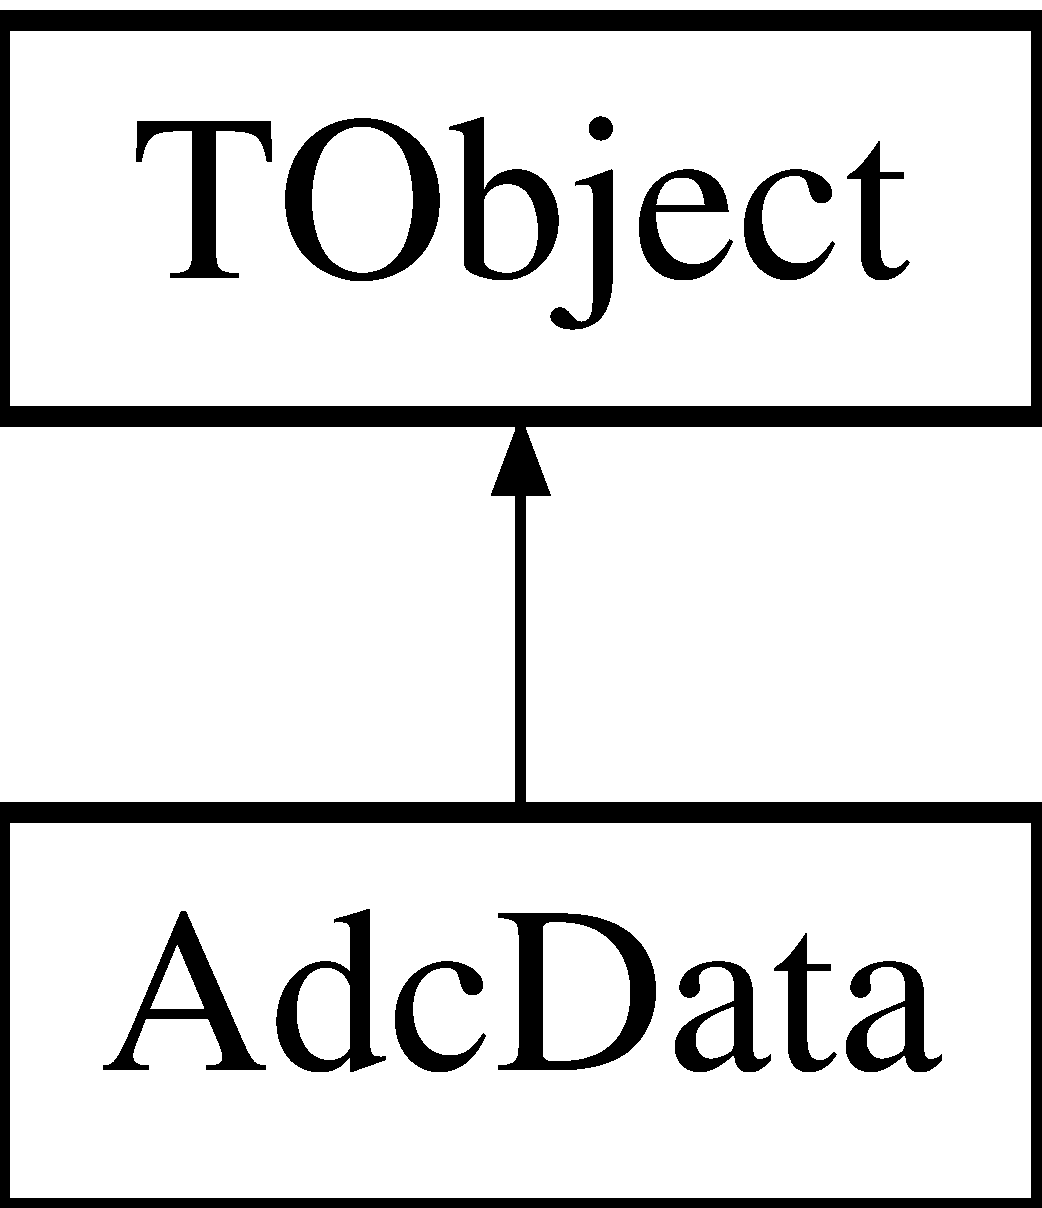
\includegraphics[height=2.000000cm]{class_adc_data}
\end{center}
\end{figure}
\subsection*{Public Member Functions}
\begin{DoxyCompactItemize}
\item 
\hypertarget{class_adc_data_a5523e3692fafaf035369a6b8c991df98}{{\bfseries Adc\-Data} (unsigned short, long long, \hyperlink{class_adc_sub_event}{Adc\-Sub\-Event} $\ast$, bool, bool, bool)}\label{class_adc_data_a5523e3692fafaf035369a6b8c991df98}

\item 
\hypertarget{class_adc_data_a2729314d57d17125c0055f7475c43c84}{long long {\bfseries Time} ()}\label{class_adc_data_a2729314d57d17125c0055f7475c43c84}

\item 
\hypertarget{class_adc_data_a026e4922b857c1015e52ecc53dc0a190}{unsigned short {\bfseries Module\-Number} ()}\label{class_adc_data_a026e4922b857c1015e52ecc53dc0a190}

\item 
\hypertarget{class_adc_data_a92ec46fe660d0e0bc3153fb736dd297d}{bool {\bfseries Laser\-On} ()}\label{class_adc_data_a92ec46fe660d0e0bc3153fb736dd297d}

\item 
\hypertarget{class_adc_data_a94785461bc83a0e6ae78d70945bf36b3}{bool {\bfseries Field\-Up} ()}\label{class_adc_data_a94785461bc83a0e6ae78d70945bf36b3}

\item 
\hypertarget{class_adc_data_a5ae609c669e0259a68c786bef783fcd7}{bool {\bfseries Field\-Down} ()}\label{class_adc_data_a5ae609c669e0259a68c786bef783fcd7}

\item 
\hypertarget{class_adc_data_a059797e6f3b3d6e65c3ee78d5b6cd3d8}{\hyperlink{class_adc_sub_event}{Adc\-Sub\-Event} $\ast$ {\bfseries Sub\-Event} ()}\label{class_adc_data_a059797e6f3b3d6e65c3ee78d5b6cd3d8}

\end{DoxyCompactItemize}
\subsection*{Protected Member Functions}
\begin{DoxyCompactItemize}
\item 
\hypertarget{class_adc_data_a812ff2254bbb02418d5926644eef19da}{{\bfseries Class\-Def} (\hyperlink{class_adc_data}{Adc\-Data}, 3)}\label{class_adc_data_a812ff2254bbb02418d5926644eef19da}

\end{DoxyCompactItemize}
\subsection*{Protected Attributes}
\begin{DoxyCompactItemize}
\item 
\hypertarget{class_adc_data_a028babb7bd1b50fa8838c92c492c6be7}{unsigned short {\bfseries f\-Module\-Number}}\label{class_adc_data_a028babb7bd1b50fa8838c92c492c6be7}

\item 
\hypertarget{class_adc_data_a81a9a850671c20d546d98c8fb6689101}{unsigned long long {\bfseries f\-Time}}\label{class_adc_data_a81a9a850671c20d546d98c8fb6689101}

\item 
\hypertarget{class_adc_data_a671528f3704f4f88de8dabc3e8c4a8de}{bool {\bfseries f\-Laser\-On}}\label{class_adc_data_a671528f3704f4f88de8dabc3e8c4a8de}

\item 
\hypertarget{class_adc_data_aa410ceb4615427d21169567727116bfa}{bool {\bfseries f\-Field\-Up}}\label{class_adc_data_aa410ceb4615427d21169567727116bfa}

\item 
\hypertarget{class_adc_data_a921b19df1c84fcd656b7ed230f733529}{bool {\bfseries f\-Field\-Down}}\label{class_adc_data_a921b19df1c84fcd656b7ed230f733529}

\item 
\hypertarget{class_adc_data_ae2c539ff0e3754c9089e3715904055ae}{\hyperlink{class_adc_sub_event}{Adc\-Sub\-Event} {\bfseries f\-Adc\-Sub\-Event}}\label{class_adc_data_ae2c539ff0e3754c9089e3715904055ae}

\end{DoxyCompactItemize}


The documentation for this class was generated from the following files\-:\begin{DoxyCompactItemize}
\item 
Med\-To\-Root/Datas.\-hh\item 
Med\-To\-Root/Datas.\-cc\end{DoxyCompactItemize}

\hypertarget{class_adc_module}{}\section{Adc\+Module Class Reference}
\label{class_adc_module}\index{Adc\+Module@{Adc\+Module}}
Inheritance diagram for Adc\+Module\+:\begin{figure}[H]
\begin{center}
\leavevmode
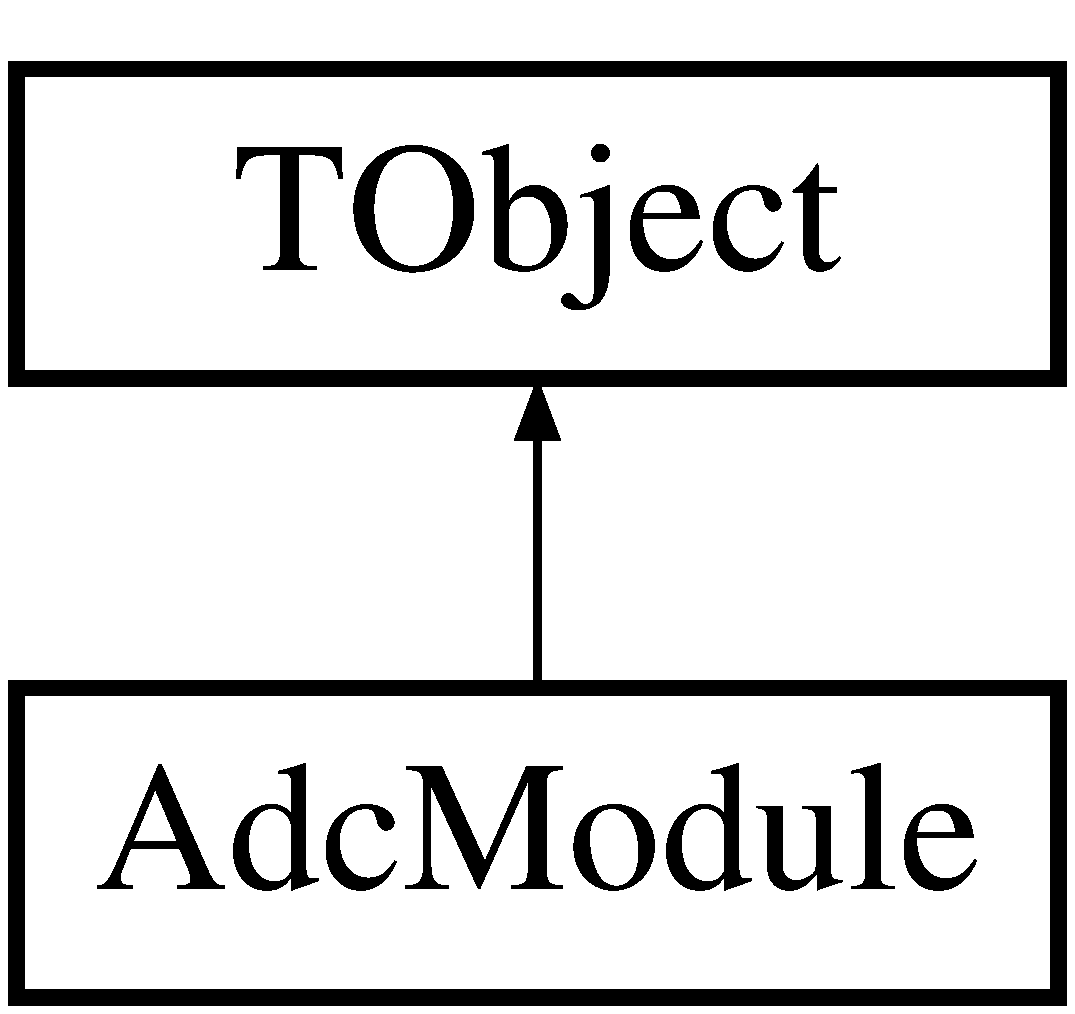
\includegraphics[height=2.000000cm]{class_adc_module}
\end{center}
\end{figure}
\subsection*{Public Member Functions}
\begin{DoxyCompactItemize}
\item 
\mbox{\Hypertarget{class_adc_module_a04ea54bf49f99a47d9b16011cf0d5efd}\label{class_adc_module_a04ea54bf49f99a47d9b16011cf0d5efd}} 
void {\bfseries Clear\+Evt} ()
\item 
\mbox{\Hypertarget{class_adc_module_a6debf2b84685eef14f16be21baa6adab}\label{class_adc_module_a6debf2b84685eef14f16be21baa6adab}} 
void {\bfseries Set\+Module\+Number} (unsigned short module\+Number)
\item 
\mbox{\Hypertarget{class_adc_module_a3a156c91cd5ba2e1195d9bc31a88bd92}\label{class_adc_module_a3a156c91cd5ba2e1195d9bc31a88bd92}} 
void {\bfseries Add\+Sub\+Event} (\hyperlink{class_adc_sub_event}{Adc\+Sub\+Event} New\+Sub\+Event)
\item 
\mbox{\Hypertarget{class_adc_module_ae8b246298ada5eb002cfefc383810ddc}\label{class_adc_module_ae8b246298ada5eb002cfefc383810ddc}} 
void {\bfseries Deleta\+Last\+Sub\+Event} ()
\item 
\mbox{\Hypertarget{class_adc_module_ae58f16947fe1a686aba589be53cfadf5}\label{class_adc_module_ae58f16947fe1a686aba589be53cfadf5}} 
size\+\_\+t {\bfseries Get\+Number\+Of\+Sub\+Events} ()
\item 
\mbox{\Hypertarget{class_adc_module_aeffd018af28812f62907bbd7e0e4bccc}\label{class_adc_module_aeffd018af28812f62907bbd7e0e4bccc}} 
unsigned short {\bfseries Get\+Module\+Number} ()
\item 
\mbox{\Hypertarget{class_adc_module_a2a5274842c08316c6cb694ecbbd502c6}\label{class_adc_module_a2a5274842c08316c6cb694ecbbd502c6}} 
\hyperlink{class_adc_sub_event}{Adc\+Sub\+Event} $\ast$ {\bfseries Get\+Sub\+Event} (size\+\_\+t Index)
\item 
\mbox{\Hypertarget{class_adc_module_a34e67e298e392a934a97c3ebad4b30e4}\label{class_adc_module_a34e67e298e392a934a97c3ebad4b30e4}} 
\hyperlink{class_adc_sub_event}{Adc\+Sub\+Event} {\bfseries Get\+Last\+Sub\+Event} ()
\end{DoxyCompactItemize}
\subsection*{Protected Attributes}
\begin{DoxyCompactItemize}
\item 
\mbox{\Hypertarget{class_adc_module_a43a09a684ccb5fc37747241697f269ee}\label{class_adc_module_a43a09a684ccb5fc37747241697f269ee}} 
unsigned short {\bfseries Module\+Number}
\item 
\mbox{\Hypertarget{class_adc_module_adb2c7c6afe959590bf3ab8df284b4518}\label{class_adc_module_adb2c7c6afe959590bf3ab8df284b4518}} 
vector$<$ \hyperlink{class_adc_sub_event}{Adc\+Sub\+Event} $>$ {\bfseries Sub\+Events}
\end{DoxyCompactItemize}


The documentation for this class was generated from the following files\+:\begin{DoxyCompactItemize}
\item 
Med\+To\+Root/Modules.\+hh\item 
Med\+To\+Root/Modules.\+cc\end{DoxyCompactItemize}

\hypertarget{class_adc_sub_event}{}\section{Adc\+Sub\+Event Class Reference}
\label{class_adc_sub_event}\index{Adc\+Sub\+Event@{Adc\+Sub\+Event}}
Inheritance diagram for Adc\+Sub\+Event\+:\begin{figure}[H]
\begin{center}
\leavevmode
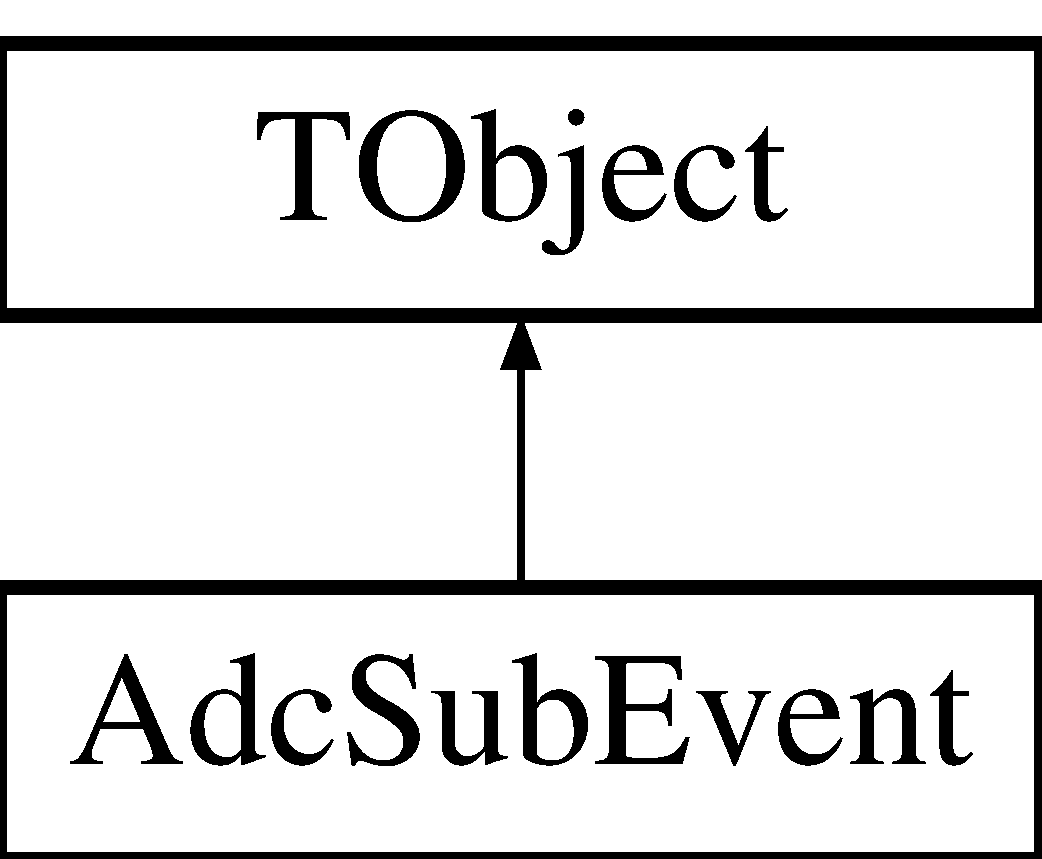
\includegraphics[height=2.000000cm]{class_adc_sub_event}
\end{center}
\end{figure}
\subsection*{Public Member Functions}
\begin{DoxyCompactItemize}
\item 
\mbox{\Hypertarget{class_adc_sub_event_a6921cc7a76de6c57de1f4505aa3a0fc6}\label{class_adc_sub_event_a6921cc7a76de6c57de1f4505aa3a0fc6}} 
void {\bfseries Clear\+Evt} ()
\item 
\mbox{\Hypertarget{class_adc_sub_event_aefa9fcc6a598d13e775ef6ab3a4c8d57}\label{class_adc_sub_event_aefa9fcc6a598d13e775ef6ab3a4c8d57}} 
size\+\_\+t {\bfseries Size} ()
\item 
\mbox{\Hypertarget{class_adc_sub_event_afff9f0777f4eed5da2e596d65247d1ff}\label{class_adc_sub_event_afff9f0777f4eed5da2e596d65247d1ff}} 
void {\bfseries Add} (unsigned short adc\+Channel, unsigned short adc\+Value)
\item 
\mbox{\Hypertarget{class_adc_sub_event_a9ae27303e054dc233160f03360f5d9db}\label{class_adc_sub_event_a9ae27303e054dc233160f03360f5d9db}} 
void {\bfseries Timestamp} (long long time\+Stamp)
\item 
\mbox{\Hypertarget{class_adc_sub_event_ae9b2f13ea3c9f93a5ad9c976aacd986e}\label{class_adc_sub_event_ae9b2f13ea3c9f93a5ad9c976aacd986e}} 
vector$<$ unsigned short $>$ {\bfseries Adc\+Channel} ()
\item 
\mbox{\Hypertarget{class_adc_sub_event_ac35e71c13f62eff54dff047c81dc87e1}\label{class_adc_sub_event_ac35e71c13f62eff54dff047c81dc87e1}} 
vector$<$ unsigned short $>$ {\bfseries Adc\+Value} ()
\item 
\mbox{\Hypertarget{class_adc_sub_event_acbd64195813827ddec628afa090978cf}\label{class_adc_sub_event_acbd64195813827ddec628afa090978cf}} 
unsigned short {\bfseries Adc\+Channel} (unsigned short Index)
\item 
\mbox{\Hypertarget{class_adc_sub_event_a076eeb66b1edcde4fa6bce1a3c5c2bb1}\label{class_adc_sub_event_a076eeb66b1edcde4fa6bce1a3c5c2bb1}} 
unsigned short {\bfseries Adc\+Value} (unsigned short Index)
\item 
\mbox{\Hypertarget{class_adc_sub_event_a3afbce187c753a266f05f56e0d46897d}\label{class_adc_sub_event_a3afbce187c753a266f05f56e0d46897d}} 
unsigned short {\bfseries Get\+Last\+Adc\+Channel} ()
\item 
\mbox{\Hypertarget{class_adc_sub_event_a14dcc9cc0d97fef0b80303ac7776019c}\label{class_adc_sub_event_a14dcc9cc0d97fef0b80303ac7776019c}} 
unsigned short {\bfseries Get\+Last\+Adc\+Value} ()
\item 
\mbox{\Hypertarget{class_adc_sub_event_ac49b638c7d81d251300a7d65a9c33e11}\label{class_adc_sub_event_ac49b638c7d81d251300a7d65a9c33e11}} 
void {\bfseries Get} (unsigned short Index, unsigned short \&adc\+Channel, unsigned short \&adc\+Value)
\item 
\mbox{\Hypertarget{class_adc_sub_event_ab76f954140f4aea1baac5bc2a109f558}\label{class_adc_sub_event_ab76f954140f4aea1baac5bc2a109f558}} 
long long {\bfseries Timestamp} ()
\end{DoxyCompactItemize}
\subsection*{Protected Attributes}
\begin{DoxyCompactItemize}
\item 
\mbox{\Hypertarget{class_adc_sub_event_a4da7e5aa53af126234c81cbcf64cfd85}\label{class_adc_sub_event_a4da7e5aa53af126234c81cbcf64cfd85}} 
long long {\bfseries f\+Timestamp}
\item 
\mbox{\Hypertarget{class_adc_sub_event_a27eefd5215bc0d882b277d627c33436d}\label{class_adc_sub_event_a27eefd5215bc0d882b277d627c33436d}} 
vector$<$ unsigned short $>$ {\bfseries f\+Adc\+Channel}
\item 
\mbox{\Hypertarget{class_adc_sub_event_a0c779d8072a161c53e3b3ac57d41a25a}\label{class_adc_sub_event_a0c779d8072a161c53e3b3ac57d41a25a}} 
vector$<$ unsigned short $>$ {\bfseries f\+Adc\+Value}
\end{DoxyCompactItemize}


The documentation for this class was generated from the following files\+:\begin{DoxyCompactItemize}
\item 
Med\+To\+Root/Sub\+Events.\+hh\item 
Med\+To\+Root/Sub\+Events.\+cc\end{DoxyCompactItemize}

\input{class_add_back}
\hypertarget{class_bragg_chamber}{}\section{Bragg\+Chamber Class Reference}
\label{class_bragg_chamber}\index{Bragg\+Chamber@{Bragg\+Chamber}}
Inheritance diagram for Bragg\+Chamber\+:\begin{figure}[H]
\begin{center}
\leavevmode
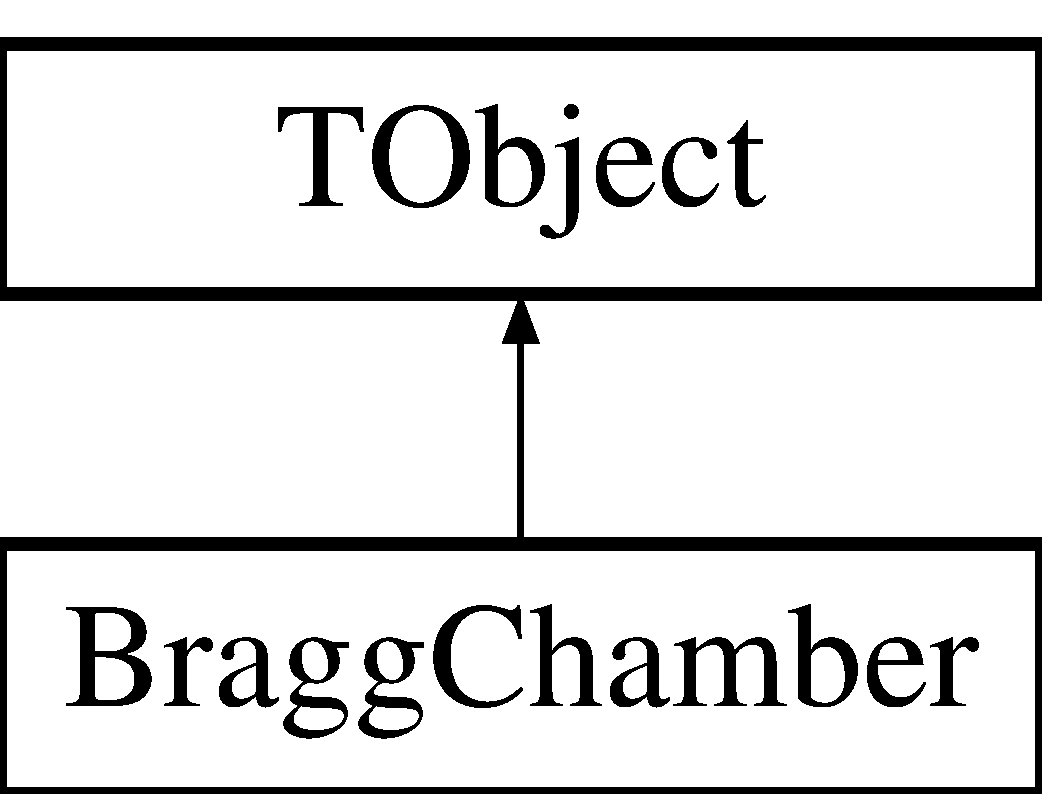
\includegraphics[height=2.000000cm]{class_bragg_chamber}
\end{center}
\end{figure}
\subsection*{Public Member Functions}
\begin{DoxyCompactItemize}
\item 
\mbox{\Hypertarget{class_bragg_chamber_ae8a4df69182d582b29182850f3aeacbe}\label{class_bragg_chamber_ae8a4df69182d582b29182850f3aeacbe}} 
void {\bfseries Clear\+Evt} ()
\item 
\mbox{\Hypertarget{class_bragg_chamber_a578cee86f2c835bcf877e89f2cc3dcc7}\label{class_bragg_chamber_a578cee86f2c835bcf877e89f2cc3dcc7}} 
void {\bfseries Add\+Sub\+Event} (\hyperlink{class_bragg_chamber_sub_event}{Bragg\+Chamber\+Sub\+Event} Sub\+Event)
\item 
\mbox{\Hypertarget{class_bragg_chamber_a5dae757b5621222d724e2aa1a36f5ac3}\label{class_bragg_chamber_a5dae757b5621222d724e2aa1a36f5ac3}} 
size\+\_\+t {\bfseries Get\+Number\+Of\+Sub\+Events} ()
\item 
\mbox{\Hypertarget{class_bragg_chamber_a03454d6f7eb1605bd0dcc5cbce199b7e}\label{class_bragg_chamber_a03454d6f7eb1605bd0dcc5cbce199b7e}} 
\hyperlink{class_bragg_chamber_sub_event}{Bragg\+Chamber\+Sub\+Event} $\ast$ {\bfseries Get\+Sub\+Event} (size\+\_\+t Index)
\item 
\mbox{\Hypertarget{class_bragg_chamber_a2bb4b74450e9d16b1634e43b86f64bf8}\label{class_bragg_chamber_a2bb4b74450e9d16b1634e43b86f64bf8}} 
\hyperlink{class_bragg_chamber_sub_event}{Bragg\+Chamber\+Sub\+Event} {\bfseries Get\+Last\+Sub\+Event} ()
\end{DoxyCompactItemize}
\subsection*{Protected Attributes}
\begin{DoxyCompactItemize}
\item 
\mbox{\Hypertarget{class_bragg_chamber_aca89325f585002ab74998709253575e3}\label{class_bragg_chamber_aca89325f585002ab74998709253575e3}} 
vector$<$ \hyperlink{class_bragg_chamber_sub_event}{Bragg\+Chamber\+Sub\+Event} $>$ {\bfseries Sub\+Events}
\end{DoxyCompactItemize}


The documentation for this class was generated from the following files\+:\begin{DoxyCompactItemize}
\item 
Med\+To\+Root/Modules.\+hh\item 
Med\+To\+Root/Modules.\+cc\end{DoxyCompactItemize}

\hypertarget{class_bragg_chamber_sub_event}{\section{Bragg\-Chamber\-Sub\-Event Class Reference}
\label{class_bragg_chamber_sub_event}\index{Bragg\-Chamber\-Sub\-Event@{Bragg\-Chamber\-Sub\-Event}}
}
Inheritance diagram for Bragg\-Chamber\-Sub\-Event\-:\begin{figure}[H]
\begin{center}
\leavevmode
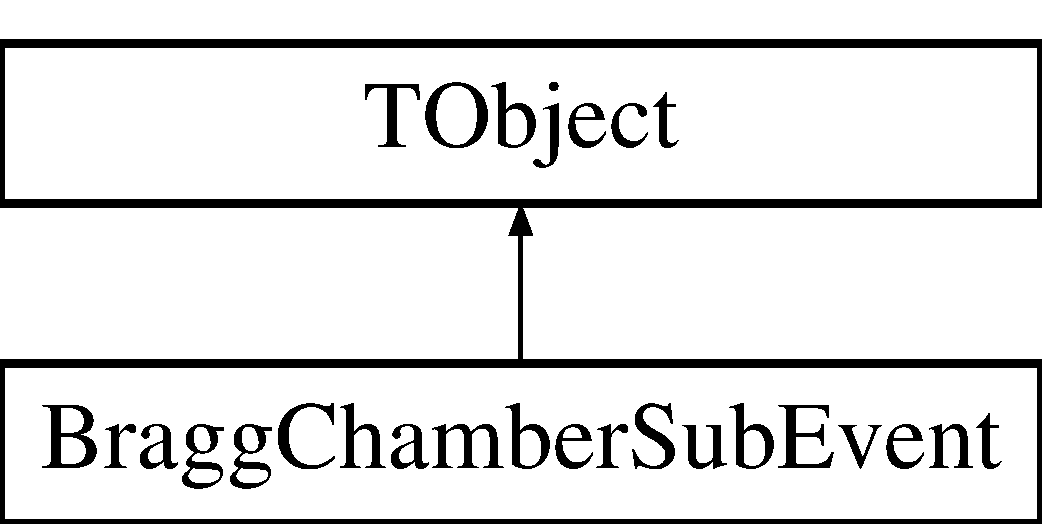
\includegraphics[height=2.000000cm]{class_bragg_chamber_sub_event}
\end{center}
\end{figure}
\subsection*{Public Member Functions}
\begin{DoxyCompactItemize}
\item 
\hypertarget{class_bragg_chamber_sub_event_a361384c90ff3a09bc91f1cc644c80e58}{void {\bfseries Clear\-Evt} ()}\label{class_bragg_chamber_sub_event_a361384c90ff3a09bc91f1cc644c80e58}

\item 
\hypertarget{class_bragg_chamber_sub_event_a04c65ccc330d71355f8b642eabf6c464}{void {\bfseries Data\-Size} (unsigned short Size)}\label{class_bragg_chamber_sub_event_a04c65ccc330d71355f8b642eabf6c464}

\item 
\hypertarget{class_bragg_chamber_sub_event_af6d6ac1acdea729f2feefad5f897ff43}{void {\bfseries Trigger} (unsigned short i, bool Trigger)}\label{class_bragg_chamber_sub_event_af6d6ac1acdea729f2feefad5f897ff43}

\item 
\hypertarget{class_bragg_chamber_sub_event_af67259ec99fc0a94706d61411567a5c9}{void {\bfseries Overflow} (unsigned short i, bool Overflow)}\label{class_bragg_chamber_sub_event_af67259ec99fc0a94706d61411567a5c9}

\item 
\hypertarget{class_bragg_chamber_sub_event_ad6b036298bc77c069005948cebd4df7e}{vector$<$ unsigned int $>$ $\ast$ {\bfseries Get\-Channel} (unsigned short i)}\label{class_bragg_chamber_sub_event_ad6b036298bc77c069005948cebd4df7e}

\item 
\hypertarget{class_bragg_chamber_sub_event_a0d98bf1a80709bcf8d36c479b9548ebd}{unsigned short {\bfseries Data\-Size} ()}\label{class_bragg_chamber_sub_event_a0d98bf1a80709bcf8d36c479b9548ebd}

\item 
\hypertarget{class_bragg_chamber_sub_event_a2723e90238f9d3545f40d305621d7ec7}{bool {\bfseries Trigger} (unsigned short i)}\label{class_bragg_chamber_sub_event_a2723e90238f9d3545f40d305621d7ec7}

\item 
\hypertarget{class_bragg_chamber_sub_event_adca2567c05cb94ed4336ac0516d5e63a}{bool {\bfseries Overflow} (unsigned short i)}\label{class_bragg_chamber_sub_event_adca2567c05cb94ed4336ac0516d5e63a}

\end{DoxyCompactItemize}
\subsection*{Protected Attributes}
\begin{DoxyCompactItemize}
\item 
\hypertarget{class_bragg_chamber_sub_event_aa5205f96a716ea517af677c074367d9a}{unsigned short {\bfseries f\-Data\-Size}}\label{class_bragg_chamber_sub_event_aa5205f96a716ea517af677c074367d9a}

\item 
\hypertarget{class_bragg_chamber_sub_event_ac33e87b9327b80f85032de6076f1986e}{bool {\bfseries f\-Trigger} \mbox{[}Number\-Of\-Bragg\-Channels\mbox{]}}\label{class_bragg_chamber_sub_event_ac33e87b9327b80f85032de6076f1986e}

\item 
\hypertarget{class_bragg_chamber_sub_event_a59f31e1a784e52768d19bfd98dae16f0}{bool {\bfseries f\-Overflow} \mbox{[}Number\-Of\-Bragg\-Channels\mbox{]}}\label{class_bragg_chamber_sub_event_a59f31e1a784e52768d19bfd98dae16f0}

\item 
\hypertarget{class_bragg_chamber_sub_event_a12a0e9050a32c41872751696a6c4606e}{vector$<$ unsigned int $>$ {\bfseries f\-Data} \mbox{[}Number\-Of\-Bragg\-Channels\mbox{]}}\label{class_bragg_chamber_sub_event_a12a0e9050a32c41872751696a6c4606e}

\end{DoxyCompactItemize}


The documentation for this class was generated from the following files\-:\begin{DoxyCompactItemize}
\item 
Med\-To\-Root/Sub\-Events.\-hh\item 
Med\-To\-Root/Sub\-Events.\-cc\end{DoxyCompactItemize}

\hypertarget{class_built_event}{}\section{Built\+Event Class Reference}
\label{class_built_event}\index{Built\+Event@{Built\+Event}}
Inheritance diagram for Built\+Event\+:\begin{figure}[H]
\begin{center}
\leavevmode
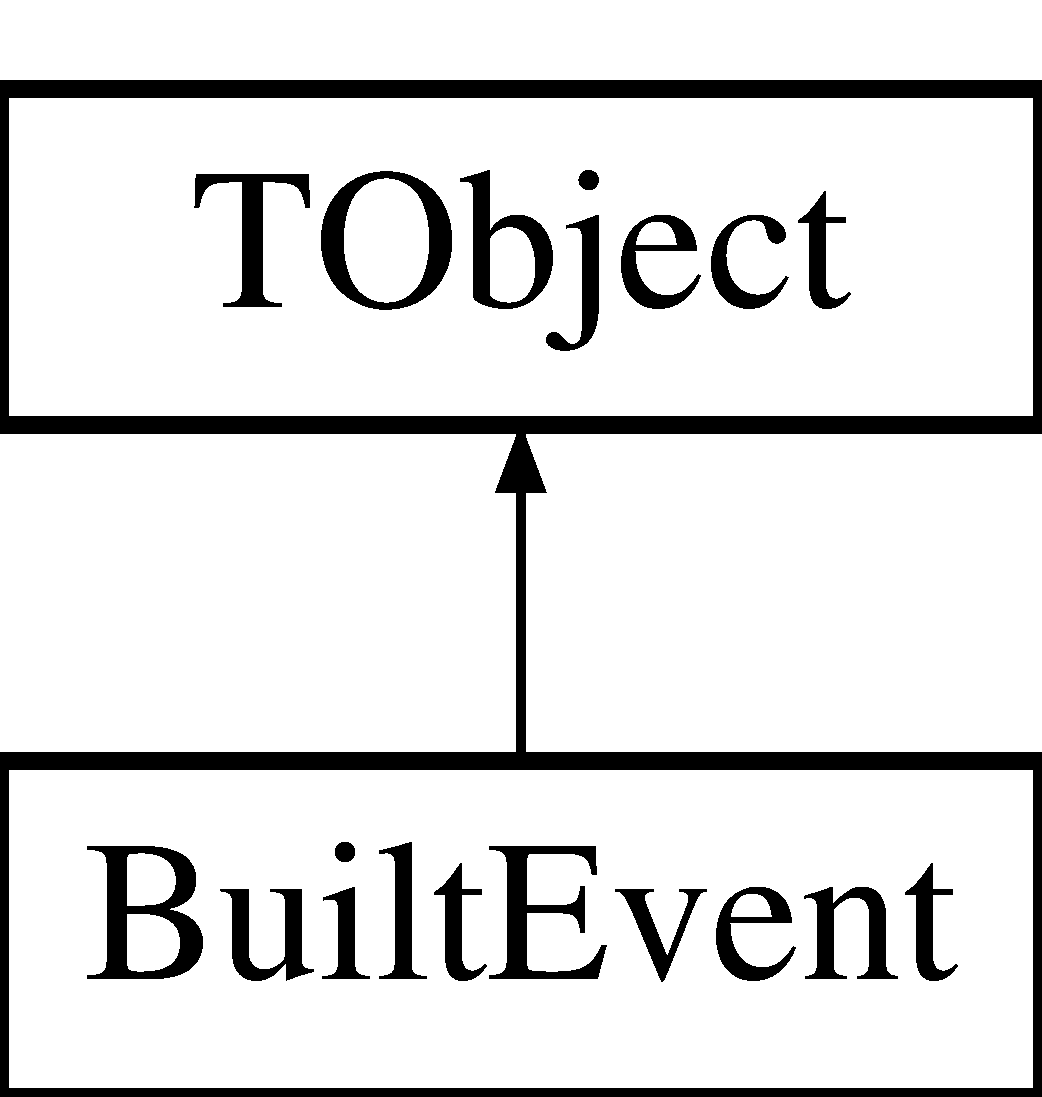
\includegraphics[height=2.000000cm]{class_built_event}
\end{center}
\end{figure}
\subsection*{Public Member Functions}
\begin{DoxyCompactItemize}
\item 
\mbox{\Hypertarget{class_built_event_a6191c8fda84fcc3ab2ce774db393db18}\label{class_built_event_a6191c8fda84fcc3ab2ce774db393db18}} 
{\bfseries Built\+Event} (unsigned short, \hyperlink{class_adc_sub_event}{Adc\+Sub\+Event} $\ast$, long long, bool, bool, bool)
\item 
\mbox{\Hypertarget{class_built_event_ae9580318d1344acfc33d4e603d31f058}\label{class_built_event_ae9580318d1344acfc33d4e603d31f058}} 
{\bfseries Built\+Event} (unsigned short, unsigned short, \hyperlink{class_dgf_sub_event}{Dgf\+Sub\+Event} $\ast$)
\item 
\mbox{\Hypertarget{class_built_event_a332515d3db4d4e0b324a4584090d78e3}\label{class_built_event_a332515d3db4d4e0b324a4584090d78e3}} 
void {\bfseries Clear\+Evt} ()
\item 
\mbox{\Hypertarget{class_built_event_a3f521359cd9e884f3eaba119ef8f6102}\label{class_built_event_a3f521359cd9e884f3eaba119ef8f6102}} 
void {\bfseries Add\+Particle} (unsigned short, \hyperlink{class_adc_sub_event}{Adc\+Sub\+Event} $\ast$, long long, bool, bool, bool)
\item 
\mbox{\Hypertarget{class_built_event_ae7e96358bcd4b95f4908ed0eff1be292}\label{class_built_event_ae7e96358bcd4b95f4908ed0eff1be292}} 
void {\bfseries Add\+Gamma} (unsigned short, unsigned short, \hyperlink{class_dgf_sub_event}{Dgf\+Sub\+Event} $\ast$, unsigned short)
\item 
\mbox{\Hypertarget{class_built_event_a4c1868b1cd5d9e2e143db1feebe51b40}\label{class_built_event_a4c1868b1cd5d9e2e143db1feebe51b40}} 
void {\bfseries Add\+Timing} (long long Ebis\+Time, long long T1\+Time, long long Super\+Cycle\+Time)
\item 
\mbox{\Hypertarget{class_built_event_ad3dfcf9a541516c8c9bc391ca91e8748}\label{class_built_event_ad3dfcf9a541516c8c9bc391ca91e8748}} 
void {\bfseries Event\+Number} (long long Event\+Number)
\item 
\mbox{\Hypertarget{class_built_event_a71a6879f3cb5a2d2714c17152c569c41}\label{class_built_event_a71a6879f3cb5a2d2714c17152c569c41}} 
void {\bfseries Sub\+Event\+Number} (unsigned short Sub\+Event\+Number)
\item 
\mbox{\Hypertarget{class_built_event_a1e50f0e800d504e04dbf62ddd9ba9b0d}\label{class_built_event_a1e50f0e800d504e04dbf62ddd9ba9b0d}} 
size\+\_\+t {\bfseries Number\+Of\+Adcs} ()
\item 
\mbox{\Hypertarget{class_built_event_a5c01e6c2ada2435c6d7309dc7cb2fa5c}\label{class_built_event_a5c01e6c2ada2435c6d7309dc7cb2fa5c}} 
size\+\_\+t {\bfseries Number\+Of\+Dgfs} ()
\item 
\mbox{\Hypertarget{class_built_event_aac0e9789b3e193a60c28a8c7643c37c1}\label{class_built_event_aac0e9789b3e193a60c28a8c7643c37c1}} 
long long {\bfseries Ebis\+Time} ()
\item 
\mbox{\Hypertarget{class_built_event_adbe7cecefb72c1429bb46fb38839b6ed}\label{class_built_event_adbe7cecefb72c1429bb46fb38839b6ed}} 
long long {\bfseries T1\+Time} ()
\item 
\mbox{\Hypertarget{class_built_event_a3bcfcdef39836deeae613b1feadce8ca}\label{class_built_event_a3bcfcdef39836deeae613b1feadce8ca}} 
long long {\bfseries Super\+Cycle\+Time} ()
\item 
\mbox{\Hypertarget{class_built_event_a699e90b7621ae7e8e139c0f9f7ac36df}\label{class_built_event_a699e90b7621ae7e8e139c0f9f7ac36df}} 
long long {\bfseries Event\+Number} ()
\item 
\mbox{\Hypertarget{class_built_event_a634ff74c48a2414782e5b55a606d9c02}\label{class_built_event_a634ff74c48a2414782e5b55a606d9c02}} 
unsigned short {\bfseries Sub\+Event\+Number} ()
\item 
\mbox{\Hypertarget{class_built_event_aa031a6f9f75054f4bcd34a5ae0434211}\label{class_built_event_aa031a6f9f75054f4bcd34a5ae0434211}} 
\hyperlink{class_adc_data}{Adc\+Data} $\ast$ {\bfseries Adc} (size\+\_\+t Index)
\item 
\mbox{\Hypertarget{class_built_event_ad0baf9c54126df4ef5be7110283d1a4d}\label{class_built_event_ad0baf9c54126df4ef5be7110283d1a4d}} 
\hyperlink{class_dgf_data}{Dgf\+Data} $\ast$ {\bfseries Dgf} (size\+\_\+t Index)
\item 
\mbox{\Hypertarget{class_built_event_a264f67ad32d955fa2ff389c923bc69b0}\label{class_built_event_a264f67ad32d955fa2ff389c923bc69b0}} 
bool {\bfseries Coincident} (\hyperlink{class_global_settings}{Global\+Settings} $\ast$, long long)
\item 
\mbox{\Hypertarget{class_built_event_af5244b5b93aa8e0adfcaf3fa70be5617}\label{class_built_event_af5244b5b93aa8e0adfcaf3fa70be5617}} 
long long {\bfseries Get\+Time} ()
\end{DoxyCompactItemize}
\subsection*{Protected Attributes}
\begin{DoxyCompactItemize}
\item 
\mbox{\Hypertarget{class_built_event_a03d3a46cd8ffa584750f814895a36719}\label{class_built_event_a03d3a46cd8ffa584750f814895a36719}} 
long long {\bfseries ebis\+Time}
\item 
\mbox{\Hypertarget{class_built_event_a7a57667e365324e20b3cd27411bf27a4}\label{class_built_event_a7a57667e365324e20b3cd27411bf27a4}} 
long long {\bfseries t1\+Time}
\item 
\mbox{\Hypertarget{class_built_event_af4382a0a57b77db32d3934fa2764109f}\label{class_built_event_af4382a0a57b77db32d3934fa2764109f}} 
long long {\bfseries super\+Cycle\+Time}
\item 
\mbox{\Hypertarget{class_built_event_a2492458c6571f5bbbb4d4083b380bf33}\label{class_built_event_a2492458c6571f5bbbb4d4083b380bf33}} 
long long {\bfseries event\+Number}
\item 
\mbox{\Hypertarget{class_built_event_ab0b418e8733a07abbe5008d0b0dd4263}\label{class_built_event_ab0b418e8733a07abbe5008d0b0dd4263}} 
unsigned int {\bfseries sub\+Event\+Number}
\item 
\mbox{\Hypertarget{class_built_event_adeb272a29e4b64150197eb14d8f99d9c}\label{class_built_event_adeb272a29e4b64150197eb14d8f99d9c}} 
vector$<$ \hyperlink{class_adc_data}{Adc\+Data} $>$ {\bfseries adc\+Data}
\item 
\mbox{\Hypertarget{class_built_event_acec847a035bef94b9820e31d1d1468ee}\label{class_built_event_acec847a035bef94b9820e31d1d1468ee}} 
vector$<$ \hyperlink{class_dgf_data}{Dgf\+Data} $>$ {\bfseries dgf\+Data}
\end{DoxyCompactItemize}


The documentation for this class was generated from the following files\+:\begin{DoxyCompactItemize}
\item 
Med\+To\+Root/Built\+Event.\+hh\item 
Med\+To\+Root/Built\+Event.\+cc\end{DoxyCompactItemize}

\hypertarget{class_calibration}{}\section{Calibration Class Reference}
\label{class_calibration}\index{Calibration@{Calibration}}


{\ttfamily \#include $<$Calibration.\+hh$>$}

\subsection*{Public Member Functions}
\begin{DoxyCompactItemize}
\item 
\mbox{\Hypertarget{class_calibration_a981f7a519754aecbdd3fbd837a5b5762}\label{class_calibration_a981f7a519754aecbdd3fbd837a5b5762}} 
{\bfseries Calibration} (const char $\ast$)
\item 
\mbox{\Hypertarget{class_calibration_ad675a1c74ecd23e3af37fcffdeeed246}\label{class_calibration_ad675a1c74ecd23e3af37fcffdeeed246}} 
void {\bfseries Read\+Calibration} ()
\item 
\mbox{\Hypertarget{class_calibration_af224d188d64080db8d14eb0ddbb909f7}\label{class_calibration_af224d188d64080db8d14eb0ddbb909f7}} 
void {\bfseries Print\+Calibration} ()
\item 
\mbox{\Hypertarget{class_calibration_aec8340a8b2134c9cb51b685c928c4cee}\label{class_calibration_aec8340a8b2134c9cb51b685c928c4cee}} 
void {\bfseries Set\+File} (const char $\ast$filename)
\item 
\mbox{\Hypertarget{class_calibration_a10affa676c2fb505d3075d23c3bf0157}\label{class_calibration_a10affa676c2fb505d3075d23c3bf0157}} 
const string {\bfseries Input\+File} ()
\item 
\mbox{\Hypertarget{class_calibration_a0ea90a9b417ec5e50312b4bba2875f70}\label{class_calibration_a0ea90a9b417ec5e50312b4bba2875f70}} 
double {\bfseries Dgf\+Energy} (int dgf, int chan, unsigned short raw)
\item 
\mbox{\Hypertarget{class_calibration_a07ba44fdc31250e347939588759d2796}\label{class_calibration_a07ba44fdc31250e347939588759d2796}} 
double {\bfseries Adc\+Energy} (int adc, int chan, unsigned short raw)
\item 
\mbox{\Hypertarget{class_calibration_a860b3c2c4a2350009bbbf337aa56a212}\label{class_calibration_a860b3c2c4a2350009bbbf337aa56a212}} 
double {\bfseries Adc\+Time} (int adc)
\item 
\mbox{\Hypertarget{class_calibration_a65ab7c201643a2bc8cb366b9ac20ab3b}\label{class_calibration_a65ab7c201643a2bc8cb366b9ac20ab3b}} 
int {\bfseries Pos\+F\+B\+C\+D\+Ring} (int Quad, unsigned short raw)
\item 
\mbox{\Hypertarget{class_calibration_a9ee9ef612f7485f5371916bf524bb036}\label{class_calibration_a9ee9ef612f7485f5371916bf524bb036}} 
int {\bfseries Pos\+F\+B\+C\+D\+Strip} (int Quad, unsigned short raw)
\item 
\mbox{\Hypertarget{class_calibration_a240b3ac33e55af3f762d2cecc5d06b2b}\label{class_calibration_a240b3ac33e55af3f762d2cecc5d06b2b}} 
int {\bfseries Pos\+Ring} (int Quad, unsigned short raw)
\item 
\mbox{\Hypertarget{class_calibration_a1d12aea9e2be55852b937e8be3ffbae1}\label{class_calibration_a1d12aea9e2be55852b937e8be3ffbae1}} 
int {\bfseries Pos\+Strip} (int Quad, unsigned short raw)
\item 
\mbox{\Hypertarget{class_calibration_af2ce93c038cdfd3e9fb1e4ffa093097c}\label{class_calibration_af2ce93c038cdfd3e9fb1e4ffa093097c}} 
int {\bfseries Strip\+Pos\+Barrel} (unsigned short strraw, unsigned short rearraw)
\end{DoxyCompactItemize}


\subsection{Detailed Description}
A class to read in the calibration file in R\+O\+OT\textquotesingle{}s T\+Config format. Each A\+DC and D\+GF channel can have offset, gain and quadratic terms. There is potential to include the demux of T/\+C-\/\+R\+EX in here too. 

The documentation for this class was generated from the following files\+:\begin{DoxyCompactItemize}
\item 
Tree\+Builder/Calibration.\+hh\item 
Tree\+Builder/Calibration.\+cc\end{DoxyCompactItemize}

\hypertarget{class_dgf_data}{\section{Dgf\-Data Class Reference}
\label{class_dgf_data}\index{Dgf\-Data@{Dgf\-Data}}
}
Inheritance diagram for Dgf\-Data\-:\begin{figure}[H]
\begin{center}
\leavevmode
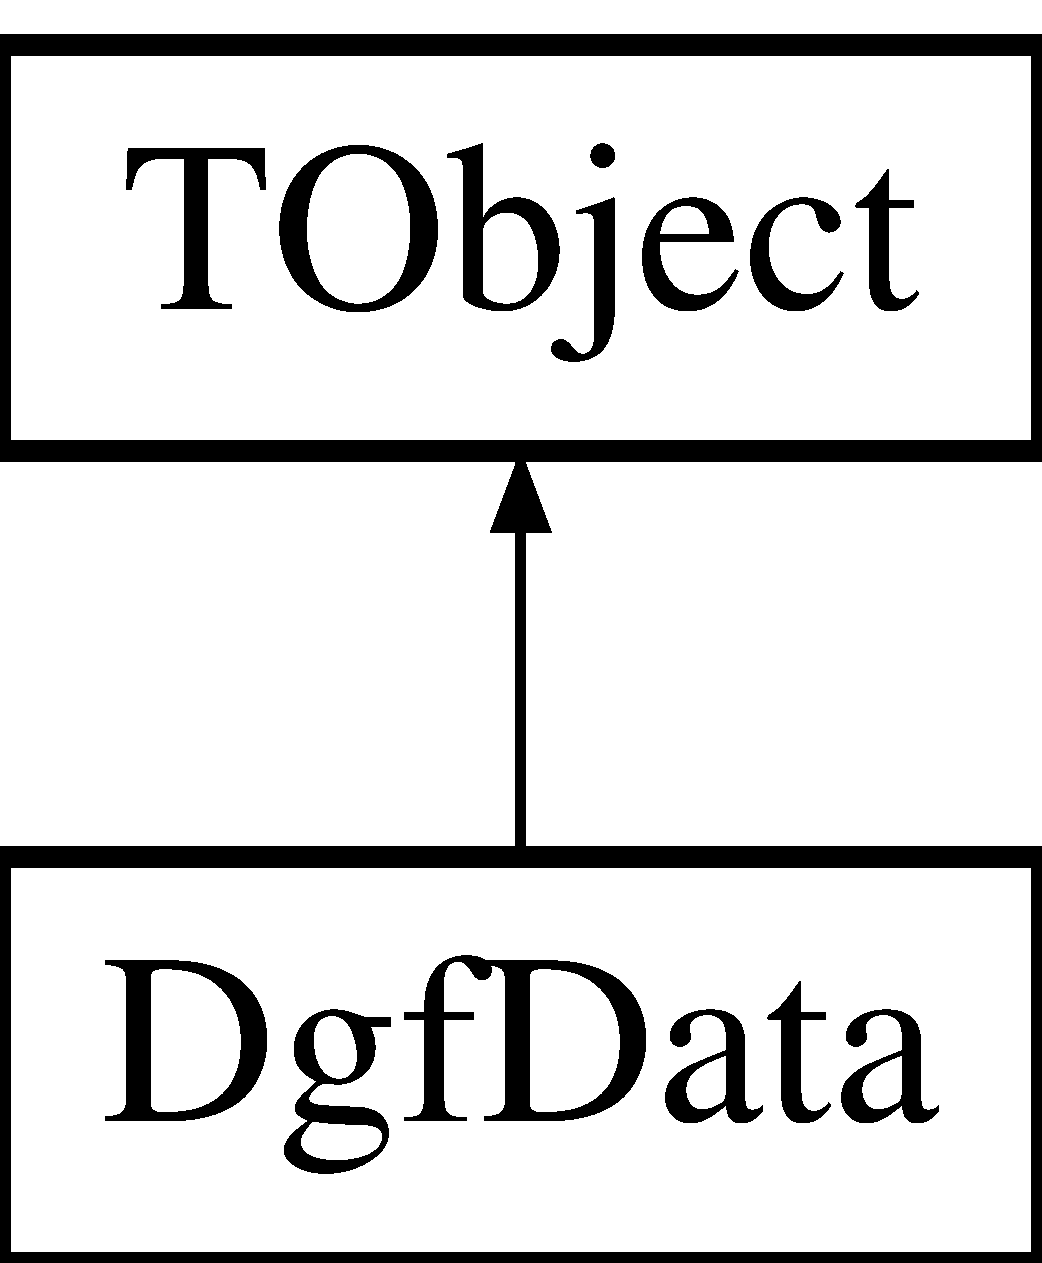
\includegraphics[height=2.000000cm]{class_dgf_data}
\end{center}
\end{figure}
\subsection*{Public Member Functions}
\begin{DoxyCompactItemize}
\item 
\hypertarget{class_dgf_data_a920d0f59bab2274d5e4ef3e80ea1a79e}{{\bfseries Dgf\-Data} (unsigned short, unsigned short, \hyperlink{class_dgf_sub_event}{Dgf\-Sub\-Event} $\ast$, unsigned short=1)}\label{class_dgf_data_a920d0f59bab2274d5e4ef3e80ea1a79e}

\item 
\hypertarget{class_dgf_data_a55d760ffcd84c99875532506563393eb}{unsigned short {\bfseries Module\-Number} ()}\label{class_dgf_data_a55d760ffcd84c99875532506563393eb}

\item 
\hypertarget{class_dgf_data_a37c740809015bde32af4220d15616b89}{unsigned short {\bfseries Channel} ()}\label{class_dgf_data_a37c740809015bde32af4220d15616b89}

\item 
\hypertarget{class_dgf_data_adbf9d6108fb3a0a79d119d941a3604ac}{unsigned short {\bfseries Multiplicity} ()}\label{class_dgf_data_adbf9d6108fb3a0a79d119d941a3604ac}

\item 
\hypertarget{class_dgf_data_a7cb7c0ac2a7553f9cb5512e781eb8d75}{unsigned short {\bfseries Energy} ()}\label{class_dgf_data_a7cb7c0ac2a7553f9cb5512e781eb8d75}

\item 
\hypertarget{class_dgf_data_a63542c903350303507d6f07f900660f6}{unsigned short $\ast$ {\bfseries User\-Values} ()}\label{class_dgf_data_a63542c903350303507d6f07f900660f6}

\item 
\hypertarget{class_dgf_data_a836a43c2de36765b3a6acd16907b47e2}{long long {\bfseries Time} ()}\label{class_dgf_data_a836a43c2de36765b3a6acd16907b47e2}

\end{DoxyCompactItemize}
\subsection*{Protected Member Functions}
\begin{DoxyCompactItemize}
\item 
\hypertarget{class_dgf_data_a2347fc4e4a77bba56c25f979f2a9fc14}{{\bfseries Class\-Def} (\hyperlink{class_dgf_data}{Dgf\-Data}, 2)}\label{class_dgf_data_a2347fc4e4a77bba56c25f979f2a9fc14}

\end{DoxyCompactItemize}
\subsection*{Protected Attributes}
\begin{DoxyCompactItemize}
\item 
\hypertarget{class_dgf_data_a4d69c87a370a0451ddad97148e6f1ad5}{unsigned short {\bfseries f\-Module\-Number}}\label{class_dgf_data_a4d69c87a370a0451ddad97148e6f1ad5}

\item 
\hypertarget{class_dgf_data_ab3184c2ceca7dcfe3d8374f42c6bd398}{unsigned short {\bfseries f\-Channel}}\label{class_dgf_data_ab3184c2ceca7dcfe3d8374f42c6bd398}

\item 
\hypertarget{class_dgf_data_a34644ed74a2c8884d51b38fc49247925}{unsigned short {\bfseries f\-Multiplicity}}\label{class_dgf_data_a34644ed74a2c8884d51b38fc49247925}

\item 
\hypertarget{class_dgf_data_a8f7d1c87b06dbe1018b267b5410470d7}{unsigned long long {\bfseries f\-Event\-Time}}\label{class_dgf_data_a8f7d1c87b06dbe1018b267b5410470d7}

\item 
\hypertarget{class_dgf_data_abab9885fd2b0bae4459f5c98d6886784}{unsigned short {\bfseries f\-Energy}}\label{class_dgf_data_abab9885fd2b0bae4459f5c98d6886784}

\item 
\hypertarget{class_dgf_data_a9dbabd6693e7b930ee8d3900030a5a86}{unsigned short {\bfseries f\-Fast\-Trigger\-Time}}\label{class_dgf_data_a9dbabd6693e7b930ee8d3900030a5a86}

\item 
\hypertarget{class_dgf_data_a1132a37b4a42fde6155f641a97ac2353}{unsigned long long {\bfseries f\-Long\-Fast\-Trigger\-Time}}\label{class_dgf_data_a1132a37b4a42fde6155f641a97ac2353}

\item 
\hypertarget{class_dgf_data_a91de5e4d052cf02e461bf1d8021dc78e}{unsigned short {\bfseries f\-User\-Values} \mbox{[}Number\-Of\-User\-Values\mbox{]}}\label{class_dgf_data_a91de5e4d052cf02e461bf1d8021dc78e}

\end{DoxyCompactItemize}


The documentation for this class was generated from the following files\-:\begin{DoxyCompactItemize}
\item 
Med\-To\-Root/Datas.\-hh\item 
Med\-To\-Root/Datas.\-cc\end{DoxyCompactItemize}

\hypertarget{class_dgf_module}{}\section{Dgf\+Module Class Reference}
\label{class_dgf_module}\index{Dgf\+Module@{Dgf\+Module}}
Inheritance diagram for Dgf\+Module\+:\begin{figure}[H]
\begin{center}
\leavevmode
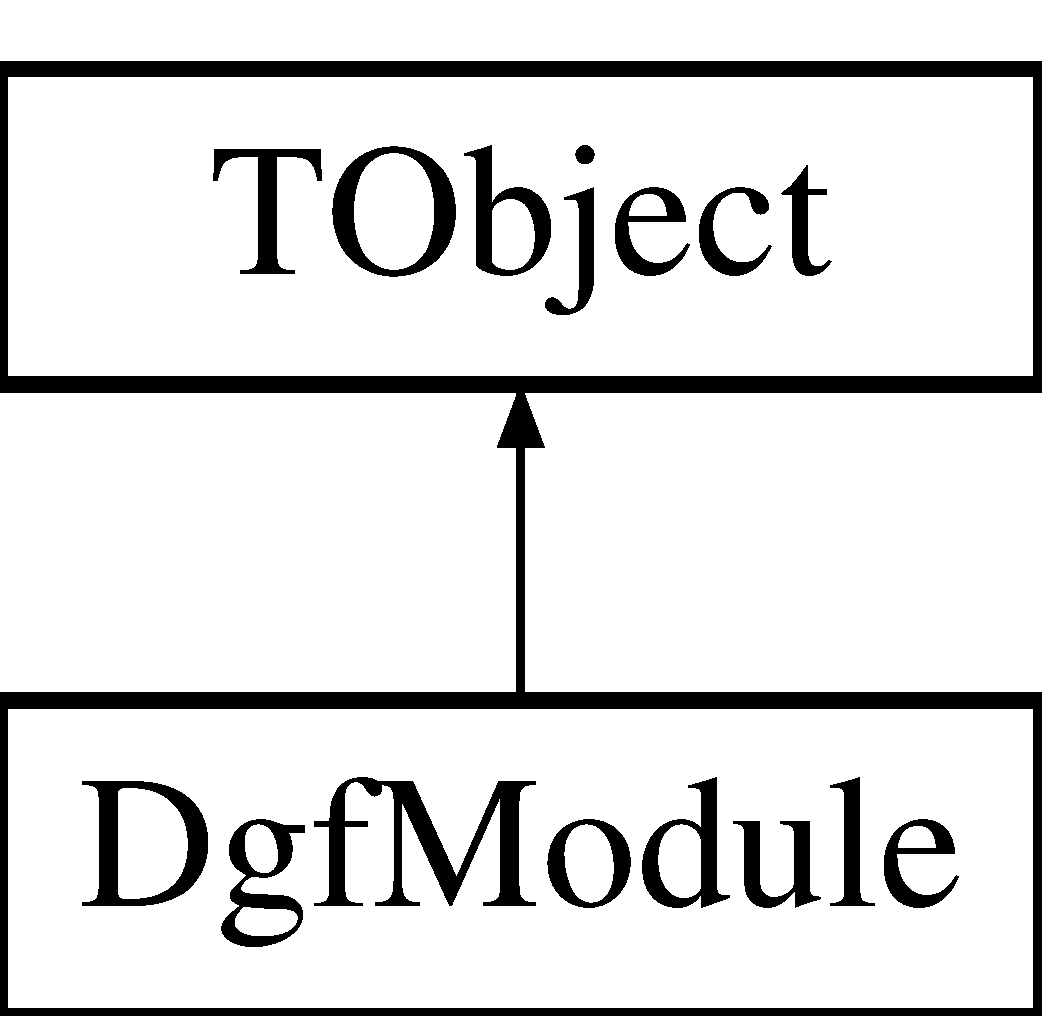
\includegraphics[height=2.000000cm]{class_dgf_module}
\end{center}
\end{figure}
\subsection*{Public Member Functions}
\begin{DoxyCompactItemize}
\item 
\mbox{\Hypertarget{class_dgf_module_a57667b7eedf5f736b575d32b29ec4ba3}\label{class_dgf_module_a57667b7eedf5f736b575d32b29ec4ba3}} 
void {\bfseries Add\+Sub\+Event} (\hyperlink{class_dgf_sub_event}{Dgf\+Sub\+Event} New\+Sub\+Event)
\item 
\mbox{\Hypertarget{class_dgf_module_a2723a18e784f5292ec9ba1f417e699a3}\label{class_dgf_module_a2723a18e784f5292ec9ba1f417e699a3}} 
void {\bfseries Clear\+Evt} ()
\item 
\mbox{\Hypertarget{class_dgf_module_a44c6164a64dc7543c57fd1f399477b46}\label{class_dgf_module_a44c6164a64dc7543c57fd1f399477b46}} 
void {\bfseries Set\+Module\+Number} (unsigned short module\+Number)
\item 
\mbox{\Hypertarget{class_dgf_module_ad9577d76d5ca21546fdebce9f6183f9d}\label{class_dgf_module_ad9577d76d5ca21546fdebce9f6183f9d}} 
void {\bfseries Set\+Type} (unsigned short type)
\item 
\mbox{\Hypertarget{class_dgf_module_afa5b0d56e89f4427fb4facb338897d92}\label{class_dgf_module_afa5b0d56e89f4427fb4facb338897d92}} 
unsigned short {\bfseries Get\+Module\+Number} ()
\item 
\mbox{\Hypertarget{class_dgf_module_a338db9255ddcd3fcb58c9678561e9210}\label{class_dgf_module_a338db9255ddcd3fcb58c9678561e9210}} 
unsigned short {\bfseries Get\+Type} ()
\item 
\mbox{\Hypertarget{class_dgf_module_aecd2134604c63c0b962318f6e8f928c1}\label{class_dgf_module_aecd2134604c63c0b962318f6e8f928c1}} 
size\+\_\+t {\bfseries Get\+Number\+Of\+Sub\+Events} ()
\item 
\mbox{\Hypertarget{class_dgf_module_a398e1293245266eee289f004b3f14ca0}\label{class_dgf_module_a398e1293245266eee289f004b3f14ca0}} 
\hyperlink{class_dgf_sub_event}{Dgf\+Sub\+Event} $\ast$ {\bfseries Get\+Sub\+Event} (size\+\_\+t Index)
\end{DoxyCompactItemize}
\subsection*{Protected Attributes}
\begin{DoxyCompactItemize}
\item 
\mbox{\Hypertarget{class_dgf_module_a06f12e7fd7e2353c454d91884fcf2bbd}\label{class_dgf_module_a06f12e7fd7e2353c454d91884fcf2bbd}} 
unsigned short {\bfseries f\+Module\+Number}
\item 
\mbox{\Hypertarget{class_dgf_module_a126da76a1c1329ce3f896371d0ba7ca1}\label{class_dgf_module_a126da76a1c1329ce3f896371d0ba7ca1}} 
unsigned short {\bfseries f\+Type}
\item 
\mbox{\Hypertarget{class_dgf_module_a0f969bc0853fa696d9ecf93ad1156f27}\label{class_dgf_module_a0f969bc0853fa696d9ecf93ad1156f27}} 
vector$<$ \hyperlink{class_dgf_sub_event}{Dgf\+Sub\+Event} $>$ {\bfseries f\+Sub\+Events}
\end{DoxyCompactItemize}


The documentation for this class was generated from the following files\+:\begin{DoxyCompactItemize}
\item 
Med\+To\+Root/Modules.\+hh\item 
Med\+To\+Root/Modules.\+cc\end{DoxyCompactItemize}

\hypertarget{class_dgf_scaler}{}\section{Dgf\+Scaler Class Reference}
\label{class_dgf_scaler}\index{Dgf\+Scaler@{Dgf\+Scaler}}
Inheritance diagram for Dgf\+Scaler\+:\begin{figure}[H]
\begin{center}
\leavevmode
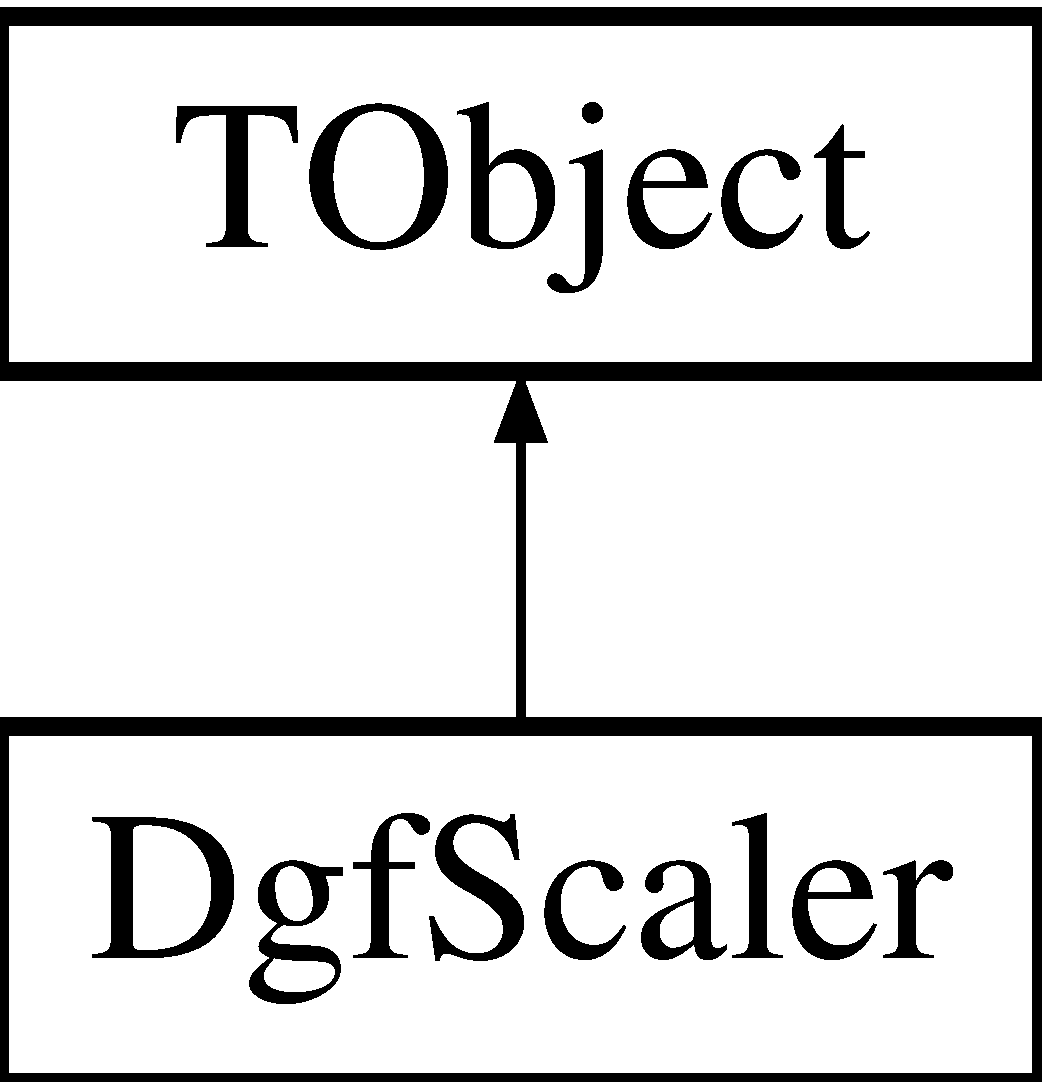
\includegraphics[height=2.000000cm]{class_dgf_scaler}
\end{center}
\end{figure}
\subsection*{Public Member Functions}
\begin{DoxyCompactItemize}
\item 
\mbox{\Hypertarget{class_dgf_scaler_a379aef078983f0664a92af66b0ef595d}\label{class_dgf_scaler_a379aef078983f0664a92af66b0ef595d}} 
void {\bfseries Clear\+Evt} ()
\item 
\mbox{\Hypertarget{class_dgf_scaler_a620d4a4dc60fd0a2608bfeb32329780e}\label{class_dgf_scaler_a620d4a4dc60fd0a2608bfeb32329780e}} 
void {\bfseries Add\+Sub\+Event} (\hyperlink{class_dgf_scaler_sub_event}{Dgf\+Scaler\+Sub\+Event} \&Sub\+Event)
\item 
\mbox{\Hypertarget{class_dgf_scaler_a1ffa8daad855bc1abda26fa647add076}\label{class_dgf_scaler_a1ffa8daad855bc1abda26fa647add076}} 
size\+\_\+t {\bfseries Get\+Number\+Of\+Sub\+Events} ()
\item 
\mbox{\Hypertarget{class_dgf_scaler_a115de3afca80d77ba524de5da88f6214}\label{class_dgf_scaler_a115de3afca80d77ba524de5da88f6214}} 
\hyperlink{class_dgf_scaler_sub_event}{Dgf\+Scaler\+Sub\+Event} $\ast$ {\bfseries Get\+Sub\+Event} (size\+\_\+t Index)
\item 
\mbox{\Hypertarget{class_dgf_scaler_a055a0de3e930c7ff88eede1adb74a52e}\label{class_dgf_scaler_a055a0de3e930c7ff88eede1adb74a52e}} 
\hyperlink{class_dgf_scaler_sub_event}{Dgf\+Scaler\+Sub\+Event} {\bfseries Get\+Last\+Sub\+Event} ()
\end{DoxyCompactItemize}
\subsection*{Protected Attributes}
\begin{DoxyCompactItemize}
\item 
\mbox{\Hypertarget{class_dgf_scaler_a867e6953afa484ee4b7ca8ec204a1fa1}\label{class_dgf_scaler_a867e6953afa484ee4b7ca8ec204a1fa1}} 
vector$<$ \hyperlink{class_dgf_scaler_sub_event}{Dgf\+Scaler\+Sub\+Event} $>$ {\bfseries Sub\+Events}
\end{DoxyCompactItemize}


The documentation for this class was generated from the following files\+:\begin{DoxyCompactItemize}
\item 
Med\+To\+Root/Modules.\+hh\item 
Med\+To\+Root/Modules.\+cc\end{DoxyCompactItemize}

\hypertarget{class_dgf_scaler_sub_event}{}\section{Dgf\+Scaler\+Sub\+Event Class Reference}
\label{class_dgf_scaler_sub_event}\index{Dgf\+Scaler\+Sub\+Event@{Dgf\+Scaler\+Sub\+Event}}
Inheritance diagram for Dgf\+Scaler\+Sub\+Event\+:\begin{figure}[H]
\begin{center}
\leavevmode
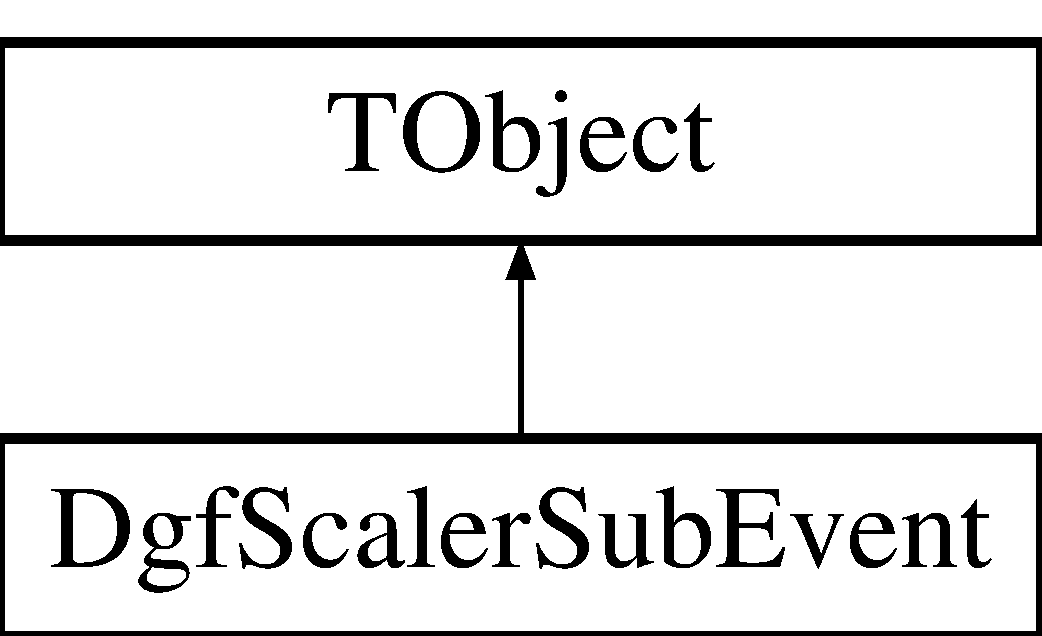
\includegraphics[height=2.000000cm]{class_dgf_scaler_sub_event}
\end{center}
\end{figure}
\subsection*{Public Member Functions}
\begin{DoxyCompactItemize}
\item 
\mbox{\Hypertarget{class_dgf_scaler_sub_event_ac65cb699d5b4871413b3c002f7b73f5a}\label{class_dgf_scaler_sub_event_ac65cb699d5b4871413b3c002f7b73f5a}} 
{\bfseries Dgf\+Scaler\+Sub\+Event} (unsigned short Number\+Of\+Dgf\+Channels)
\item 
\mbox{\Hypertarget{class_dgf_scaler_sub_event_ad0b0f669bbcc04e4b36bcdc4805f192a}\label{class_dgf_scaler_sub_event_ad0b0f669bbcc04e4b36bcdc4805f192a}} 
void {\bfseries Clear\+Evt} ()
\item 
\mbox{\Hypertarget{class_dgf_scaler_sub_event_ac922696259ea41870006d5be47874b37}\label{class_dgf_scaler_sub_event_ac922696259ea41870006d5be47874b37}} 
void {\bfseries Module\+Number} (unsigned short Dgf\+ID)
\item 
\mbox{\Hypertarget{class_dgf_scaler_sub_event_a0b7123702ce75e4a63c361a8aa6175a1}\label{class_dgf_scaler_sub_event_a0b7123702ce75e4a63c361a8aa6175a1}} 
void {\bfseries Cluster\+ID} (unsigned short Cluster\+ID)
\item 
\mbox{\Hypertarget{class_dgf_scaler_sub_event_a275332fa9b50f56b22309a49d2ee3079}\label{class_dgf_scaler_sub_event_a275332fa9b50f56b22309a49d2ee3079}} 
void {\bfseries Real\+Time} (long long time)
\item 
\mbox{\Hypertarget{class_dgf_scaler_sub_event_a597eab29b76c324a155680013ffddd8b}\label{class_dgf_scaler_sub_event_a597eab29b76c324a155680013ffddd8b}} 
void {\bfseries Run\+Time} (long long time)
\item 
\mbox{\Hypertarget{class_dgf_scaler_sub_event_ac96a965870e1ce824fab2996c2ab84fc}\label{class_dgf_scaler_sub_event_ac96a965870e1ce824fab2996c2ab84fc}} 
void {\bfseries G\+S\+L\+T\+Time} (long long time)
\item 
\mbox{\Hypertarget{class_dgf_scaler_sub_event_a62292d645d559bea309ba1016c247429}\label{class_dgf_scaler_sub_event_a62292d645d559bea309ba1016c247429}} 
void {\bfseries Number\+Of\+Events} (unsigned short numberofevents)
\item 
\mbox{\Hypertarget{class_dgf_scaler_sub_event_ab1b1268e16fc5e7b425fd99becb00c01}\label{class_dgf_scaler_sub_event_ab1b1268e16fc5e7b425fd99becb00c01}} 
void {\bfseries Live\+Time} (unsigned short i, long long time)
\item 
\mbox{\Hypertarget{class_dgf_scaler_sub_event_ae5d59c7c3ad191088a7d5ba4c92b959f}\label{class_dgf_scaler_sub_event_ae5d59c7c3ad191088a7d5ba4c92b959f}} 
void {\bfseries Fast\+Peak} (unsigned short i, unsigned int fastpeak)
\item 
\mbox{\Hypertarget{class_dgf_scaler_sub_event_a913e196c9dd4829d8bea5db881e240f7}\label{class_dgf_scaler_sub_event_a913e196c9dd4829d8bea5db881e240f7}} 
unsigned short {\bfseries Module\+Number} ()
\item 
\mbox{\Hypertarget{class_dgf_scaler_sub_event_ad481d1073428e20f69f7bb8d099b3bed}\label{class_dgf_scaler_sub_event_ad481d1073428e20f69f7bb8d099b3bed}} 
unsigned short {\bfseries Cluster\+ID} ()
\item 
\mbox{\Hypertarget{class_dgf_scaler_sub_event_a7b9076a625781dd2e3456e910c2c3239}\label{class_dgf_scaler_sub_event_a7b9076a625781dd2e3456e910c2c3239}} 
long long {\bfseries Real\+Time} ()
\item 
\mbox{\Hypertarget{class_dgf_scaler_sub_event_aeb5d3d6d053b49df431e5544ddeacdba}\label{class_dgf_scaler_sub_event_aeb5d3d6d053b49df431e5544ddeacdba}} 
long long {\bfseries Run\+Time} ()
\item 
\mbox{\Hypertarget{class_dgf_scaler_sub_event_a7684a4958881cff43c94835e34658f3b}\label{class_dgf_scaler_sub_event_a7684a4958881cff43c94835e34658f3b}} 
long long {\bfseries G\+S\+L\+T\+Time} ()
\item 
\mbox{\Hypertarget{class_dgf_scaler_sub_event_abba61fa31c82f03fcbddaaaf2e8360cc}\label{class_dgf_scaler_sub_event_abba61fa31c82f03fcbddaaaf2e8360cc}} 
unsigned short {\bfseries Number\+Of\+Events} ()
\item 
\mbox{\Hypertarget{class_dgf_scaler_sub_event_a1a3b59c0babb769e553008f0d1ff3af6}\label{class_dgf_scaler_sub_event_a1a3b59c0babb769e553008f0d1ff3af6}} 
long long {\bfseries Live\+Time} (unsigned short i)
\item 
\mbox{\Hypertarget{class_dgf_scaler_sub_event_a2d086ff6df7007e8eb1c645e9ddb5f85}\label{class_dgf_scaler_sub_event_a2d086ff6df7007e8eb1c645e9ddb5f85}} 
int {\bfseries Fast\+Peak} (unsigned short i)
\end{DoxyCompactItemize}
\subsection*{Protected Attributes}
\begin{DoxyCompactItemize}
\item 
\mbox{\Hypertarget{class_dgf_scaler_sub_event_a86dbc7481d266b668799d198807df991}\label{class_dgf_scaler_sub_event_a86dbc7481d266b668799d198807df991}} 
unsigned short {\bfseries f\+Module\+Number}
\item 
\mbox{\Hypertarget{class_dgf_scaler_sub_event_a308d5787aeb511ce698e021d69fa8d46}\label{class_dgf_scaler_sub_event_a308d5787aeb511ce698e021d69fa8d46}} 
unsigned short {\bfseries f\+Cluster\+ID}
\item 
\mbox{\Hypertarget{class_dgf_scaler_sub_event_aa459f724ff8a6621d2ce35bb8d9ac971}\label{class_dgf_scaler_sub_event_aa459f724ff8a6621d2ce35bb8d9ac971}} 
long long {\bfseries f\+Real\+Time}
\item 
\mbox{\Hypertarget{class_dgf_scaler_sub_event_a2d9ebb7063c5b6ad3beabedc58a2d4ef}\label{class_dgf_scaler_sub_event_a2d9ebb7063c5b6ad3beabedc58a2d4ef}} 
long long {\bfseries f\+Run\+Time}
\item 
\mbox{\Hypertarget{class_dgf_scaler_sub_event_aa3de3cbc37314d07172d9899e9b2951b}\label{class_dgf_scaler_sub_event_aa3de3cbc37314d07172d9899e9b2951b}} 
long long {\bfseries f\+G\+S\+L\+T\+Time}
\item 
\mbox{\Hypertarget{class_dgf_scaler_sub_event_afbbc4fdf75ad471453e0bd8930286aae}\label{class_dgf_scaler_sub_event_afbbc4fdf75ad471453e0bd8930286aae}} 
unsigned short {\bfseries f\+Number\+Of\+Events}
\item 
\mbox{\Hypertarget{class_dgf_scaler_sub_event_a7433bbc94024bb171af20d2b98658686}\label{class_dgf_scaler_sub_event_a7433bbc94024bb171af20d2b98658686}} 
vector$<$ long long $>$ {\bfseries f\+Live\+Time}
\item 
\mbox{\Hypertarget{class_dgf_scaler_sub_event_a5847eac857f67c4add3c15a7b2bb890d}\label{class_dgf_scaler_sub_event_a5847eac857f67c4add3c15a7b2bb890d}} 
vector$<$ int $>$ {\bfseries f\+Fast\+Peak}
\item 
\mbox{\Hypertarget{class_dgf_scaler_sub_event_a2deb4d871695699aac992b4179881137}\label{class_dgf_scaler_sub_event_a2deb4d871695699aac992b4179881137}} 
unsigned short {\bfseries f\+Number\+Of\+Dgf\+Channels}
\end{DoxyCompactItemize}


The documentation for this class was generated from the following files\+:\begin{DoxyCompactItemize}
\item 
Med\+To\+Root/Sub\+Events.\+hh\item 
Med\+To\+Root/Sub\+Events.\+cc\end{DoxyCompactItemize}

\hypertarget{class_dgf_sub_event}{}\section{Dgf\+Sub\+Event Class Reference}
\label{class_dgf_sub_event}\index{Dgf\+Sub\+Event@{Dgf\+Sub\+Event}}
Inheritance diagram for Dgf\+Sub\+Event\+:\begin{figure}[H]
\begin{center}
\leavevmode
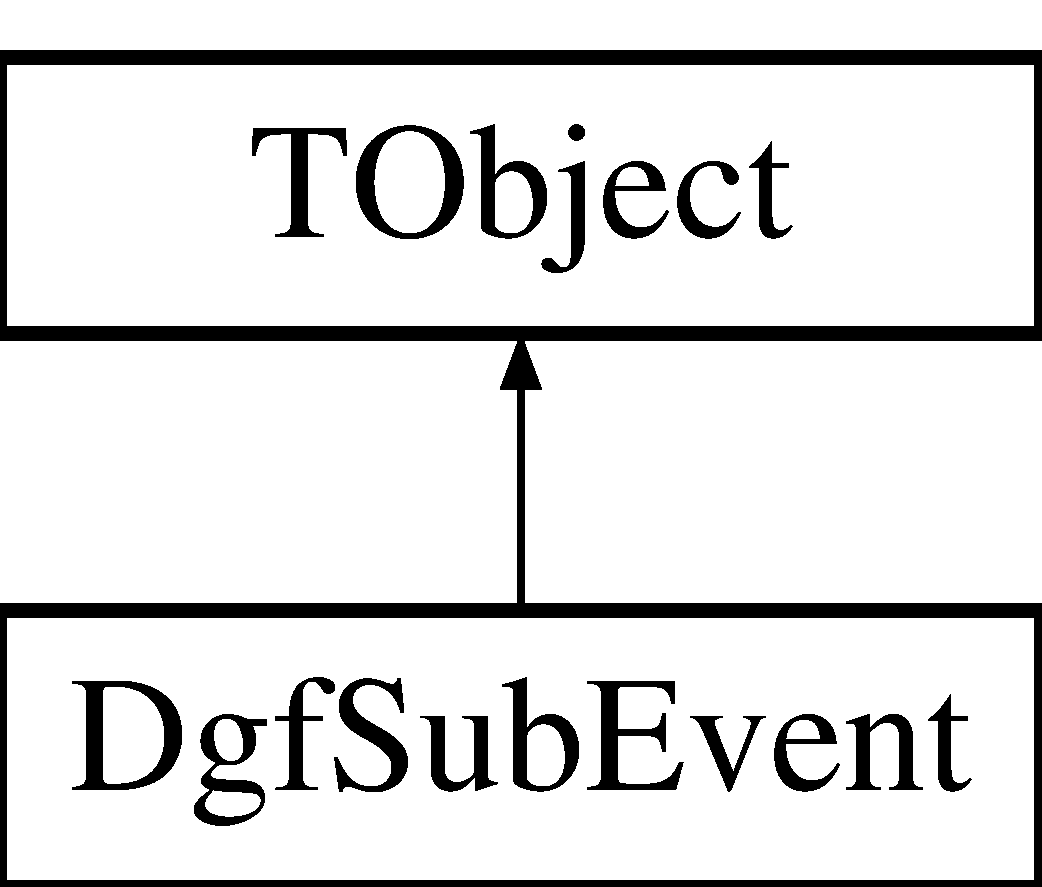
\includegraphics[height=2.000000cm]{class_dgf_sub_event}
\end{center}
\end{figure}
\subsection*{Public Member Functions}
\begin{DoxyCompactItemize}
\item 
\mbox{\Hypertarget{class_dgf_sub_event_a46977843cc3254ae9c129cf044b9a140}\label{class_dgf_sub_event_a46977843cc3254ae9c129cf044b9a140}} 
void {\bfseries Clear\+Evt} ()
\item 
\mbox{\Hypertarget{class_dgf_sub_event_a57465895ade7d2bd229d7c4b6eac28fe}\label{class_dgf_sub_event_a57465895ade7d2bd229d7c4b6eac28fe}} 
void {\bfseries Set\+Hit\+Pattern} (unsigned short hit\+Pattern)
\item 
\mbox{\Hypertarget{class_dgf_sub_event_ae7733bc6e848b1f87add491e3e4139f2}\label{class_dgf_sub_event_ae7733bc6e848b1f87add491e3e4139f2}} 
void {\bfseries Set\+Event\+Time} (unsigned short Run\+Time, unsigned short Event\+Time\+High, unsigned short Event\+Time\+Low)
\item 
\mbox{\Hypertarget{class_dgf_sub_event_afbfad40671d380b51f11e920ba2bb109}\label{class_dgf_sub_event_afbfad40671d380b51f11e920ba2bb109}} 
void {\bfseries Set\+Fast\+Trigger\+Time} (unsigned short channel\+Number, unsigned short fast\+Trigger\+Time)
\item 
\mbox{\Hypertarget{class_dgf_sub_event_a2f301efaff91959dae2a3b4d015b8cd5}\label{class_dgf_sub_event_a2f301efaff91959dae2a3b4d015b8cd5}} 
void {\bfseries Set\+Energy} (unsigned short channel\+Number, unsigned short energy)
\item 
\mbox{\Hypertarget{class_dgf_sub_event_a09387034596827f924bce4a4aa84a8be}\label{class_dgf_sub_event_a09387034596827f924bce4a4aa84a8be}} 
void {\bfseries Set\+Long\+Fast\+Trigger\+Time} (unsigned short channel\+Number, unsigned short Run\+Time, unsigned short Event\+Time\+High, unsigned short Event\+Time\+Low)
\item 
\mbox{\Hypertarget{class_dgf_sub_event_a5dd58fb29bb11c8870ef8f275024a995}\label{class_dgf_sub_event_a5dd58fb29bb11c8870ef8f275024a995}} 
void {\bfseries Set\+User\+Values} (unsigned short $\ast$\&q, unsigned short channel\+Number)
\item 
\mbox{\Hypertarget{class_dgf_sub_event_a19d751e8ab22da36113ba864b28b425e}\label{class_dgf_sub_event_a19d751e8ab22da36113ba864b28b425e}} 
unsigned short {\bfseries Get\+Hit\+Pattern} ()
\item 
\mbox{\Hypertarget{class_dgf_sub_event_adc8e12fe656b4d63ab2b6800a04eeb7c}\label{class_dgf_sub_event_adc8e12fe656b4d63ab2b6800a04eeb7c}} 
unsigned short {\bfseries Get\+Event\+Time} ()
\item 
\mbox{\Hypertarget{class_dgf_sub_event_af06c641fb0dabab29be0b8572aec5740}\label{class_dgf_sub_event_af06c641fb0dabab29be0b8572aec5740}} 
unsigned short {\bfseries Get\+Fast\+Trigger\+Time} (unsigned short channel\+Number)
\item 
\mbox{\Hypertarget{class_dgf_sub_event_a19e2d8959779de9f82c2e69225b9696f}\label{class_dgf_sub_event_a19e2d8959779de9f82c2e69225b9696f}} 
unsigned short {\bfseries Get\+Energy} (unsigned short channel\+Number)
\item 
\mbox{\Hypertarget{class_dgf_sub_event_a48cd67e00b26bc1b707407f0b505a30c}\label{class_dgf_sub_event_a48cd67e00b26bc1b707407f0b505a30c}} 
unsigned short {\bfseries Get\+Number\+Of\+Channels} ()
\item 
\mbox{\Hypertarget{class_dgf_sub_event_ad1b9df7d345fd7dddbeae27fc603b7e2}\label{class_dgf_sub_event_ad1b9df7d345fd7dddbeae27fc603b7e2}} 
long long {\bfseries Get\+Long\+Fast\+Trigger\+Time} (unsigned short channel\+Number)
\item 
\mbox{\Hypertarget{class_dgf_sub_event_a44c415993ed2496e6facfd29536df744}\label{class_dgf_sub_event_a44c415993ed2496e6facfd29536df744}} 
void {\bfseries Get\+User\+Values} (unsigned short channel\+Number, unsigned short $\ast$user\+Values)
\end{DoxyCompactItemize}
\subsection*{Protected Attributes}
\begin{DoxyCompactItemize}
\item 
\mbox{\Hypertarget{class_dgf_sub_event_af2f6acbebcc14dd9a790cf88a44a35a4}\label{class_dgf_sub_event_af2f6acbebcc14dd9a790cf88a44a35a4}} 
unsigned short {\bfseries Hit\+Pattern}
\item 
\mbox{\Hypertarget{class_dgf_sub_event_aedcb285d2a8853ac8dd0de4983a82e18}\label{class_dgf_sub_event_aedcb285d2a8853ac8dd0de4983a82e18}} 
long long {\bfseries Event\+Time}
\item 
\mbox{\Hypertarget{class_dgf_sub_event_a73fc042eb429ad9232811351cc0059c5}\label{class_dgf_sub_event_a73fc042eb429ad9232811351cc0059c5}} 
unsigned short {\bfseries Energy} \mbox{[}Number\+Of\+Channels\mbox{]}
\item 
\mbox{\Hypertarget{class_dgf_sub_event_a55acb5f1b72f274f7201d33df90620e5}\label{class_dgf_sub_event_a55acb5f1b72f274f7201d33df90620e5}} 
unsigned short {\bfseries Fast\+Trigger\+Time} \mbox{[}Number\+Of\+Channels\mbox{]}
\item 
\mbox{\Hypertarget{class_dgf_sub_event_a1a4328e7ef711bd75cd82a89b6fddad5}\label{class_dgf_sub_event_a1a4328e7ef711bd75cd82a89b6fddad5}} 
long long {\bfseries Long\+Fast\+Trigger\+Time} \mbox{[}Number\+Of\+Channels\mbox{]}
\item 
\mbox{\Hypertarget{class_dgf_sub_event_aaa57b5de7ab6aedd46a9f1486d37719c}\label{class_dgf_sub_event_aaa57b5de7ab6aedd46a9f1486d37719c}} 
unsigned short {\bfseries User\+Values} \mbox{[}Number\+Of\+Channels\mbox{]}\mbox{[}Number\+Of\+User\+Values\mbox{]}
\end{DoxyCompactItemize}
\subsection*{Friends}
\begin{DoxyCompactItemize}
\item 
\mbox{\Hypertarget{class_dgf_sub_event_a98fb82e2308f57cabcdf001424381c3e}\label{class_dgf_sub_event_a98fb82e2308f57cabcdf001424381c3e}} 
ostream \& {\bfseries operator$<$$<$} (ostream \&, const \hyperlink{class_dgf_sub_event}{Dgf\+Sub\+Event} \&)
\end{DoxyCompactItemize}


The documentation for this class was generated from the following files\+:\begin{DoxyCompactItemize}
\item 
Med\+To\+Root/Sub\+Events.\+hh\item 
Med\+To\+Root/Sub\+Events.\+cc\end{DoxyCompactItemize}

\hypertarget{classdoppler}{}\section{doppler Class Reference}
\label{classdoppler}\index{doppler@{doppler}}


A class for performing all aspects of the Doppler correction.  




{\ttfamily \#include $<$doppler.\+hh$>$}

Inheritance diagram for doppler\+:\begin{figure}[H]
\begin{center}
\leavevmode
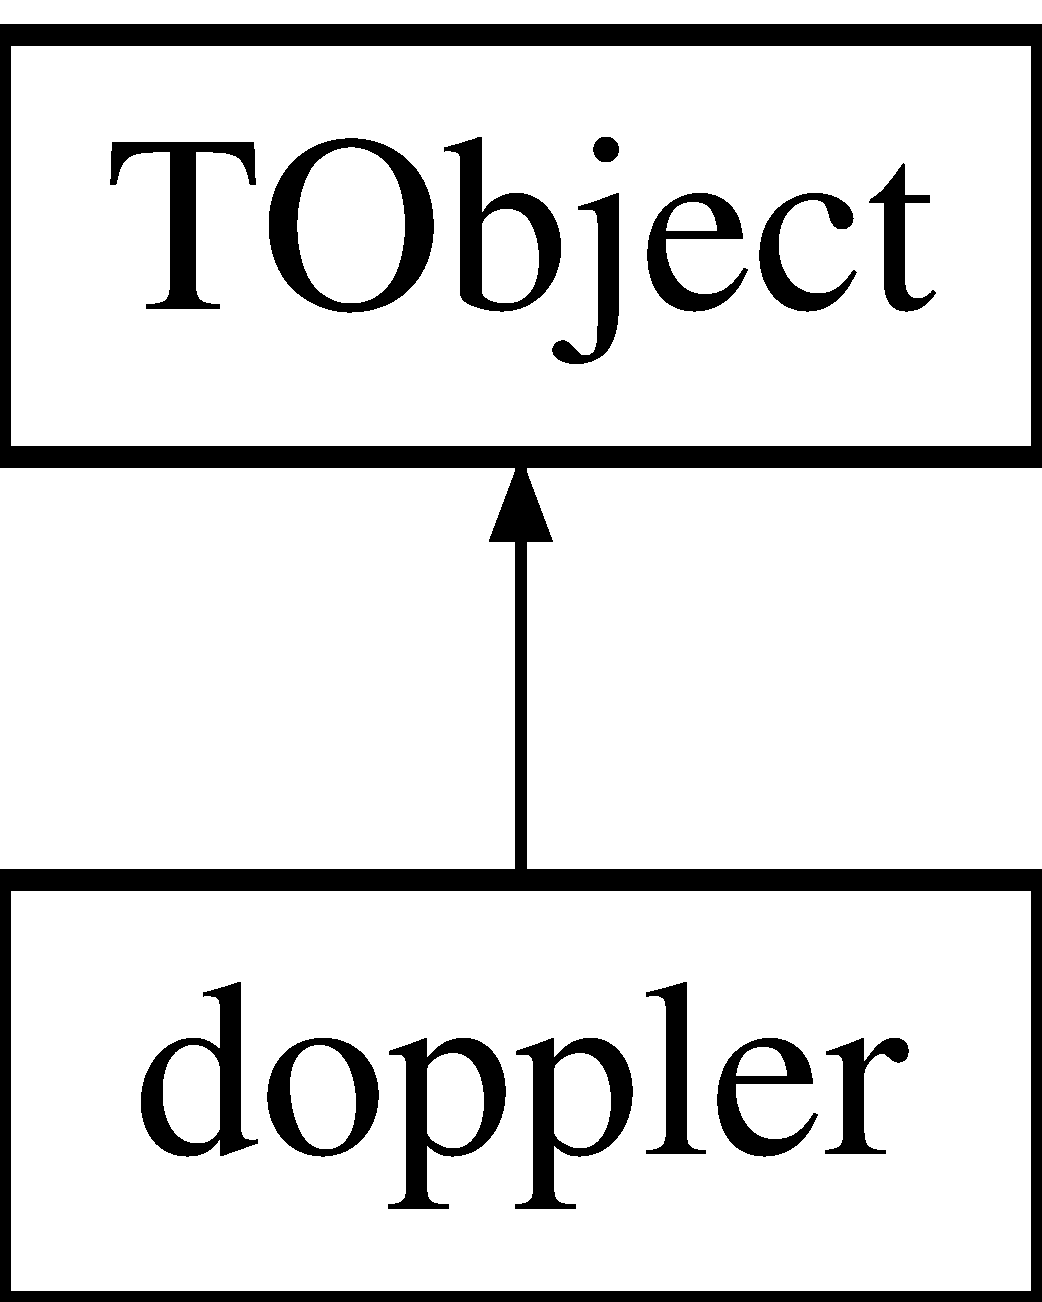
\includegraphics[height=2.000000cm]{classdoppler}
\end{center}
\end{figure}
\subsection*{Public Member Functions}
\begin{DoxyCompactItemize}
\item 
void \hyperlink{classdoppler_ac628277148db1641251745f86ba3dc52}{Exp\+Defs} (int Zb\+\_\+, float Ab\+\_\+, int Zt\+\_\+, float At\+\_\+, float Eb\+\_\+, float Ex\+\_\+, float thick\+\_\+, float depth\+\_\+, float cddist\+\_\+, float cdoffset\+\_\+, float deadlayer\+\_\+, float contaminant\+\_\+, float spededist\+\_\+, T\+CutG $\ast$Bcut\+\_\+, T\+CutG $\ast$Tcut\+\_\+)
\item 
int \hyperlink{classdoppler_aa3debb227d73f7cdea5b02e4c202cb19}{Cut} (float P\+En, float anno, int quad)
\item 
int \hyperlink{classdoppler_a52f116733da78465469a75ced66915a8}{Cut\+\_\+2p} (float P\+En1, float anno1, int quad1, float P\+En2, float anno2, int quad2)
\item 
bool \hyperlink{classdoppler_a56df9f9384f469385458193754c743c9}{Cut\+G\+\_\+en2hit} (float B\+En, float T\+En)
\item 
int \hyperlink{classdoppler_a29e9a1565d90df9f5d9deef05cdbf53c}{Get\+Zb} ()
\item 
int \hyperlink{classdoppler_ac0587ca2b963edec86d17dd6dac024ce}{Get\+Zt} ()
\item 
float \hyperlink{classdoppler_ac3cde63421ff794992231027245ceced}{Get\+Ab} ()
\item 
float \hyperlink{classdoppler_a72bb0dc1707c0f2bf4b978caf06f2cf1}{Get\+At} ()
\item 
float \hyperlink{classdoppler_ac7725720fab82af5a5a6f02041bc9483}{Get\+C\+D\+Offset} ()
\item 
float \hyperlink{classdoppler_a2c1aef6db4ad3fc0c98e91d995992706}{Get\+C\+D\+Dead\+Layer} ()
\item 
float \hyperlink{classdoppler_ae45abdba9f375009cdeba5ac81d7b32c}{Get\+Spede\+Dist} ()
\item 
float \hyperlink{classdoppler_a1415bdb47dbb9d5eba7f14a64bd3693e}{Get\+P\+Th} (float anno)
\item 
float \hyperlink{classdoppler_a0f57a8f4a8c369c14d52e62dd3833f2e}{Get\+P\+Phi} (int quad, int seg)
\item 
float \hyperlink{classdoppler_ac8f059cc77214a954be534a85c748a3c}{Get\+P\+Phi} (int quad, int seg, float offset)
\item 
float \hyperlink{classdoppler_a7865dcf92a6b18d23cb48e9e624e505b}{Get\+T\+Th} (float Banno, float B\+En)
\item 
float \hyperlink{classdoppler_ac834d80156ae80009b508ae41fedde3d}{Get\+B\+Th} (float Tanno)
\item 
float \hyperlink{classdoppler_a7c3afd05ed9ddb8c5bedc0de905acd0b}{Get\+Q\+Phi} (int quad, int seg)
\item 
float \hyperlink{classdoppler_a31a09afe8920dc1302162ec8e0be9302}{Get\+T\+En} (float B\+En, float Banno)
\item 
float \hyperlink{classdoppler_a182d987ddc6db4a8b8e7f7821bda3846}{Get\+B\+En} (float T\+En, float Tanno)
\item 
float \hyperlink{classdoppler_a64570ec784dabd6e17cf836489450527}{Get\+E\+Loss} (float Ei, float dist, int opt, string combo)
\item 
float \hyperlink{classdoppler_a6dca381f91f2267abefadd62cf66f69f}{Gamma\+Ang} (float P\+Th, float P\+Phi, float G\+Th, float G\+Phi)
\item 
float \hyperlink{classdoppler_a28eb084d224fdb58fda1d6f6c61dd232}{Beta} (float Ek, float m)
\item 
float \hyperlink{classdoppler_a7f08d93d2bfa269f8c22ac71b604b09a}{DC} (float P\+En, float P\+Th, float P\+Phi, float G\+Th, float G\+Phi, float A)
\item 
float \hyperlink{classdoppler_ad8387753c2288d464b64579a23d3bc4e}{D\+C\+\_\+elec} (float een, float P\+En, float P\+Th, float P\+Phi, float G\+Th, float G\+Phi, float A)
\item 
bool \hyperlink{classdoppler_ad91321c9c9220fff724e5e0982e1a8b8}{stoppingpowers} (bool BT, bool TT, bool BA, bool TA, bool BC, bool TC)
\item 
bool \hyperlink{classdoppler_a4be762591578e28f8e9d646475ca943a}{stoppingpowers} (string opt)
\item 
\mbox{\Hypertarget{classdoppler_a68d168fdd3cb3edeb4a015aeaf0d3391}\label{classdoppler_a68d168fdd3cb3edeb4a015aeaf0d3391}} 
float {\bfseries u\+\_\+mass} ()
\item 
\mbox{\Hypertarget{classdoppler_ab05f91fbb4af54aef0bf595bd1803be8}\label{classdoppler_ab05f91fbb4af54aef0bf595bd1803be8}} 
void {\bfseries Exp\+Defs} (int Zb\+\_\+, int Ab\+\_\+, int Zt\+\_\+, int At\+\_\+, float Eb\+\_\+, float Ex\+\_\+, float thick\+\_\+, float depth\+\_\+, float cddist\+\_\+, float cdoffset\+\_\+, float deadlayer\+\_\+, float plunger\+\_\+, T\+CutG $\ast$Bcut\+\_\+, T\+CutG $\ast$Tcut\+\_\+)
\item 
\mbox{\Hypertarget{classdoppler_aa3debb227d73f7cdea5b02e4c202cb19}\label{classdoppler_aa3debb227d73f7cdea5b02e4c202cb19}} 
int {\bfseries Cut} (float P\+En, float anno, int quad)
\item 
\mbox{\Hypertarget{classdoppler_a52f116733da78465469a75ced66915a8}\label{classdoppler_a52f116733da78465469a75ced66915a8}} 
int {\bfseries Cut\+\_\+2p} (float P\+En1, float anno1, int quad1, float P\+En2, float anno2, int quad2)
\item 
\mbox{\Hypertarget{classdoppler_a56df9f9384f469385458193754c743c9}\label{classdoppler_a56df9f9384f469385458193754c743c9}} 
bool {\bfseries Cut\+G\+\_\+en2hit} (float B\+En, float T\+En)
\item 
\mbox{\Hypertarget{classdoppler_a29e9a1565d90df9f5d9deef05cdbf53c}\label{classdoppler_a29e9a1565d90df9f5d9deef05cdbf53c}} 
int {\bfseries Get\+Zb} ()
\item 
\mbox{\Hypertarget{classdoppler_ac3cde63421ff794992231027245ceced}\label{classdoppler_ac3cde63421ff794992231027245ceced}} 
int {\bfseries Get\+Ab} ()
\item 
\mbox{\Hypertarget{classdoppler_ac0587ca2b963edec86d17dd6dac024ce}\label{classdoppler_ac0587ca2b963edec86d17dd6dac024ce}} 
int {\bfseries Get\+Zt} ()
\item 
\mbox{\Hypertarget{classdoppler_a72bb0dc1707c0f2bf4b978caf06f2cf1}\label{classdoppler_a72bb0dc1707c0f2bf4b978caf06f2cf1}} 
int {\bfseries Get\+At} ()
\item 
\mbox{\Hypertarget{classdoppler_ac7725720fab82af5a5a6f02041bc9483}\label{classdoppler_ac7725720fab82af5a5a6f02041bc9483}} 
float {\bfseries Get\+C\+D\+Offset} ()
\item 
\mbox{\Hypertarget{classdoppler_a2c1aef6db4ad3fc0c98e91d995992706}\label{classdoppler_a2c1aef6db4ad3fc0c98e91d995992706}} 
float {\bfseries Get\+C\+D\+Dead\+Layer} ()
\item 
\mbox{\Hypertarget{classdoppler_accc85c5ab5f322ec2c321f7653ccc40f}\label{classdoppler_accc85c5ab5f322ec2c321f7653ccc40f}} 
float {\bfseries Get\+Plunger\+Dist} ()
\item 
\mbox{\Hypertarget{classdoppler_a1415bdb47dbb9d5eba7f14a64bd3693e}\label{classdoppler_a1415bdb47dbb9d5eba7f14a64bd3693e}} 
float {\bfseries Get\+P\+Th} (float anno)
\item 
\mbox{\Hypertarget{classdoppler_a0f57a8f4a8c369c14d52e62dd3833f2e}\label{classdoppler_a0f57a8f4a8c369c14d52e62dd3833f2e}} 
float {\bfseries Get\+P\+Phi} (int quad, int seg)
\item 
\mbox{\Hypertarget{classdoppler_ac8f059cc77214a954be534a85c748a3c}\label{classdoppler_ac8f059cc77214a954be534a85c748a3c}} 
float {\bfseries Get\+P\+Phi} (int quad, int seg, float offset)
\item 
\mbox{\Hypertarget{classdoppler_a7865dcf92a6b18d23cb48e9e624e505b}\label{classdoppler_a7865dcf92a6b18d23cb48e9e624e505b}} 
float {\bfseries Get\+T\+Th} (float Banno, float B\+En)
\item 
\mbox{\Hypertarget{classdoppler_ac834d80156ae80009b508ae41fedde3d}\label{classdoppler_ac834d80156ae80009b508ae41fedde3d}} 
float {\bfseries Get\+B\+Th} (float Tanno)
\item 
\mbox{\Hypertarget{classdoppler_a7c3afd05ed9ddb8c5bedc0de905acd0b}\label{classdoppler_a7c3afd05ed9ddb8c5bedc0de905acd0b}} 
float {\bfseries Get\+Q\+Phi} (int quad, int seg)
\item 
\mbox{\Hypertarget{classdoppler_a31a09afe8920dc1302162ec8e0be9302}\label{classdoppler_a31a09afe8920dc1302162ec8e0be9302}} 
float {\bfseries Get\+T\+En} (float B\+En, float Banno)
\item 
\mbox{\Hypertarget{classdoppler_a182d987ddc6db4a8b8e7f7821bda3846}\label{classdoppler_a182d987ddc6db4a8b8e7f7821bda3846}} 
float {\bfseries Get\+B\+En} (float T\+En, float Tanno)
\item 
\mbox{\Hypertarget{classdoppler_a64570ec784dabd6e17cf836489450527}\label{classdoppler_a64570ec784dabd6e17cf836489450527}} 
float {\bfseries Get\+E\+Loss} (float Ei, float dist, int opt, string combo)
\item 
\mbox{\Hypertarget{classdoppler_a6dca381f91f2267abefadd62cf66f69f}\label{classdoppler_a6dca381f91f2267abefadd62cf66f69f}} 
float {\bfseries Gamma\+Ang} (float P\+Th, float P\+Phi, float G\+Th, float G\+Phi)
\item 
\mbox{\Hypertarget{classdoppler_a7f08d93d2bfa269f8c22ac71b604b09a}\label{classdoppler_a7f08d93d2bfa269f8c22ac71b604b09a}} 
float {\bfseries DC} (float P\+En, float P\+Th, float P\+Phi, float G\+Th, float G\+Phi, float A)
\item 
\mbox{\Hypertarget{classdoppler_af3fe2bbd813b2c84fc79b156879205fd}\label{classdoppler_af3fe2bbd813b2c84fc79b156879205fd}} 
bool {\bfseries stoppingpowers} (bool BT, bool TT, bool BS, bool TS)
\item 
\mbox{\Hypertarget{classdoppler_a4be762591578e28f8e9d646475ca943a}\label{classdoppler_a4be762591578e28f8e9d646475ca943a}} 
bool {\bfseries stoppingpowers} (string opt)
\end{DoxyCompactItemize}
\subsection*{Static Public Member Functions}
\begin{DoxyCompactItemize}
\item 
static string \hyperlink{classdoppler_a100e363bf80b5371baebb89bbf60b824}{convert\+Int} (int number)
\item 
static string \hyperlink{classdoppler_a0fa8eec8989c81e59ecfb8e09140020c}{convert\+Float} (float number)
\item 
\mbox{\Hypertarget{classdoppler_ae9020810d4d7235eacf2b875c52172f8}\label{classdoppler_ae9020810d4d7235eacf2b875c52172f8}} 
static Int\+\_\+t {\bfseries Cut} (Double\+\_\+t P\+En, Double\+\_\+t anno, Int\+\_\+t quad)
\item 
\mbox{\Hypertarget{classdoppler_add35c6b42292a11a41d4ef055fbf231a}\label{classdoppler_add35c6b42292a11a41d4ef055fbf231a}} 
static Int\+\_\+t {\bfseries Cut\+\_\+2p} (Double\+\_\+t P\+En1, Double\+\_\+t anno1, Int\+\_\+t quad1, Double\+\_\+t P\+En2, Double\+\_\+t anno2, Int\+\_\+t quad2)
\item 
\mbox{\Hypertarget{classdoppler_a39beed8120adbda7dffdeb4e17e986c2}\label{classdoppler_a39beed8120adbda7dffdeb4e17e986c2}} 
static bool {\bfseries Cut\+G\+\_\+en2hit} (double B\+En, double T\+En)
\item 
\mbox{\Hypertarget{classdoppler_a3dca88d6ac6d2c411ca26883eb10787a}\label{classdoppler_a3dca88d6ac6d2c411ca26883eb10787a}} 
static Double\+\_\+t {\bfseries Get\+Tar\+Dist} ()
\item 
\mbox{\Hypertarget{classdoppler_a562426907365a2c4c56fc393264394a4}\label{classdoppler_a562426907365a2c4c56fc393264394a4}} 
static Double\+\_\+t {\bfseries Get\+P\+Th} (Double\+\_\+t anno)
\item 
\mbox{\Hypertarget{classdoppler_ac9cc83b2b22576320980abab50710909}\label{classdoppler_ac9cc83b2b22576320980abab50710909}} 
static Double\+\_\+t {\bfseries Get\+P\+Phi} (Int\+\_\+t quad, Int\+\_\+t seg, float offset=242.\+6)
\item 
\mbox{\Hypertarget{classdoppler_a87a75dbf49952fa574b80e6a991d0286}\label{classdoppler_a87a75dbf49952fa574b80e6a991d0286}} 
static Double\+\_\+t {\bfseries Get\+T\+Th} (Double\+\_\+t Banno, Double\+\_\+t B\+En)
\item 
\mbox{\Hypertarget{classdoppler_a42de1470ae67fefdb3ca1ea1f4d0f326}\label{classdoppler_a42de1470ae67fefdb3ca1ea1f4d0f326}} 
static Double\+\_\+t {\bfseries Get\+B\+Th} (Double\+\_\+t Tanno)
\item 
\mbox{\Hypertarget{classdoppler_ab8fcb952d529bbd30d147bf34f159c73}\label{classdoppler_ab8fcb952d529bbd30d147bf34f159c73}} 
static Double\+\_\+t {\bfseries Get\+Q\+Phi} (Int\+\_\+t quad, Int\+\_\+t seg)
\item 
\mbox{\Hypertarget{classdoppler_aec7a929023626e54c17d4c83f2a6d2c3}\label{classdoppler_aec7a929023626e54c17d4c83f2a6d2c3}} 
static Double\+\_\+t {\bfseries Get\+T\+En} (Double\+\_\+t B\+En, Double\+\_\+t Banno)
\item 
\mbox{\Hypertarget{classdoppler_ad9a413e3272258f7ad88abeb2760bdbc}\label{classdoppler_ad9a413e3272258f7ad88abeb2760bdbc}} 
static Double\+\_\+t {\bfseries Get\+B\+En} (Double\+\_\+t T\+En, Double\+\_\+t Tanno)
\item 
\mbox{\Hypertarget{classdoppler_a154716ffad9dc13095b9accdd8197e04}\label{classdoppler_a154716ffad9dc13095b9accdd8197e04}} 
static Double\+\_\+t {\bfseries Get\+E\+Loss} (Double\+\_\+t Ei, Double\+\_\+t dist, Int\+\_\+t opt, string combo)
\item 
\mbox{\Hypertarget{classdoppler_abdefc570d0519bd0e99f9a92d22707de}\label{classdoppler_abdefc570d0519bd0e99f9a92d22707de}} 
static Double\+\_\+t {\bfseries Gamma\+Ang} (Double\+\_\+t P\+Th, Double\+\_\+t P\+Phi, Double\+\_\+t G\+Th, Double\+\_\+t G\+Phi)
\item 
\mbox{\Hypertarget{classdoppler_a4eada56b71bec8f2218c6487431ed3f7}\label{classdoppler_a4eada56b71bec8f2218c6487431ed3f7}} 
static Double\+\_\+t {\bfseries DC} (Double\+\_\+t P\+En, Double\+\_\+t P\+Th, Double\+\_\+t P\+Phi, Double\+\_\+t G\+Th, Double\+\_\+t G\+Phi, Double\+\_\+t A)
\item 
\mbox{\Hypertarget{classdoppler_a2d42bc47c077b472a9cbdd500d8092bc}\label{classdoppler_a2d42bc47c077b472a9cbdd500d8092bc}} 
static Double\+\_\+t {\bfseries D\+C\+\_\+elec} (double een, double P\+En, double P\+Th, double P\+Phi, double G\+Th, double G\+Phi, double A)
\item 
\mbox{\Hypertarget{classdoppler_add47e854c8b41d33ff6054c8daf0d163}\label{classdoppler_add47e854c8b41d33ff6054c8daf0d163}} 
static bool {\bfseries stoppingpowers} (Int\+\_\+t Zp, Int\+\_\+t Zt, Double\+\_\+t Ap, Double\+\_\+t At, string opt)
\item 
\mbox{\Hypertarget{classdoppler_a34a6c6112ce5e719a13a722353c8214f}\label{classdoppler_a34a6c6112ce5e719a13a722353c8214f}} 
static string {\bfseries convert\+Int} (int number)
\item 
\mbox{\Hypertarget{classdoppler_a3148106ce3d9d4861c505dab61ed7aae}\label{classdoppler_a3148106ce3d9d4861c505dab61ed7aae}} 
static string {\bfseries convert\+Float} (float number)
\item 
\mbox{\Hypertarget{classdoppler_a34a6c6112ce5e719a13a722353c8214f}\label{classdoppler_a34a6c6112ce5e719a13a722353c8214f}} 
static string {\bfseries convert\+Int} (int number)
\item 
\mbox{\Hypertarget{classdoppler_a3148106ce3d9d4861c505dab61ed7aae}\label{classdoppler_a3148106ce3d9d4861c505dab61ed7aae}} 
static string {\bfseries convert\+Float} (float number)
\end{DoxyCompactItemize}
\subsection*{Private Member Functions}
\begin{DoxyCompactItemize}
\item 
\mbox{\Hypertarget{classdoppler_ade7546707b0924034fea20592ea8be3f}\label{classdoppler_ade7546707b0924034fea20592ea8be3f}} 
{\bfseries Class\+Def} (\hyperlink{classdoppler}{doppler}, 1)
\item 
\mbox{\Hypertarget{classdoppler_ade7546707b0924034fea20592ea8be3f}\label{classdoppler_ade7546707b0924034fea20592ea8be3f}} 
{\bfseries Class\+Def} (\hyperlink{classdoppler}{doppler}, 1)
\item 
\mbox{\Hypertarget{classdoppler_ade7546707b0924034fea20592ea8be3f}\label{classdoppler_ade7546707b0924034fea20592ea8be3f}} 
{\bfseries Class\+Def} (\hyperlink{classdoppler}{doppler}, 1)
\end{DoxyCompactItemize}
\subsection*{Static Private Member Functions}
\begin{DoxyCompactItemize}
\item 
\mbox{\Hypertarget{classdoppler_a796802036480843f258b284f5832bd98}\label{classdoppler_a796802036480843f258b284f5832bd98}} 
static double {\bfseries S\+P\+\_\+function} (double $\ast$x, double $\ast$par)
\item 
\mbox{\Hypertarget{classdoppler_a624531c02ac2c5bbb07755047b36970a}\label{classdoppler_a624531c02ac2c5bbb07755047b36970a}} 
static double {\bfseries S\+P\+\_\+function} (double $\ast$x, double $\ast$par)
\end{DoxyCompactItemize}
\subsection*{Private Attributes}
\begin{DoxyCompactItemize}
\item 
\mbox{\Hypertarget{classdoppler_a68aa6852863cc61aac4b48232984d9e3}\label{classdoppler_a68aa6852863cc61aac4b48232984d9e3}} 
T\+Graph $\ast$ {\bfseries g\+SP} \mbox{[}6\mbox{]}
\item 
\mbox{\Hypertarget{classdoppler_a9d471fcad9598fd2ade30e33fa975a68}\label{classdoppler_a9d471fcad9598fd2ade30e33fa975a68}} 
int {\bfseries Zb}
\item 
\mbox{\Hypertarget{classdoppler_af8a5a56a1df23ebbad07fc02dc769301}\label{classdoppler_af8a5a56a1df23ebbad07fc02dc769301}} 
int {\bfseries Zt}
\item 
\mbox{\Hypertarget{classdoppler_a5cade73bdf88628d2249fe132fafa09d}\label{classdoppler_a5cade73bdf88628d2249fe132fafa09d}} 
float {\bfseries Ab}
\item 
\mbox{\Hypertarget{classdoppler_a74c6dbe49c10b46c6a7359d63bb2de70}\label{classdoppler_a74c6dbe49c10b46c6a7359d63bb2de70}} 
float {\bfseries At}
\item 
\mbox{\Hypertarget{classdoppler_a9a878a5ca9fc4137f5947bb92d7425c2}\label{classdoppler_a9a878a5ca9fc4137f5947bb92d7425c2}} 
float {\bfseries Eb}
\item 
\mbox{\Hypertarget{classdoppler_a98c25c360b741e6974ed025c4729a99e}\label{classdoppler_a98c25c360b741e6974ed025c4729a99e}} 
float {\bfseries Ex}
\item 
\mbox{\Hypertarget{classdoppler_ae033bed03e9914f81466554748fb8f52}\label{classdoppler_ae033bed03e9914f81466554748fb8f52}} 
float {\bfseries thick}
\item 
\mbox{\Hypertarget{classdoppler_ac238412e666b74f8e087841d74ba29d9}\label{classdoppler_ac238412e666b74f8e087841d74ba29d9}} 
float {\bfseries depth}
\item 
\mbox{\Hypertarget{classdoppler_ab7b2d87bd7a05a73cc01c26d76e8cd93}\label{classdoppler_ab7b2d87bd7a05a73cc01c26d76e8cd93}} 
float {\bfseries cddist}
\item 
\mbox{\Hypertarget{classdoppler_ade25af8752bc9c54cfb04a1c444f2be6}\label{classdoppler_ade25af8752bc9c54cfb04a1c444f2be6}} 
float {\bfseries cdoffset}
\item 
\mbox{\Hypertarget{classdoppler_a09bc0cdb38a83eaa1e9d1d3e34c6e5cc}\label{classdoppler_a09bc0cdb38a83eaa1e9d1d3e34c6e5cc}} 
float {\bfseries deadlayer}
\item 
\mbox{\Hypertarget{classdoppler_a9f50aca8788087aec33b5bbc17fcb136}\label{classdoppler_a9f50aca8788087aec33b5bbc17fcb136}} 
float {\bfseries contaminant}
\item 
\mbox{\Hypertarget{classdoppler_a977ce490a70aa7f4db76a6e2315ca21c}\label{classdoppler_a977ce490a70aa7f4db76a6e2315ca21c}} 
float {\bfseries spededist}
\item 
\mbox{\Hypertarget{classdoppler_af3b8c866c2e7ede2d32769cbc758fa9d}\label{classdoppler_af3b8c866c2e7ede2d32769cbc758fa9d}} 
float {\bfseries bg\+\_\+frac}
\item 
\mbox{\Hypertarget{classdoppler_a5760c500f9e7c77bc3ec325210218653}\label{classdoppler_a5760c500f9e7c77bc3ec325210218653}} 
T\+CutG $\ast$ {\bfseries Bcut}
\item 
\mbox{\Hypertarget{classdoppler_a6c9da779ddf01933a0c9c75a48abc865}\label{classdoppler_a6c9da779ddf01933a0c9c75a48abc865}} 
T\+CutG $\ast$ {\bfseries Tcut}
\item 
\mbox{\Hypertarget{classdoppler_aca9421451d063e15e77f28badad5c434}\label{classdoppler_aca9421451d063e15e77f28badad5c434}} 
int {\bfseries Ab}
\item 
\mbox{\Hypertarget{classdoppler_a5ef298f54f642ab13b249ee9d8930cd9}\label{classdoppler_a5ef298f54f642ab13b249ee9d8930cd9}} 
int {\bfseries At}
\item 
\mbox{\Hypertarget{classdoppler_adc26b8499108cb3d36d7fbf9efa7e5ed}\label{classdoppler_adc26b8499108cb3d36d7fbf9efa7e5ed}} 
float {\bfseries plunger}
\end{DoxyCompactItemize}
\subsection*{Static Private Attributes}
\begin{DoxyCompactItemize}
\item 
\mbox{\Hypertarget{classdoppler_a6b0752081184728b3b927ca03d952589}\label{classdoppler_a6b0752081184728b3b927ca03d952589}} 
static T\+Random3 {\bfseries rand} = 1
\item 
\mbox{\Hypertarget{classdoppler_aaa75d2d9cc2d380f05398fdd7c40581c}\label{classdoppler_aaa75d2d9cc2d380f05398fdd7c40581c}} 
static string {\bfseries g\+El\+Name} \mbox{[}110\mbox{]}
\item 
\mbox{\Hypertarget{classdoppler_a63d9bf44487b4d82fcc414a4d8ab4338}\label{classdoppler_a63d9bf44487b4d82fcc414a4d8ab4338}} 
static float {\bfseries gates} \mbox{[}64\mbox{]}\mbox{[}3\mbox{]}
\item 
\mbox{\Hypertarget{classdoppler_a814add11861b9c0b790103a674afae2c}\label{classdoppler_a814add11861b9c0b790103a674afae2c}} 
static double {\bfseries B\+T\+E\+Loss\+\_\+pars} \mbox{[}6\mbox{]} = \{ -\/0.\+88, 0.\+91, -\/0.\+064, -\/27., 4.\+5, -\/0.\+16 \}
\item 
\mbox{\Hypertarget{classdoppler_a3da865b4e9545e0967c9136b7e12bd96}\label{classdoppler_a3da865b4e9545e0967c9136b7e12bd96}} 
static double {\bfseries T\+T\+E\+Loss\+\_\+pars} \mbox{[}6\mbox{]} = \{ -\/0.\+88, 0.\+91, -\/0.\+064, -\/27., 4.\+5, -\/0.\+16 \}
\item 
\mbox{\Hypertarget{classdoppler_a5356d14a840882ee136903b040d70e89}\label{classdoppler_a5356d14a840882ee136903b040d70e89}} 
static double {\bfseries B\+S\+E\+Loss\+\_\+pars} \mbox{[}6\mbox{]} = \{ 3.\+6, -\/0.\+15, 0.\+010, -\/37., 6.\+1, -\/0.\+22 \}
\item 
\mbox{\Hypertarget{classdoppler_a95e5670612ee5ef760d9a35fc0093554}\label{classdoppler_a95e5670612ee5ef760d9a35fc0093554}} 
static double {\bfseries T\+S\+E\+Loss\+\_\+pars} \mbox{[}6\mbox{]} = \{ 3.\+6, -\/0.\+15, 0.\+010, -\/37., 6.\+1, -\/0.\+22 \}
\item 
\mbox{\Hypertarget{classdoppler_ae4beeefb26d1fe2552b457758fbb7e3d}\label{classdoppler_ae4beeefb26d1fe2552b457758fbb7e3d}} 
static double {\bfseries gates} \mbox{[}64\mbox{]}\mbox{[}3\mbox{]}
\end{DoxyCompactItemize}


\subsection{Detailed Description}
A class for performing all aspects of the Doppler correction. 

The doppler class has a whole suite of functions for performing the Doppler correction, including\+: calculating kinematics, energy loss, particle gating, gamma-\/ray angles, particle angles, etc. 

\subsection{Member Function Documentation}
\mbox{\Hypertarget{classdoppler_a28eb084d224fdb58fda1d6f6c61dd232}\label{classdoppler_a28eb084d224fdb58fda1d6f6c61dd232}} 
\index{doppler@{doppler}!Beta@{Beta}}
\index{Beta@{Beta}!doppler@{doppler}}
\subsubsection{\texorpdfstring{Beta()}{Beta()}}
{\footnotesize\ttfamily float doppler\+::\+Beta (\begin{DoxyParamCaption}\item[{float}]{Ek,  }\item[{float}]{m }\end{DoxyParamCaption})}

Returns beta after Taylor expansion to third order \mbox{\Hypertarget{classdoppler_a0fa8eec8989c81e59ecfb8e09140020c}\label{classdoppler_a0fa8eec8989c81e59ecfb8e09140020c}} 
\index{doppler@{doppler}!convert\+Float@{convert\+Float}}
\index{convert\+Float@{convert\+Float}!doppler@{doppler}}
\subsubsection{\texorpdfstring{convert\+Float()}{convertFloat()}}
{\footnotesize\ttfamily string doppler\+::convert\+Float (\begin{DoxyParamCaption}\item[{float}]{number }\end{DoxyParamCaption})\hspace{0.3cm}{\ttfamily [static]}}

Convert an float into a string \mbox{\Hypertarget{classdoppler_a100e363bf80b5371baebb89bbf60b824}\label{classdoppler_a100e363bf80b5371baebb89bbf60b824}} 
\index{doppler@{doppler}!convert\+Int@{convert\+Int}}
\index{convert\+Int@{convert\+Int}!doppler@{doppler}}
\subsubsection{\texorpdfstring{convert\+Int()}{convertInt()}}
{\footnotesize\ttfamily string doppler\+::convert\+Int (\begin{DoxyParamCaption}\item[{int}]{number }\end{DoxyParamCaption})\hspace{0.3cm}{\ttfamily [static]}}

Convert an integer into a string \mbox{\Hypertarget{classdoppler_aa3debb227d73f7cdea5b02e4c202cb19}\label{classdoppler_aa3debb227d73f7cdea5b02e4c202cb19}} 
\index{doppler@{doppler}!Cut@{Cut}}
\index{Cut@{Cut}!doppler@{doppler}}
\subsubsection{\texorpdfstring{Cut()}{Cut()}}
{\footnotesize\ttfamily int doppler\+::\+Cut (\begin{DoxyParamCaption}\item[{float}]{P\+En,  }\item[{float}]{anno,  }\item[{int}]{quad }\end{DoxyParamCaption})}

Check if entry passes any particle gates Function returns 1 for projectile or 0 for target -\/1 is returned if particle is outside of gates. Graphical cuts are used if they are given in the config file or on the command line with the -\/cut option. If not, there are some default polynomials defined here that you are welcome to change, but not encouraged to do so. \mbox{\Hypertarget{classdoppler_a52f116733da78465469a75ced66915a8}\label{classdoppler_a52f116733da78465469a75ced66915a8}} 
\index{doppler@{doppler}!Cut\+\_\+2p@{Cut\+\_\+2p}}
\index{Cut\+\_\+2p@{Cut\+\_\+2p}!doppler@{doppler}}
\subsubsection{\texorpdfstring{Cut\+\_\+2p()}{Cut\_2p()}}
{\footnotesize\ttfamily int doppler\+::\+Cut\+\_\+2p (\begin{DoxyParamCaption}\item[{float}]{P\+En1,  }\item[{float}]{anno1,  }\item[{int}]{quad1,  }\item[{float}]{P\+En2,  }\item[{float}]{anno2,  }\item[{int}]{quad2 }\end{DoxyParamCaption})}

Check if entry passes the 2 particle condition Return value is 1 if target is p1 or 2 if target is p2 -\/1 is returned if condition is not filled It calls \hyperlink{classdoppler_aa3debb227d73f7cdea5b02e4c202cb19}{Cut()} twice with each of the two particles passed to this function. If one of them is a particle and one of them is a target, then you get a good return \mbox{\Hypertarget{classdoppler_a56df9f9384f469385458193754c743c9}\label{classdoppler_a56df9f9384f469385458193754c743c9}} 
\index{doppler@{doppler}!Cut\+G\+\_\+en2hit@{Cut\+G\+\_\+en2hit}}
\index{Cut\+G\+\_\+en2hit@{Cut\+G\+\_\+en2hit}!doppler@{doppler}}
\subsubsection{\texorpdfstring{Cut\+G\+\_\+en2hit()}{CutG\_en2hit()}}
{\footnotesize\ttfamily bool doppler\+::\+Cut\+G\+\_\+en2hit (\begin{DoxyParamCaption}\item[{float}]{B\+En,  }\item[{float}]{T\+En }\end{DoxyParamCaption})}

Returns true or false if the 2d graphical cut on beam and target enegry passes Look into the \char`\"{}en2hit\char`\"{} histogram after changing return value of this function \mbox{\Hypertarget{classdoppler_a7f08d93d2bfa269f8c22ac71b604b09a}\label{classdoppler_a7f08d93d2bfa269f8c22ac71b604b09a}} 
\index{doppler@{doppler}!DC@{DC}}
\index{DC@{DC}!doppler@{doppler}}
\subsubsection{\texorpdfstring{D\+C()}{DC()}}
{\footnotesize\ttfamily float doppler\+::\+DC (\begin{DoxyParamCaption}\item[{float}]{P\+En,  }\item[{float}]{P\+Th,  }\item[{float}]{P\+Phi,  }\item[{float}]{G\+Th,  }\item[{float}]{G\+Phi,  }\item[{float}]{A }\end{DoxyParamCaption})}

Returns Doppler correction factor for given particle and gamma angular combination. Factors in detected particle energy too \mbox{\Hypertarget{classdoppler_ad8387753c2288d464b64579a23d3bc4e}\label{classdoppler_ad8387753c2288d464b64579a23d3bc4e}} 
\index{doppler@{doppler}!D\+C\+\_\+elec@{D\+C\+\_\+elec}}
\index{D\+C\+\_\+elec@{D\+C\+\_\+elec}!doppler@{doppler}}
\subsubsection{\texorpdfstring{D\+C\+\_\+elec()}{DC\_elec()}}
{\footnotesize\ttfamily float doppler\+::\+D\+C\+\_\+elec (\begin{DoxyParamCaption}\item[{float}]{een,  }\item[{float}]{P\+En,  }\item[{float}]{P\+Th,  }\item[{float}]{P\+Phi,  }\item[{float}]{G\+Th,  }\item[{float}]{G\+Phi,  }\item[{float}]{A }\end{DoxyParamCaption})}

Returns Doppler correction factor for given particle and electron angular combination. Factors in detected particle energy too \mbox{\Hypertarget{classdoppler_ac628277148db1641251745f86ba3dc52}\label{classdoppler_ac628277148db1641251745f86ba3dc52}} 
\index{doppler@{doppler}!Exp\+Defs@{Exp\+Defs}}
\index{Exp\+Defs@{Exp\+Defs}!doppler@{doppler}}
\subsubsection{\texorpdfstring{Exp\+Defs()}{ExpDefs()}}
{\footnotesize\ttfamily void doppler\+::\+Exp\+Defs (\begin{DoxyParamCaption}\item[{int}]{Zb\+\_\+,  }\item[{float}]{Ab\+\_\+,  }\item[{int}]{Zt\+\_\+,  }\item[{float}]{At\+\_\+,  }\item[{float}]{Eb\+\_\+,  }\item[{float}]{Ex\+\_\+,  }\item[{float}]{thick\+\_\+,  }\item[{float}]{depth\+\_\+,  }\item[{float}]{cddist\+\_\+,  }\item[{float}]{cdoffset\+\_\+,  }\item[{float}]{deadlayer\+\_\+,  }\item[{float}]{contaminant\+\_\+,  }\item[{float}]{spededist\+\_\+,  }\item[{T\+CutG $\ast$}]{Bcut\+\_\+,  }\item[{T\+CutG $\ast$}]{Tcut\+\_\+ }\end{DoxyParamCaption})}

Initialisation of experimental definitions from command line of config file \mbox{\Hypertarget{classdoppler_a6dca381f91f2267abefadd62cf66f69f}\label{classdoppler_a6dca381f91f2267abefadd62cf66f69f}} 
\index{doppler@{doppler}!Gamma\+Ang@{Gamma\+Ang}}
\index{Gamma\+Ang@{Gamma\+Ang}!doppler@{doppler}}
\subsubsection{\texorpdfstring{Gamma\+Ang()}{GammaAng()}}
{\footnotesize\ttfamily float doppler\+::\+Gamma\+Ang (\begin{DoxyParamCaption}\item[{float}]{P\+Th,  }\item[{float}]{P\+Phi,  }\item[{float}]{G\+Th,  }\item[{float}]{G\+Phi }\end{DoxyParamCaption})}

Returns angle between particle and gamma in radians \mbox{\Hypertarget{classdoppler_ac3cde63421ff794992231027245ceced}\label{classdoppler_ac3cde63421ff794992231027245ceced}} 
\index{doppler@{doppler}!Get\+Ab@{Get\+Ab}}
\index{Get\+Ab@{Get\+Ab}!doppler@{doppler}}
\subsubsection{\texorpdfstring{Get\+Ab()}{GetAb()}}
{\footnotesize\ttfamily int doppler\+::\+Get\+Ab (\begin{DoxyParamCaption}{ }\end{DoxyParamCaption})}

Return A of the projectile as a float \mbox{\Hypertarget{classdoppler_a72bb0dc1707c0f2bf4b978caf06f2cf1}\label{classdoppler_a72bb0dc1707c0f2bf4b978caf06f2cf1}} 
\index{doppler@{doppler}!Get\+At@{Get\+At}}
\index{Get\+At@{Get\+At}!doppler@{doppler}}
\subsubsection{\texorpdfstring{Get\+At()}{GetAt()}}
{\footnotesize\ttfamily int doppler\+::\+Get\+At (\begin{DoxyParamCaption}{ }\end{DoxyParamCaption})}

Return A of the target as a float \mbox{\Hypertarget{classdoppler_a182d987ddc6db4a8b8e7f7821bda3846}\label{classdoppler_a182d987ddc6db4a8b8e7f7821bda3846}} 
\index{doppler@{doppler}!Get\+B\+En@{Get\+B\+En}}
\index{Get\+B\+En@{Get\+B\+En}!doppler@{doppler}}
\subsubsection{\texorpdfstring{Get\+B\+En()}{GetBEn()}}
{\footnotesize\ttfamily float doppler\+::\+Get\+B\+En (\begin{DoxyParamCaption}\item[{float}]{T\+En,  }\item[{float}]{Tanno }\end{DoxyParamCaption})}

Function to calculate the energy of the scattered beam given the energy and the angle of the recoiling target Returns the energy after the target in keV \mbox{\Hypertarget{classdoppler_ac834d80156ae80009b508ae41fedde3d}\label{classdoppler_ac834d80156ae80009b508ae41fedde3d}} 
\index{doppler@{doppler}!Get\+B\+Th@{Get\+B\+Th}}
\index{Get\+B\+Th@{Get\+B\+Th}!doppler@{doppler}}
\subsubsection{\texorpdfstring{Get\+B\+Th()}{GetBTh()}}
{\footnotesize\ttfamily float doppler\+::\+Get\+B\+Th (\begin{DoxyParamCaption}\item[{float}]{Tanno }\end{DoxyParamCaption})}

Returns theta angle of B using angle and energy of T \mbox{\Hypertarget{classdoppler_a2c1aef6db4ad3fc0c98e91d995992706}\label{classdoppler_a2c1aef6db4ad3fc0c98e91d995992706}} 
\index{doppler@{doppler}!Get\+C\+D\+Dead\+Layer@{Get\+C\+D\+Dead\+Layer}}
\index{Get\+C\+D\+Dead\+Layer@{Get\+C\+D\+Dead\+Layer}!doppler@{doppler}}
\subsubsection{\texorpdfstring{Get\+C\+D\+Dead\+Layer()}{GetCDDeadLayer()}}
{\footnotesize\ttfamily float doppler\+::\+Get\+C\+D\+Dead\+Layer (\begin{DoxyParamCaption}{ }\end{DoxyParamCaption})}

Return dead layer of the Al in mm \mbox{\Hypertarget{classdoppler_ac7725720fab82af5a5a6f02041bc9483}\label{classdoppler_ac7725720fab82af5a5a6f02041bc9483}} 
\index{doppler@{doppler}!Get\+C\+D\+Offset@{Get\+C\+D\+Offset}}
\index{Get\+C\+D\+Offset@{Get\+C\+D\+Offset}!doppler@{doppler}}
\subsubsection{\texorpdfstring{Get\+C\+D\+Offset()}{GetCDOffset()}}
{\footnotesize\ttfamily float doppler\+::\+Get\+C\+D\+Offset (\begin{DoxyParamCaption}{ }\end{DoxyParamCaption})}

Return offset of the CD in the phi rotation from vertical in degrees \mbox{\Hypertarget{classdoppler_a64570ec784dabd6e17cf836489450527}\label{classdoppler_a64570ec784dabd6e17cf836489450527}} 
\index{doppler@{doppler}!Get\+E\+Loss@{Get\+E\+Loss}}
\index{Get\+E\+Loss@{Get\+E\+Loss}!doppler@{doppler}}
\subsubsection{\texorpdfstring{Get\+E\+Loss()}{GetELoss()}}
{\footnotesize\ttfamily float doppler\+::\+Get\+E\+Loss (\begin{DoxyParamCaption}\item[{float}]{Ei,  }\item[{float}]{dist,  }\item[{int}]{opt,  }\item[{string}]{combo }\end{DoxyParamCaption})}

Returns the energy loss at a given initial energy and distance travelled in the target, the contaminant layer or Al dead layer Ei is the initial energy in keV, return value is also in keV dist is the distance travelled in the target in mg/cm2 opt = 0 calculates normal energy loss as particle moves through target (default) opt = 1 calculates energy increase, i.\+e. tracing particle back to reaction point combo = \char`\"{}\+B\+T\char`\"{}, \char`\"{}\+T\+T\char`\"{}, \char`\"{}\+B\+C\char`\"{}, \char`\"{}\+T\+C\char`\"{}, \char`\"{}\+B\+A\char`\"{} or \char`\"{}\+T\+A\char`\"{} for the beam in target, target in target, beam in contaminant, target in contaminant, beam in Al or target in Al, respectively. Stopping power data is taken from S\+R\+IM the output files must be placed in the \textquotesingle{}./srim/\textquotesingle{} folder with the format 62\+Fe\+\_\+109\+Ag.\+txt, 62\+Fe\+\_\+\+Al.\+txt, 109\+Ag\+\_\+109\+Ag.\+txt or 109\+Ag\+\_\+\+Al.\+txt, for combo = \char`\"{}\+B\+T\char`\"{}, \char`\"{}\+T\+T\char`\"{}, \char`\"{}\+B\+A\char`\"{} and \char`\"{}\+T\+A\char`\"{}, repsectively. The srim file should be in units of Me\+V/(mg/cm$^\wedge$2) \mbox{\Hypertarget{classdoppler_a0f57a8f4a8c369c14d52e62dd3833f2e}\label{classdoppler_a0f57a8f4a8c369c14d52e62dd3833f2e}} 
\index{doppler@{doppler}!Get\+P\+Phi@{Get\+P\+Phi}}
\index{Get\+P\+Phi@{Get\+P\+Phi}!doppler@{doppler}}
\subsubsection{\texorpdfstring{Get\+P\+Phi()}{GetPPhi()}\hspace{0.1cm}{\footnotesize\ttfamily [1/2]}}
{\footnotesize\ttfamily float doppler\+::\+Get\+P\+Phi (\begin{DoxyParamCaption}\item[{int}]{quad,  }\item[{int}]{seg }\end{DoxyParamCaption})}

Returns phi angle from quadrant and ohm strip number in radians \mbox{\Hypertarget{classdoppler_ac8f059cc77214a954be534a85c748a3c}\label{classdoppler_ac8f059cc77214a954be534a85c748a3c}} 
\index{doppler@{doppler}!Get\+P\+Phi@{Get\+P\+Phi}}
\index{Get\+P\+Phi@{Get\+P\+Phi}!doppler@{doppler}}
\subsubsection{\texorpdfstring{Get\+P\+Phi()}{GetPPhi()}\hspace{0.1cm}{\footnotesize\ttfamily [2/2]}}
{\footnotesize\ttfamily float doppler\+::\+Get\+P\+Phi (\begin{DoxyParamCaption}\item[{int}]{quad,  }\item[{int}]{seg,  }\item[{float}]{offset }\end{DoxyParamCaption})}

Returns phi angle from quadrant and ohm strip number in radians \mbox{\Hypertarget{classdoppler_a1415bdb47dbb9d5eba7f14a64bd3693e}\label{classdoppler_a1415bdb47dbb9d5eba7f14a64bd3693e}} 
\index{doppler@{doppler}!Get\+P\+Th@{Get\+P\+Th}}
\index{Get\+P\+Th@{Get\+P\+Th}!doppler@{doppler}}
\subsubsection{\texorpdfstring{Get\+P\+Th()}{GetPTh()}}
{\footnotesize\ttfamily float doppler\+::\+Get\+P\+Th (\begin{DoxyParamCaption}\item[{float}]{anno }\end{DoxyParamCaption})}

Returns theta angle from ann strip number in radians \mbox{\Hypertarget{classdoppler_a7c3afd05ed9ddb8c5bedc0de905acd0b}\label{classdoppler_a7c3afd05ed9ddb8c5bedc0de905acd0b}} 
\index{doppler@{doppler}!Get\+Q\+Phi@{Get\+Q\+Phi}}
\index{Get\+Q\+Phi@{Get\+Q\+Phi}!doppler@{doppler}}
\subsubsection{\texorpdfstring{Get\+Q\+Phi()}{GetQPhi()}}
{\footnotesize\ttfamily float doppler\+::\+Get\+Q\+Phi (\begin{DoxyParamCaption}\item[{int}]{quad,  }\item[{int}]{seg }\end{DoxyParamCaption})}

Returns phi angle of B/T using angle of T/B \mbox{\Hypertarget{classdoppler_ae45abdba9f375009cdeba5ac81d7b32c}\label{classdoppler_ae45abdba9f375009cdeba5ac81d7b32c}} 
\index{doppler@{doppler}!Get\+Spede\+Dist@{Get\+Spede\+Dist}}
\index{Get\+Spede\+Dist@{Get\+Spede\+Dist}!doppler@{doppler}}
\subsubsection{\texorpdfstring{Get\+Spede\+Dist()}{GetSpedeDist()}}
{\footnotesize\ttfamily float doppler\+::\+Get\+Spede\+Dist (\begin{DoxyParamCaption}{ }\end{DoxyParamCaption})}

Return distance of Spede detector in mm \mbox{\Hypertarget{classdoppler_a31a09afe8920dc1302162ec8e0be9302}\label{classdoppler_a31a09afe8920dc1302162ec8e0be9302}} 
\index{doppler@{doppler}!Get\+T\+En@{Get\+T\+En}}
\index{Get\+T\+En@{Get\+T\+En}!doppler@{doppler}}
\subsubsection{\texorpdfstring{Get\+T\+En()}{GetTEn()}}
{\footnotesize\ttfamily float doppler\+::\+Get\+T\+En (\begin{DoxyParamCaption}\item[{float}]{B\+En,  }\item[{float}]{Banno }\end{DoxyParamCaption})}

Function to calculate the energy of the recoiling target given the energy and the angle of the scattered beam Returns the energy after the target in keV \mbox{\Hypertarget{classdoppler_a7865dcf92a6b18d23cb48e9e624e505b}\label{classdoppler_a7865dcf92a6b18d23cb48e9e624e505b}} 
\index{doppler@{doppler}!Get\+T\+Th@{Get\+T\+Th}}
\index{Get\+T\+Th@{Get\+T\+Th}!doppler@{doppler}}
\subsubsection{\texorpdfstring{Get\+T\+Th()}{GetTTh()}}
{\footnotesize\ttfamily float doppler\+::\+Get\+T\+Th (\begin{DoxyParamCaption}\item[{float}]{Banno,  }\item[{float}]{B\+En }\end{DoxyParamCaption})}

Returns theta angle of T using angle and energy of B \mbox{\Hypertarget{classdoppler_a29e9a1565d90df9f5d9deef05cdbf53c}\label{classdoppler_a29e9a1565d90df9f5d9deef05cdbf53c}} 
\index{doppler@{doppler}!Get\+Zb@{Get\+Zb}}
\index{Get\+Zb@{Get\+Zb}!doppler@{doppler}}
\subsubsection{\texorpdfstring{Get\+Zb()}{GetZb()}}
{\footnotesize\ttfamily int doppler\+::\+Get\+Zb (\begin{DoxyParamCaption}{ }\end{DoxyParamCaption})}

Return Z of the projectile as an int \mbox{\Hypertarget{classdoppler_ac0587ca2b963edec86d17dd6dac024ce}\label{classdoppler_ac0587ca2b963edec86d17dd6dac024ce}} 
\index{doppler@{doppler}!Get\+Zt@{Get\+Zt}}
\index{Get\+Zt@{Get\+Zt}!doppler@{doppler}}
\subsubsection{\texorpdfstring{Get\+Zt()}{GetZt()}}
{\footnotesize\ttfamily int doppler\+::\+Get\+Zt (\begin{DoxyParamCaption}{ }\end{DoxyParamCaption})}

Return Z of the target as an int \mbox{\Hypertarget{classdoppler_ad91321c9c9220fff724e5e0982e1a8b8}\label{classdoppler_ad91321c9c9220fff724e5e0982e1a8b8}} 
\index{doppler@{doppler}!stoppingpowers@{stoppingpowers}}
\index{stoppingpowers@{stoppingpowers}!doppler@{doppler}}
\subsubsection{\texorpdfstring{stoppingpowers()}{stoppingpowers()}\hspace{0.1cm}{\footnotesize\ttfamily [1/2]}}
{\footnotesize\ttfamily bool doppler\+::stoppingpowers (\begin{DoxyParamCaption}\item[{bool}]{BT,  }\item[{bool}]{TT,  }\item[{bool}]{BA,  }\item[{bool}]{TA,  }\item[{bool}]{BC,  }\item[{bool}]{TC }\end{DoxyParamCaption})}

Initialisation of stopping powers \mbox{\Hypertarget{classdoppler_a4be762591578e28f8e9d646475ca943a}\label{classdoppler_a4be762591578e28f8e9d646475ca943a}} 
\index{doppler@{doppler}!stoppingpowers@{stoppingpowers}}
\index{stoppingpowers@{stoppingpowers}!doppler@{doppler}}
\subsubsection{\texorpdfstring{stoppingpowers()}{stoppingpowers()}\hspace{0.1cm}{\footnotesize\ttfamily [2/2]}}
{\footnotesize\ttfamily bool doppler\+::stoppingpowers (\begin{DoxyParamCaption}\item[{string}]{opt }\end{DoxyParamCaption})}

Open stopping power files and make T\+Graphs of data naming convention of files... 

The documentation for this class was generated from the following files\+:\begin{DoxyCompactItemize}
\item 
C\+L\+X\+Ana/doppler.\+hh\item 
C\+L\+X\+Ana/doppler.\+cc\end{DoxyCompactItemize}

\hypertarget{class_event_buffer}{}\section{Event\+Buffer Class Reference}
\label{class_event_buffer}\index{Event\+Buffer@{Event\+Buffer}}
Inheritance diagram for Event\+Buffer\+:\begin{figure}[H]
\begin{center}
\leavevmode
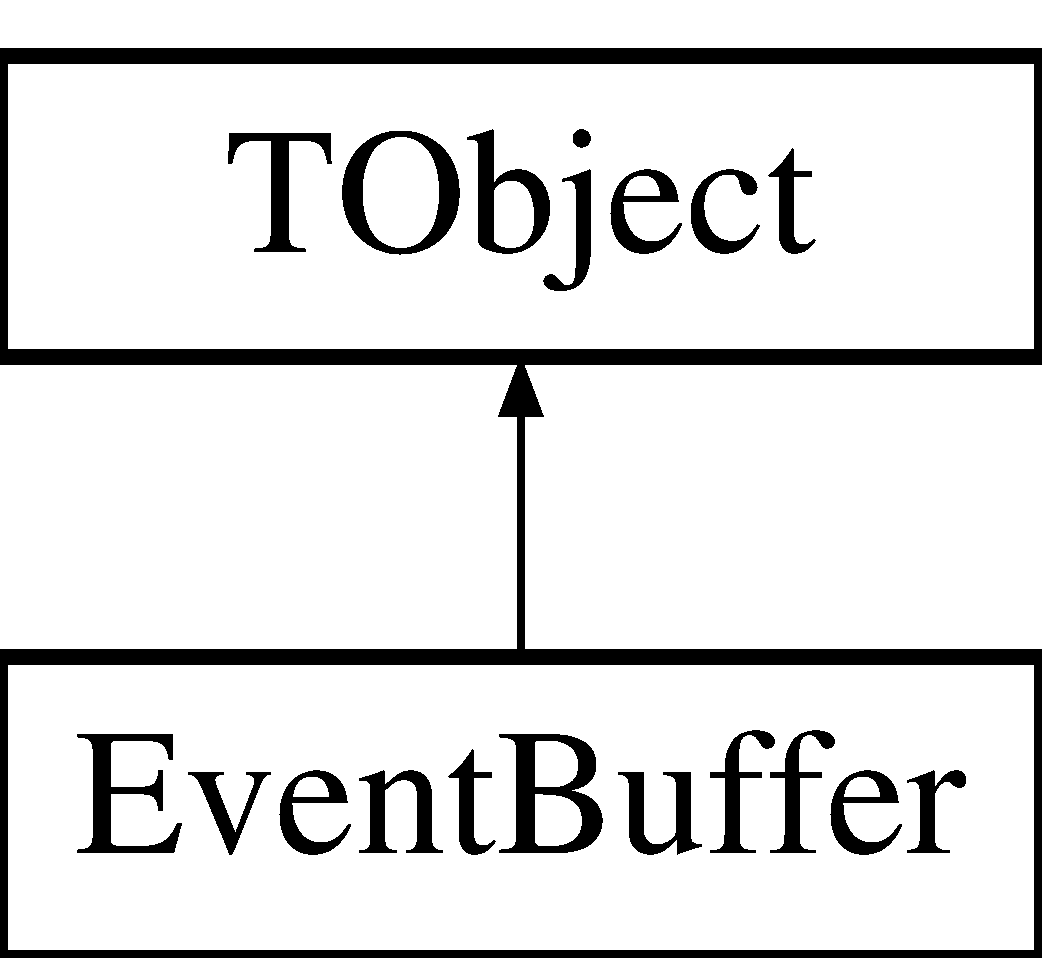
\includegraphics[height=2.000000cm]{class_event_buffer}
\end{center}
\end{figure}
\subsection*{Public Member Functions}
\begin{DoxyCompactItemize}
\item 
\mbox{\Hypertarget{class_event_buffer_a88ffe92cf134a8cd11d3f52ef7533005}\label{class_event_buffer_a88ffe92cf134a8cd11d3f52ef7533005}} 
{\bfseries Event\+Buffer} (\hyperlink{class_global_settings}{Global\+Settings} $\ast$)
\item 
\mbox{\Hypertarget{class_event_buffer_a3517c46566afc4abe5bf635cb84ac685}\label{class_event_buffer_a3517c46566afc4abe5bf635cb84ac685}} 
void {\bfseries Clear\+Evt} ()
\item 
\mbox{\Hypertarget{class_event_buffer_ada9809ccfcc0bb691736cf6f54e270e2}\label{class_event_buffer_ada9809ccfcc0bb691736cf6f54e270e2}} 
void {\bfseries Sort} ()
\item 
\mbox{\Hypertarget{class_event_buffer_af87a5d899fa6f8dd65216eab060febd6}\label{class_event_buffer_af87a5d899fa6f8dd65216eab060febd6}} 
void {\bfseries Event\+Number} (long long event\+Number)
\item 
\mbox{\Hypertarget{class_event_buffer_af109a5cce70d162db4dabd4c0b2c80eb}\label{class_event_buffer_af109a5cce70d162db4dabd4c0b2c80eb}} 
size\+\_\+t {\bfseries Add\+Particle} (unsigned short, \hyperlink{class_adc_sub_event}{Adc\+Sub\+Event} $\ast$, long long, bool, bool, bool)
\item 
\mbox{\Hypertarget{class_event_buffer_a8e6f4c031cd9901aec6d547a3ade0ed4}\label{class_event_buffer_a8e6f4c031cd9901aec6d547a3ade0ed4}} 
size\+\_\+t {\bfseries Add\+Particle} (unsigned short, \hyperlink{class_adc_sub_event}{Adc\+Sub\+Event} $\ast$, bool, bool, bool)
\item 
\mbox{\Hypertarget{class_event_buffer_a66c0da96e0073a20aa5e579ed2336eb7}\label{class_event_buffer_a66c0da96e0073a20aa5e579ed2336eb7}} 
size\+\_\+t {\bfseries Add\+Gamma} (unsigned short, \hyperlink{class_dgf_sub_event}{Dgf\+Sub\+Event} $\ast$)
\item 
\mbox{\Hypertarget{class_event_buffer_aacc0229711693e6df7aa944456c2178f}\label{class_event_buffer_aacc0229711693e6df7aa944456c2178f}} 
void {\bfseries Add\+Timing} (long long, long long, long long)
\item 
\mbox{\Hypertarget{class_event_buffer_a2a1210455f715b292c0424f770ab4703}\label{class_event_buffer_a2a1210455f715b292c0424f770ab4703}} 
size\+\_\+t {\bfseries Number\+Of\+Built\+Events} ()
\item 
\mbox{\Hypertarget{class_event_buffer_afc435d3702c062b229432300057b4c27}\label{class_event_buffer_afc435d3702c062b229432300057b4c27}} 
\hyperlink{class_built_event}{Built\+Event} $\ast$ {\bfseries Get\+Sorted\+Event} (size\+\_\+t)
\end{DoxyCompactItemize}
\subsection*{Protected Attributes}
\begin{DoxyCompactItemize}
\item 
\mbox{\Hypertarget{class_event_buffer_a0c7ee1b008d8ff909977d6c38c010923}\label{class_event_buffer_a0c7ee1b008d8ff909977d6c38c010923}} 
\hyperlink{class_global_settings}{Global\+Settings} $\ast$ {\bfseries Settings}
\item 
\mbox{\Hypertarget{class_event_buffer_ad495f17af4b84135789a21ed0109a239}\label{class_event_buffer_ad495f17af4b84135789a21ed0109a239}} 
bool {\bfseries Sorted}
\item 
\mbox{\Hypertarget{class_event_buffer_a0427cf345d5e88932b754966c21535e1}\label{class_event_buffer_a0427cf345d5e88932b754966c21535e1}} 
unsigned short $\ast$ {\bfseries Sub\+Event\+Number}
\item 
\mbox{\Hypertarget{class_event_buffer_a18101f4a449fbf92fa3c946b0924fb10}\label{class_event_buffer_a18101f4a449fbf92fa3c946b0924fb10}} 
vector$<$ \hyperlink{class_built_event}{Built\+Event} $>$ \hyperlink{class_event_buffer_a18101f4a449fbf92fa3c946b0924fb10}{Built\+Events}
\begin{DoxyCompactList}\small\item\em Built\+Events.\+size() \end{DoxyCompactList}\end{DoxyCompactItemize}


The documentation for this class was generated from the following files\+:\begin{DoxyCompactItemize}
\item 
Med\+To\+Root/Event\+Buffer.\+hh\item 
Med\+To\+Root/Event\+Buffer.\+cc\end{DoxyCompactItemize}

\hypertarget{class_event_builder}{}\section{Event\+Builder Class Reference}
\label{class_event_builder}\index{Event\+Builder@{Event\+Builder}}
Inheritance diagram for Event\+Builder\+:\begin{figure}[H]
\begin{center}
\leavevmode
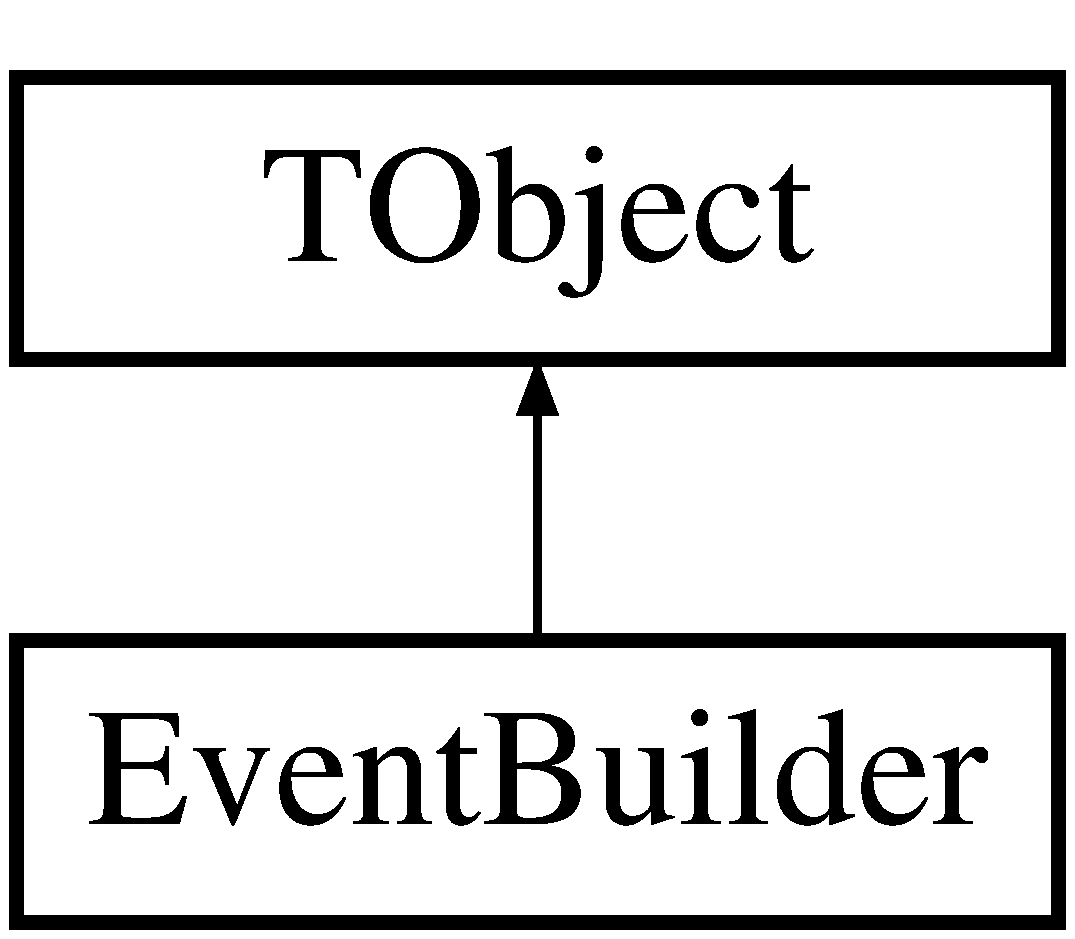
\includegraphics[height=2.000000cm]{class_event_builder}
\end{center}
\end{figure}
\subsection*{Public Member Functions}
\begin{DoxyCompactItemize}
\item 
\mbox{\Hypertarget{class_event_builder_ae5bc6281c66e115f92ab1aad525cc71b}\label{class_event_builder_ae5bc6281c66e115f92ab1aad525cc71b}} 
{\bfseries Event\+Builder} (\hyperlink{class_global_settings}{Global\+Settings} $\ast$)
\item 
\mbox{\Hypertarget{class_event_builder_a19d233a535cc211f91f5de56f4c42e9c}\label{class_event_builder_a19d233a535cc211f91f5de56f4c42e9c}} 
int {\bfseries Trash\+Event} ()
\item 
\mbox{\Hypertarget{class_event_builder_a4e469463e20974bc7be2cfa0ab3874f5}\label{class_event_builder_a4e469463e20974bc7be2cfa0ab3874f5}} 
int {\bfseries Process\+Event} (const M\+B\+S\+Data\+IO $\ast$mbs)
\item 
\mbox{\Hypertarget{class_event_builder_a5e3732d9c2aa0539c0e01e22ce7f5c88}\label{class_event_builder_a5e3732d9c2aa0539c0e01e22ce7f5c88}} 
void {\bfseries Build\+Event} ()
\item 
\mbox{\Hypertarget{class_event_builder_abcc24c43c7bcca0c9e445141349fd816}\label{class_event_builder_abcc24c43c7bcca0c9e445141349fd816}} 
void {\bfseries Finish} ()
\item 
\mbox{\Hypertarget{class_event_builder_a840f7a4c8d9bb81e92007cfb19637bff}\label{class_event_builder_a840f7a4c8d9bb81e92007cfb19637bff}} 
void {\bfseries Statistics} ()
\end{DoxyCompactItemize}


The documentation for this class was generated from the following files\+:\begin{DoxyCompactItemize}
\item 
Med\+To\+Root/Event\+Builder.\+hh\item 
Med\+To\+Root/Event\+Builder.\+cc\end{DoxyCompactItemize}

\hypertarget{classg__clx}{\section{g\-\_\-clx Class Reference}
\label{classg__clx}\index{g\-\_\-clx@{g\-\_\-clx}}
}


Main class for gamma-\/particle coinidence analysis.  




{\ttfamily \#include $<$g\-\_\-clx.\-hh$>$}

Inheritance diagram for g\-\_\-clx\-:\begin{figure}[H]
\begin{center}
\leavevmode
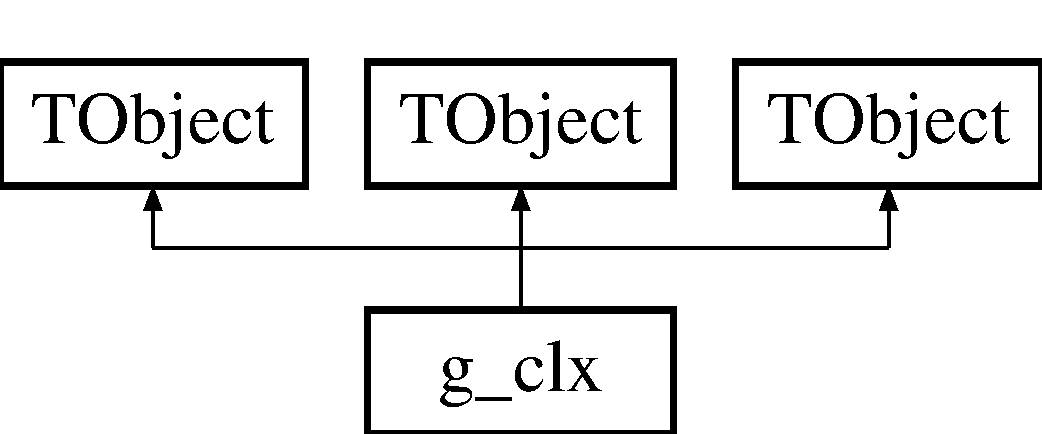
\includegraphics[height=2.000000cm]{classg__clx}
\end{center}
\end{figure}
\subsection*{Public Member Functions}
\begin{DoxyCompactItemize}
\item 
\hypertarget{classg__clx_aa619daf508fe1d6bddb000af26630f31}{\hyperlink{classg__clx_aa619daf508fe1d6bddb000af26630f31}{g\-\_\-clx} (T\-Tree $\ast$tree=0)}\label{classg__clx_aa619daf508fe1d6bddb000af26630f31}

\begin{DoxyCompactList}\small\item\em Constructor\-: if parameter tree is not specified (or zero), probably crash. \end{DoxyCompactList}\item 
\hypertarget{classg__clx_adbe899d82aba9fc16ec17f47c0ce894e}{virtual \hyperlink{classg__clx_adbe899d82aba9fc16ec17f47c0ce894e}{$\sim$g\-\_\-clx} ()}\label{classg__clx_adbe899d82aba9fc16ec17f47c0ce894e}

\begin{DoxyCompactList}\small\item\em Destructor. \end{DoxyCompactList}\item 
\hypertarget{classg__clx_ab4c53e12e70c3671ff8895fc388dd7d2}{virtual Int\-\_\-t \hyperlink{classg__clx_ab4c53e12e70c3671ff8895fc388dd7d2}{Get\-Entry} (Long64\-\_\-t entry)}\label{classg__clx_ab4c53e12e70c3671ff8895fc388dd7d2}

\begin{DoxyCompactList}\small\item\em Read contents of entry. \end{DoxyCompactList}\item 
\hypertarget{classg__clx_a0aab3745bdb3db08757c974eebffbe39}{virtual Long64\-\_\-t \hyperlink{classg__clx_a0aab3745bdb3db08757c974eebffbe39}{Load\-Tree} (Long64\-\_\-t entry)}\label{classg__clx_a0aab3745bdb3db08757c974eebffbe39}

\begin{DoxyCompactList}\small\item\em Set the environment to read one entry. \end{DoxyCompactList}\item 
virtual void \hyperlink{classg__clx_a92531261155ea15bee6b74c7e491132a}{Init} (T\-Tree $\ast$tree)
\item 
virtual void \hyperlink{classg__clx_a9d5de859df4bfbb746726661ff1d24a9}{Loop} (string outputfilename)
\item 
virtual Bool\-\_\-t \hyperlink{classg__clx_a1fe81316168bc18dc2325ca5595577a9}{Notify} ()
\item 
virtual void \hyperlink{classg__clx_ae86183470c7bb8db45753aa4c86f1d41}{Show} (Long64\-\_\-t entry=-\/1)
\item 
\hypertarget{classg__clx_a8d0a8ed3a7cc55ca97aeb77f4183d3b8}{{\bfseries Class\-Def} (\hyperlink{classg__clx}{g\-\_\-clx}, 1)}\label{classg__clx_a8d0a8ed3a7cc55ca97aeb77f4183d3b8}

\end{DoxyCompactItemize}
\subsection*{Public Attributes}
\begin{DoxyCompactItemize}
\item 
\hypertarget{classg__clx_aa0c1129a726bb6a3bda4197decf634f2}{T\-Tree $\ast$ {\bfseries f\-Chain}}\label{classg__clx_aa0c1129a726bb6a3bda4197decf634f2}

\item 
\hypertarget{classg__clx_a4ebe765901e5abf5d740a59edd2796d3}{Int\-\_\-t \hyperlink{classg__clx_a4ebe765901e5abf5d740a59edd2796d3}{f\-Current}}\label{classg__clx_a4ebe765901e5abf5d740a59edd2796d3}

\begin{DoxyCompactList}\small\item\em pointer to the analyzed T\-Tree or T\-Chain \end{DoxyCompactList}\item 
\hypertarget{classg__clx_abf3f260c2d2f9884a9f6b041f54ec94a}{U\-Int\-\_\-t \hyperlink{classg__clx_abf3f260c2d2f9884a9f6b041f54ec94a}{f\-Unique\-I\-D}}\label{classg__clx_abf3f260c2d2f9884a9f6b041f54ec94a}

\begin{DoxyCompactList}\small\item\em current Tree number in a T\-Chain \end{DoxyCompactList}\item 
\hypertarget{classg__clx_a7206bd09efca58552eea94544746280e}{U\-Int\-\_\-t {\bfseries f\-Bits}}\label{classg__clx_a7206bd09efca58552eea94544746280e}

\item 
\hypertarget{classg__clx_afa1d8a83322f5f91c433b1747ffdc71b}{float \hyperlink{classg__clx_afa1d8a83322f5f91c433b1747ffdc71b}{gen}}\label{classg__clx_afa1d8a83322f5f91c433b1747ffdc71b}

\begin{DoxyCompactList}\small\item\em gamma-\/ray energy in ke\-V \end{DoxyCompactList}\item 
\hypertarget{classg__clx_a0cc2a584a4f5152751778ee68bcdb743}{int \hyperlink{classg__clx_a0cc2a584a4f5152751778ee68bcdb743}{cid}}\label{classg__clx_a0cc2a584a4f5152751778ee68bcdb743}

\begin{DoxyCompactList}\small\item\em core I\-D from 0 to 23 \end{DoxyCompactList}\item 
\hypertarget{classg__clx_a04f33012ec56804fca6978885732bc8f}{int \hyperlink{classg__clx_a04f33012ec56804fca6978885732bc8f}{sid}}\label{classg__clx_a04f33012ec56804fca6978885732bc8f}

\begin{DoxyCompactList}\small\item\em segment I\-D from 0 to 6 (zero is the core) \end{DoxyCompactList}\item 
\hypertarget{classg__clx_af057b9309517174aa3f45d0357b594e0}{int \hyperlink{classg__clx_af057b9309517174aa3f45d0357b594e0}{cluid}}\label{classg__clx_af057b9309517174aa3f45d0357b594e0}

\begin{DoxyCompactList}\small\item\em cluster I\-D from 0 to 7 \end{DoxyCompactList}\item 
\hypertarget{classg__clx_a1add23d784b2694a2f680b855480d95f}{float \hyperlink{classg__clx_a1add23d784b2694a2f680b855480d95f}{tha}}\label{classg__clx_a1add23d784b2694a2f680b855480d95f}

\begin{DoxyCompactList}\small\item\em gamma-\/ray theta angle in radians (not yet implemented) \end{DoxyCompactList}\item 
\hypertarget{classg__clx_affd7b8c1191e11bab79d77dfb4f16a63}{float \hyperlink{classg__clx_affd7b8c1191e11bab79d77dfb4f16a63}{pha}}\label{classg__clx_affd7b8c1191e11bab79d77dfb4f16a63}

\begin{DoxyCompactList}\small\item\em gamm-\/ray phi angle in radians (not yet implemented) \end{DoxyCompactList}\item 
\hypertarget{classg__clx_ae3b41efe9dfca0e33b8bba9e737ee421}{vector$<$ float $>$ \hyperlink{classg__clx_ae3b41efe9dfca0e33b8bba9e737ee421}{gcor\-\_\-gen}}\label{classg__clx_ae3b41efe9dfca0e33b8bba9e737ee421}

\begin{DoxyCompactList}\small\item\em vector of correlated gamma-\/ray energies in ke\-V \end{DoxyCompactList}\item 
\hypertarget{classg__clx_a0aed9e2ec9d94795c86a00c51d940652}{vector$<$ int $>$ \hyperlink{classg__clx_a0aed9e2ec9d94795c86a00c51d940652}{gcor\-\_\-cid}}\label{classg__clx_a0aed9e2ec9d94795c86a00c51d940652}

\begin{DoxyCompactList}\small\item\em vector of correlated core I\-Ds \end{DoxyCompactList}\item 
\hypertarget{classg__clx_a10ddb8a6039959138b145dec9979a216}{vector$<$ int $>$ \hyperlink{classg__clx_a10ddb8a6039959138b145dec9979a216}{gcor\-\_\-sid}}\label{classg__clx_a10ddb8a6039959138b145dec9979a216}

\begin{DoxyCompactList}\small\item\em vector of correlated segment I\-Ds \end{DoxyCompactList}\item 
\hypertarget{classg__clx_a93666f6d2ee0818e554d9188df02b844}{vector$<$ int $>$ \hyperlink{classg__clx_a93666f6d2ee0818e554d9188df02b844}{gcor\-\_\-cluid}}\label{classg__clx_a93666f6d2ee0818e554d9188df02b844}

\begin{DoxyCompactList}\small\item\em vector of correlated cluster I\-Ds \end{DoxyCompactList}\item 
\hypertarget{classg__clx_a19c4bfa4d9f2d4ef26399075bba0c2d2}{vector$<$ float $>$ \hyperlink{classg__clx_a19c4bfa4d9f2d4ef26399075bba0c2d2}{gcor\-\_\-tha}}\label{classg__clx_a19c4bfa4d9f2d4ef26399075bba0c2d2}

\begin{DoxyCompactList}\small\item\em vector of correlated theta angles \end{DoxyCompactList}\item 
\hypertarget{classg__clx_a823ddd84f64de88789bfa434579778dc}{vector$<$ float $>$ \hyperlink{classg__clx_a823ddd84f64de88789bfa434579778dc}{gcor\-\_\-pha}}\label{classg__clx_a823ddd84f64de88789bfa434579778dc}

\begin{DoxyCompactList}\small\item\em vector of correlated phi angles \end{DoxyCompactList}\item 
\hypertarget{classg__clx_a7a01f0832f4e7f7737179ddcc7b74b7b}{vector$<$ float $>$ \hyperlink{classg__clx_a7a01f0832f4e7f7737179ddcc7b74b7b}{gcor\-\_\-gtd}}\label{classg__clx_a7a01f0832f4e7f7737179ddcc7b74b7b}

\begin{DoxyCompactList}\small\item\em vector of time-\/difference to original gamma-\/ray \end{DoxyCompactList}\item 
\hypertarget{classg__clx_a69177d2d636c68b6e20b26b3166421a0}{vector$<$ float $>$ \hyperlink{classg__clx_a69177d2d636c68b6e20b26b3166421a0}{pen}}\label{classg__clx_a69177d2d636c68b6e20b26b3166421a0}

\begin{DoxyCompactList}\small\item\em particle energies \end{DoxyCompactList}\item 
\hypertarget{classg__clx_ad1cc659d52f0fc7616fff4d94c9ca6ea}{vector$<$ double $>$ \hyperlink{classg__clx_ad1cc659d52f0fc7616fff4d94c9ca6ea}{time}}\label{classg__clx_ad1cc659d52f0fc7616fff4d94c9ca6ea}

\begin{DoxyCompactList}\small\item\em particle timestamps \end{DoxyCompactList}\item 
\hypertarget{classg__clx_a98fc719d6f94e8f1ccecb4978972699d}{vector$<$ double $>$ \hyperlink{classg__clx_a98fc719d6f94e8f1ccecb4978972699d}{sst}}\label{classg__clx_a98fc719d6f94e8f1ccecb4978972699d}

\begin{DoxyCompactList}\small\item\em supercycle timestamps \end{DoxyCompactList}\item 
\hypertarget{classg__clx_a2adb67934c7e26d01a5faa8ccb6c9c15}{vector$<$ float $>$ \hyperlink{classg__clx_a2adb67934c7e26d01a5faa8ccb6c9c15}{td}}\label{classg__clx_a2adb67934c7e26d01a5faa8ccb6c9c15}

\begin{DoxyCompactList}\small\item\em particle-\/gamma time difference in 25 ns timestamps \end{DoxyCompactList}\item 
\hypertarget{classg__clx_ad017e828f9374d881ad4eac9e6ea1818}{vector$<$ int $>$ \hyperlink{classg__clx_ad017e828f9374d881ad4eac9e6ea1818}{ann}}\label{classg__clx_ad017e828f9374d881ad4eac9e6ea1818}

\begin{DoxyCompactList}\small\item\em annular (front) strip I\-D of particle (0 = outer; 15 inner) \end{DoxyCompactList}\item 
\hypertarget{classg__clx_a556dd0017434edf15b8ec9e25437a932}{vector$<$ int $>$ \hyperlink{classg__clx_a556dd0017434edf15b8ec9e25437a932}{sec}}\label{classg__clx_a556dd0017434edf15b8ec9e25437a932}

\begin{DoxyCompactList}\small\item\em secular (back) strip I\-D of particle (0 to 12; clockwise wrt beam) \end{DoxyCompactList}\item 
\hypertarget{classg__clx_af736c71de60d093f141cae033d675387}{vector$<$ int $>$ \hyperlink{classg__clx_af736c71de60d093f141cae033d675387}{det}}\label{classg__clx_af736c71de60d093f141cae033d675387}

\begin{DoxyCompactList}\small\item\em detector (quadrant) number of particle \end{DoxyCompactList}\item 
\hypertarget{classg__clx_a8bab7b24f203a20b19f1cbb565d176ad}{vector$<$ int $>$ \hyperlink{classg__clx_a8bab7b24f203a20b19f1cbb565d176ad}{coin}}\label{classg__clx_a8bab7b24f203a20b19f1cbb565d176ad}

\begin{DoxyCompactList}\small\item\em coincidence flag\-: 0 = prompt, 1 = random, 2 = delayed, -\/1 = none \end{DoxyCompactList}\item 
\hypertarget{classg__clx_a636dfc5c0302782a3a021dff3f6ec53e}{int \hyperlink{classg__clx_a636dfc5c0302782a3a021dff3f6ec53e}{laser}}\label{classg__clx_a636dfc5c0302782a3a021dff3f6ec53e}

\begin{DoxyCompactList}\small\item\em laser on/off flag\-: 1 = on, 0 = off \end{DoxyCompactList}\item 
\hypertarget{classg__clx_ab238ce0805d4af78ff43b999360a28f4}{int \hyperlink{classg__clx_ab238ce0805d4af78ff43b999360a28f4}{pr\-\_\-hits}}\label{classg__clx_ab238ce0805d4af78ff43b999360a28f4}

\begin{DoxyCompactList}\small\item\em number of prompt hits \end{DoxyCompactList}\item 
\hypertarget{classg__clx_a2ca61cc109e9e0580f35a4baa5ca4b21}{int \hyperlink{classg__clx_a2ca61cc109e9e0580f35a4baa5ca4b21}{rndm\-\_\-hits}}\label{classg__clx_a2ca61cc109e9e0580f35a4baa5ca4b21}

\begin{DoxyCompactList}\small\item\em number of random hits \end{DoxyCompactList}\item 
\hypertarget{classg__clx_a1205d577537a7131563e281be99f4a97}{int \hyperlink{classg__clx_a1205d577537a7131563e281be99f4a97}{del\-\_\-hits}}\label{classg__clx_a1205d577537a7131563e281be99f4a97}

\begin{DoxyCompactList}\small\item\em number of delayed hits \end{DoxyCompactList}\item 
\hypertarget{classg__clx_a33325f12a127d94cc10a8cc491df2f15}{vector$<$ int $>$ \hyperlink{classg__clx_a33325f12a127d94cc10a8cc491df2f15}{pr\-\_\-ptr}}\label{classg__clx_a33325f12a127d94cc10a8cc491df2f15}

\begin{DoxyCompactList}\small\item\em pointer to prompt hits in particle vector/array \end{DoxyCompactList}\item 
\hypertarget{classg__clx_a5dee420c080c876ed2c5467ec212d3f7}{vector$<$ int $>$ \hyperlink{classg__clx_a5dee420c080c876ed2c5467ec212d3f7}{rndm\-\_\-ptr}}\label{classg__clx_a5dee420c080c876ed2c5467ec212d3f7}

\begin{DoxyCompactList}\small\item\em pointer to random hits in particle vector/array \end{DoxyCompactList}\item 
\hypertarget{classg__clx_a8514273470549549d94417e7cade9b82}{vector$<$ int $>$ \hyperlink{classg__clx_a8514273470549549d94417e7cade9b82}{del\-\_\-ptr}}\label{classg__clx_a8514273470549549d94417e7cade9b82}

\begin{DoxyCompactList}\small\item\em pointer to delayed hits in particle vector/array \end{DoxyCompactList}\item 
\hypertarget{classg__clx_a4b7f5bc375e032d31bebb6ba34cb328f}{int {\bfseries file}}\label{classg__clx_a4b7f5bc375e032d31bebb6ba34cb328f}

\item 
\hypertarget{classg__clx_aade220d336f2c91d09b4da5a14138436}{float {\bfseries Gamma\-Energy}}\label{classg__clx_aade220d336f2c91d09b4da5a14138436}

\item 
\hypertarget{classg__clx_a10f3a51541a437abeafdde5e4d919296}{int {\bfseries Zb}}\label{classg__clx_a10f3a51541a437abeafdde5e4d919296}

\item 
\hypertarget{classg__clx_af3a63ef9a4e0e92e6646ec8c9e86cd2d}{int {\bfseries Zt}}\label{classg__clx_af3a63ef9a4e0e92e6646ec8c9e86cd2d}

\item 
\hypertarget{classg__clx_a9806f6d9aa4ecd6daeccd1f8184bbb5e}{float {\bfseries Ab}}\label{classg__clx_a9806f6d9aa4ecd6daeccd1f8184bbb5e}

\item 
\hypertarget{classg__clx_a0a85cb0adca7a54ed29ebda550b36dcc}{float {\bfseries At}}\label{classg__clx_a0a85cb0adca7a54ed29ebda550b36dcc}

\item 
\hypertarget{classg__clx_adacfaa00cabbde7095f23a1cacab7510}{float {\bfseries Eb}}\label{classg__clx_adacfaa00cabbde7095f23a1cacab7510}

\item 
\hypertarget{classg__clx_a1f2096a705a986c48af8540f6eb1b835}{float {\bfseries Ex}}\label{classg__clx_a1f2096a705a986c48af8540f6eb1b835}

\item 
\hypertarget{classg__clx_ada5b4790b6f1970cd350444564604e2f}{float {\bfseries thick}}\label{classg__clx_ada5b4790b6f1970cd350444564604e2f}

\item 
\hypertarget{classg__clx_a55b2ad47323975fbefd70314a1580d26}{float {\bfseries depth}}\label{classg__clx_a55b2ad47323975fbefd70314a1580d26}

\item 
\hypertarget{classg__clx_a85780ae170aef9d5362a47520ee3a822}{float \hyperlink{classg__clx_a85780ae170aef9d5362a47520ee3a822}{zoffset}}\label{classg__clx_a85780ae170aef9d5362a47520ee3a822}

\begin{DoxyCompactList}\small\item\em offset of the target with respect to the origin in mm (beam direction positive) \end{DoxyCompactList}\item 
\hypertarget{classg__clx_af6483d6ed4f21d91fe1ac7e88393ab4e}{float \hyperlink{classg__clx_af6483d6ed4f21d91fe1ac7e88393ab4e}{cddist}}\label{classg__clx_af6483d6ed4f21d91fe1ac7e88393ab4e}

\begin{DoxyCompactList}\small\item\em relative distance between the C\-D and target in mm \end{DoxyCompactList}\item 
\hypertarget{classg__clx_a2f16d48f2601cfd6ccb100283f3cdab7}{float \hyperlink{classg__clx_a2f16d48f2601cfd6ccb100283f3cdab7}{cdoffset}}\label{classg__clx_a2f16d48f2601cfd6ccb100283f3cdab7}

\begin{DoxyCompactList}\small\item\em phi rotation of C\-D wrt to (det=0;sec=0) at vertical \end{DoxyCompactList}\item 
\hypertarget{classg__clx_a9868b722188e951233b134083dd63370}{float \hyperlink{classg__clx_a9868b722188e951233b134083dd63370}{deadlayer}}\label{classg__clx_a9868b722188e951233b134083dd63370}

\begin{DoxyCompactList}\small\item\em deadlayer thickness in mm \end{DoxyCompactList}\item 
\hypertarget{classg__clx_a9093a10412ab047b3b910e4c4a9d70d1}{float \hyperlink{classg__clx_a9093a10412ab047b3b910e4c4a9d70d1}{contaminant}}\label{classg__clx_a9093a10412ab047b3b910e4c4a9d70d1}

\begin{DoxyCompactList}\small\item\em contaminant layer thickness in mg/cm$^\wedge$2 \end{DoxyCompactList}\item 
\hypertarget{classg__clx_aca4cd80422665dab4188cbf82bb569ce}{float \hyperlink{classg__clx_aca4cd80422665dab4188cbf82bb569ce}{spededist}}\label{classg__clx_aca4cd80422665dab4188cbf82bb569ce}

\begin{DoxyCompactList}\small\item\em S\-P\-E\-D\-E to target distance in mm. \end{DoxyCompactList}\item 
\hypertarget{classg__clx_ad9d34b2f15cdb59de8b46f1f68280c5c}{float \hyperlink{classg__clx_ad9d34b2f15cdb59de8b46f1f68280c5c}{bg\-\_\-frac}}\label{classg__clx_ad9d34b2f15cdb59de8b46f1f68280c5c}

\begin{DoxyCompactList}\small\item\em ratio of prompt and random background subtraction (negative) \end{DoxyCompactList}\item 
\hypertarget{classg__clx_a626bb40b10360e2572d0c489a0cde2ad}{T\-Cut\-G $\ast$ \hyperlink{classg__clx_a626bb40b10360e2572d0c489a0cde2ad}{Bcut}}\label{classg__clx_a626bb40b10360e2572d0c489a0cde2ad}

\begin{DoxyCompactList}\small\item\em Graphical cut for beam-\/like particles. \end{DoxyCompactList}\item 
\hypertarget{classg__clx_a5607f06b4881cc2843fd2b9c9c16b35b}{T\-Cut\-G $\ast$ \hyperlink{classg__clx_a5607f06b4881cc2843fd2b9c9c16b35b}{Tcut}}\label{classg__clx_a5607f06b4881cc2843fd2b9c9c16b35b}

\begin{DoxyCompactList}\small\item\em Graphical cut for target-\/like particles. \end{DoxyCompactList}\item 
\hypertarget{classg__clx_ada0e05bae03e42e14c8e8494122a1709}{T\-Branch $\ast$ {\bfseries b\-\_\-mbevts\-\_\-f\-Unique\-I\-D}}\label{classg__clx_ada0e05bae03e42e14c8e8494122a1709}

\item 
\hypertarget{classg__clx_ad19ba31973ff37f5351edf88f4dbf5aa}{T\-Branch $\ast$ {\bfseries b\-\_\-mbevts\-\_\-f\-Bits}}\label{classg__clx_ad19ba31973ff37f5351edf88f4dbf5aa}

\item 
\hypertarget{classg__clx_abfc7aed653b54224fb7ae61efd081de6}{T\-Branch $\ast$ {\bfseries b\-\_\-mbevts\-\_\-gen}}\label{classg__clx_abfc7aed653b54224fb7ae61efd081de6}

\item 
\hypertarget{classg__clx_a4b7eebd7443d5a9058d4c21aca44e6bc}{T\-Branch $\ast$ {\bfseries b\-\_\-mbevts\-\_\-cid}}\label{classg__clx_a4b7eebd7443d5a9058d4c21aca44e6bc}

\item 
\hypertarget{classg__clx_a80f356c60fe1eea5e82fcba16b4d482b}{T\-Branch $\ast$ {\bfseries b\-\_\-mbevts\-\_\-sid}}\label{classg__clx_a80f356c60fe1eea5e82fcba16b4d482b}

\item 
\hypertarget{classg__clx_ae91752a1092e7b3ec6191515378fbd63}{T\-Branch $\ast$ {\bfseries b\-\_\-mbevts\-\_\-cluid}}\label{classg__clx_ae91752a1092e7b3ec6191515378fbd63}

\item 
\hypertarget{classg__clx_a7c4dd347f0cf1856c3aaca6c77a3280a}{T\-Branch $\ast$ {\bfseries b\-\_\-mbevts\-\_\-tha}}\label{classg__clx_a7c4dd347f0cf1856c3aaca6c77a3280a}

\item 
\hypertarget{classg__clx_ae9e6b4ef1483c136f08a0bd34ff3c98a}{T\-Branch $\ast$ {\bfseries b\-\_\-mbevts\-\_\-pha}}\label{classg__clx_ae9e6b4ef1483c136f08a0bd34ff3c98a}

\item 
\hypertarget{classg__clx_a272e88232977ef4a5537d35dea2abb53}{T\-Branch $\ast$ {\bfseries b\-\_\-mbevts\-\_\-gcor\-\_\-gen}}\label{classg__clx_a272e88232977ef4a5537d35dea2abb53}

\item 
\hypertarget{classg__clx_a3fd25e2237b246bfea4505b3df5f18f6}{T\-Branch $\ast$ {\bfseries b\-\_\-mbevts\-\_\-gcor\-\_\-cid}}\label{classg__clx_a3fd25e2237b246bfea4505b3df5f18f6}

\item 
\hypertarget{classg__clx_ade7b131c7bdc5550ee4f7564a562ebbf}{T\-Branch $\ast$ {\bfseries b\-\_\-mbevts\-\_\-gcor\-\_\-sid}}\label{classg__clx_ade7b131c7bdc5550ee4f7564a562ebbf}

\item 
\hypertarget{classg__clx_ae23d5724733086d7e63dc3f69a5785ae}{T\-Branch $\ast$ {\bfseries b\-\_\-mbevts\-\_\-gcor\-\_\-cluid}}\label{classg__clx_ae23d5724733086d7e63dc3f69a5785ae}

\item 
\hypertarget{classg__clx_a014cf5b11b0198747192d29bbf506066}{T\-Branch $\ast$ {\bfseries b\-\_\-mbevts\-\_\-gcor\-\_\-tha}}\label{classg__clx_a014cf5b11b0198747192d29bbf506066}

\item 
\hypertarget{classg__clx_aba6a6fa2f721ae370bac54aae22c793e}{T\-Branch $\ast$ {\bfseries b\-\_\-mbevts\-\_\-gcor\-\_\-pha}}\label{classg__clx_aba6a6fa2f721ae370bac54aae22c793e}

\item 
\hypertarget{classg__clx_af3eb18cba48802757fe342cd7f04d15b}{T\-Branch $\ast$ {\bfseries b\-\_\-mbevts\-\_\-gcor\-\_\-gtd}}\label{classg__clx_af3eb18cba48802757fe342cd7f04d15b}

\item 
\hypertarget{classg__clx_a798da42e3e08624f65e7a62e72768731}{T\-Branch $\ast$ {\bfseries b\-\_\-mbevts\-\_\-pen}}\label{classg__clx_a798da42e3e08624f65e7a62e72768731}

\item 
\hypertarget{classg__clx_a4d33de820956789eb93800fdc7ac810d}{T\-Branch $\ast$ {\bfseries b\-\_\-mbevts\-\_\-time}}\label{classg__clx_a4d33de820956789eb93800fdc7ac810d}

\item 
\hypertarget{classg__clx_a336653d8862dabf46279816252cd9a67}{T\-Branch $\ast$ {\bfseries b\-\_\-mbevts\-\_\-sst}}\label{classg__clx_a336653d8862dabf46279816252cd9a67}

\item 
\hypertarget{classg__clx_a11241953b3c0bfb60e12b5e958c33000}{T\-Branch $\ast$ {\bfseries b\-\_\-mbevts\-\_\-td}}\label{classg__clx_a11241953b3c0bfb60e12b5e958c33000}

\item 
\hypertarget{classg__clx_a68936e16782c4be67cd3c4ce8eae7132}{T\-Branch $\ast$ {\bfseries b\-\_\-mbevts\-\_\-ann}}\label{classg__clx_a68936e16782c4be67cd3c4ce8eae7132}

\item 
\hypertarget{classg__clx_a8a0b2b747bcfca112170739a6bd7d51e}{T\-Branch $\ast$ {\bfseries b\-\_\-mbevts\-\_\-sec}}\label{classg__clx_a8a0b2b747bcfca112170739a6bd7d51e}

\item 
\hypertarget{classg__clx_a73c68a34850432a3402d572e91973f98}{T\-Branch $\ast$ {\bfseries b\-\_\-mbevts\-\_\-det}}\label{classg__clx_a73c68a34850432a3402d572e91973f98}

\item 
\hypertarget{classg__clx_aea150013c3823082bf94c6fe7c92c643}{T\-Branch $\ast$ {\bfseries b\-\_\-mbevts\-\_\-coin}}\label{classg__clx_aea150013c3823082bf94c6fe7c92c643}

\item 
\hypertarget{classg__clx_a654f79962aec1454c9e297b89f3a8beb}{T\-Branch $\ast$ {\bfseries b\-\_\-mbevts\-\_\-laser}}\label{classg__clx_a654f79962aec1454c9e297b89f3a8beb}

\item 
\hypertarget{classg__clx_a8604c42bddbbf63ea8cf7f3e1af36cf3}{T\-Branch $\ast$ {\bfseries b\-\_\-mbevts\-\_\-pr\-\_\-hits}}\label{classg__clx_a8604c42bddbbf63ea8cf7f3e1af36cf3}

\item 
\hypertarget{classg__clx_a5a8055b0d581696cd84f6a4b5b4c582f}{T\-Branch $\ast$ {\bfseries b\-\_\-mbevts\-\_\-rndm\-\_\-hits}}\label{classg__clx_a5a8055b0d581696cd84f6a4b5b4c582f}

\item 
\hypertarget{classg__clx_ab7d9842b440289a2274a926e7611bb2c}{T\-Branch $\ast$ {\bfseries b\-\_\-mbevts\-\_\-del\-\_\-hits}}\label{classg__clx_ab7d9842b440289a2274a926e7611bb2c}

\item 
\hypertarget{classg__clx_a9d647b0e87c194c34d426c949f610843}{T\-Branch $\ast$ {\bfseries b\-\_\-mbevts\-\_\-pr\-\_\-ptr}}\label{classg__clx_a9d647b0e87c194c34d426c949f610843}

\item 
\hypertarget{classg__clx_a992d0d4203d4ab5327153a81f199942f}{T\-Branch $\ast$ {\bfseries b\-\_\-mbevts\-\_\-rndm\-\_\-ptr}}\label{classg__clx_a992d0d4203d4ab5327153a81f199942f}

\item 
\hypertarget{classg__clx_a30a5429830731f534a82e57fd7c6c589}{T\-Branch $\ast$ {\bfseries b\-\_\-mbevts\-\_\-del\-\_\-ptr}}\label{classg__clx_a30a5429830731f534a82e57fd7c6c589}

\item 
\hypertarget{classg__clx_a76bc22e5d25b02dd39e4b22369bbcb46}{T\-Branch $\ast$ {\bfseries b\-\_\-mbevts\-\_\-file}}\label{classg__clx_a76bc22e5d25b02dd39e4b22369bbcb46}

\end{DoxyCompactItemize}


\subsection{Detailed Description}
Main class for gamma-\/particle coinidence analysis. 

\subsection{Member Function Documentation}
\hypertarget{classg__clx_a92531261155ea15bee6b74c7e491132a}{\index{g\-\_\-clx@{g\-\_\-clx}!Init@{Init}}
\index{Init@{Init}!g_clx@{g\-\_\-clx}}
\subsubsection[{Init}]{\setlength{\rightskip}{0pt plus 5cm}virtual void g\-\_\-clx\-::\-Init (
\begin{DoxyParamCaption}
\item[{T\-Tree $\ast$}]{tree}
\end{DoxyParamCaption}
)\hspace{0.3cm}{\ttfamily [virtual]}}}\label{classg__clx_a92531261155ea15bee6b74c7e491132a}
The \hyperlink{classg__clx_a92531261155ea15bee6b74c7e491132a}{Init()} function is called when the selector needs to initialize a new tree or chain. Typically here the branch addresses and branch pointers of the tree will be set. It is normally not necessary to make changes to the generated code, but the routine can be extended by the user if needed. \hyperlink{classg__clx_a92531261155ea15bee6b74c7e491132a}{Init()} will be called many times when running on P\-R\-O\-O\-F (once per file to be processed). \hypertarget{classg__clx_a9d5de859df4bfbb746726661ff1d24a9}{\index{g\-\_\-clx@{g\-\_\-clx}!Loop@{Loop}}
\index{Loop@{Loop}!g_clx@{g\-\_\-clx}}
\subsubsection[{Loop}]{\setlength{\rightskip}{0pt plus 5cm}void g\-\_\-clx\-::\-Loop (
\begin{DoxyParamCaption}
\item[{string}]{outputfilename}
\end{DoxyParamCaption}
)\hspace{0.3cm}{\ttfamily [virtual]}}}\label{classg__clx_a9d5de859df4bfbb746726661ff1d24a9}
This is the main logic routine for sorting the data. It shouldn't really be played with, except there are still some harcoded values that don't really make sense anymore. The ones that are useful will be moved to the config file/input and the ones that aren't will be deleted. You will also find the Miniball cluster angles hardcoded here too. They will eventually be moved to the Tree\-Builder stage. \hypertarget{classg__clx_a1fe81316168bc18dc2325ca5595577a9}{\index{g\-\_\-clx@{g\-\_\-clx}!Notify@{Notify}}
\index{Notify@{Notify}!g_clx@{g\-\_\-clx}}
\subsubsection[{Notify}]{\setlength{\rightskip}{0pt plus 5cm}virtual Bool\-\_\-t g\-\_\-clx\-::\-Notify (
\begin{DoxyParamCaption}
{}
\end{DoxyParamCaption}
)\hspace{0.3cm}{\ttfamily [virtual]}}}\label{classg__clx_a1fe81316168bc18dc2325ca5595577a9}
The \hyperlink{classg__clx_a1fe81316168bc18dc2325ca5595577a9}{Notify()} function is called when a new file is opened. This can be either for a new T\-Tree in a T\-Chain or when when a new T\-Tree is started when using P\-R\-O\-O\-F. It is normally not necessary to make changes to the generated code, but the routine can be extended by the user if needed. The return value is currently not used. \hypertarget{classg__clx_ae86183470c7bb8db45753aa4c86f1d41}{\index{g\-\_\-clx@{g\-\_\-clx}!Show@{Show}}
\index{Show@{Show}!g_clx@{g\-\_\-clx}}
\subsubsection[{Show}]{\setlength{\rightskip}{0pt plus 5cm}virtual void g\-\_\-clx\-::\-Show (
\begin{DoxyParamCaption}
\item[{Long64\-\_\-t}]{entry = {\ttfamily -\/1}}
\end{DoxyParamCaption}
)\hspace{0.3cm}{\ttfamily [virtual]}}}\label{classg__clx_ae86183470c7bb8db45753aa4c86f1d41}
Print contents of entry. If entry is not specified, print current entry 

The documentation for this class was generated from the following files\-:\begin{DoxyCompactItemize}
\item 
C\-L\-X\-Ana/g\-\_\-clx.\-hh\item 
C\-L\-X\-Ana/g\-\_\-clx.\-cc\end{DoxyCompactItemize}

\hypertarget{class_global_settings}{\section{Global\-Settings Class Reference}
\label{class_global_settings}\index{Global\-Settings@{Global\-Settings}}
}
Inheritance diagram for Global\-Settings\-:\begin{figure}[H]
\begin{center}
\leavevmode
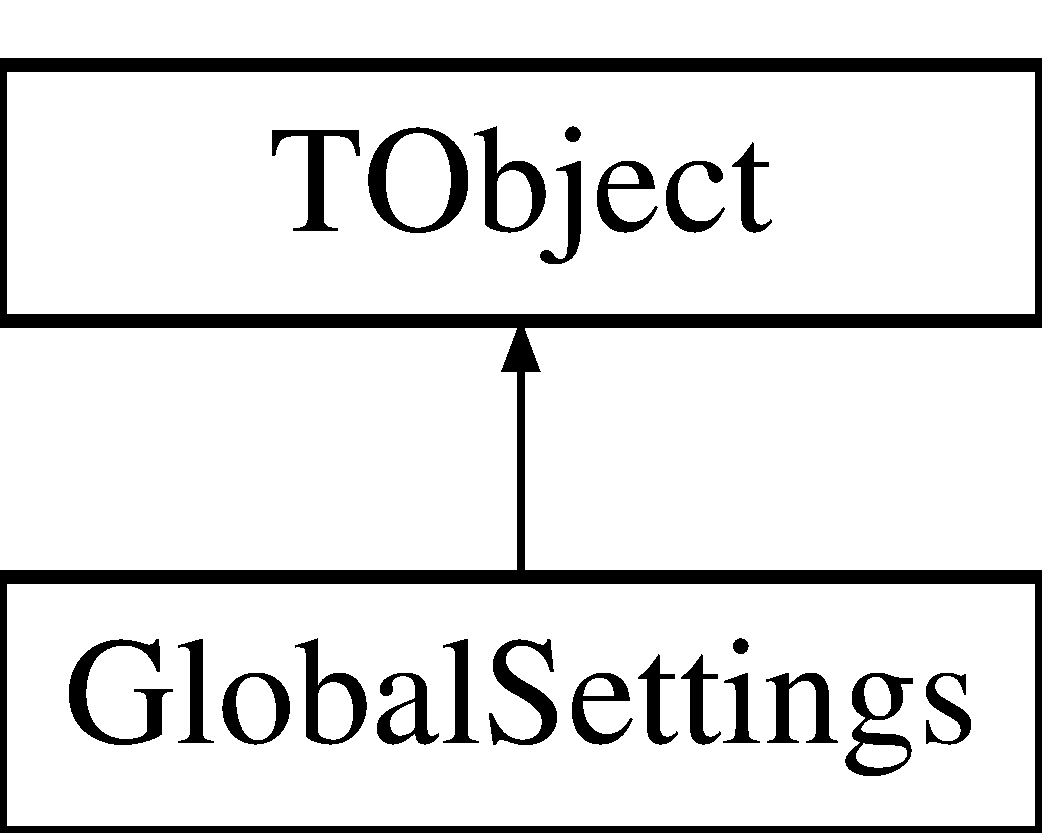
\includegraphics[height=2.000000cm]{class_global_settings}
\end{center}
\end{figure}
\subsection*{Public Member Functions}
\begin{DoxyCompactItemize}
\item 
\hypertarget{class_global_settings_a1c225d218e6d03979215f1a6204b7f4e}{{\bfseries Global\-Settings} (unsigned int, char $\ast$\mbox{[}$\,$\mbox{]})}\label{class_global_settings_a1c225d218e6d03979215f1a6204b7f4e}

\item 
\hypertarget{class_global_settings_a52a1e1677bc201c6b39835356293d85d}{unsigned short {\bfseries First\-Miniball\-Dgf} ()}\label{class_global_settings_a52a1e1677bc201c6b39835356293d85d}

\item 
\hypertarget{class_global_settings_aaadd8c6a7a474f0b9553ba19188eb264}{unsigned short {\bfseries Last\-Miniball\-Dgf} ()}\label{class_global_settings_aaadd8c6a7a474f0b9553ba19188eb264}

\item 
\hypertarget{class_global_settings_af0ff7c615f313cb54022cf6b5ddcdd23}{unsigned short {\bfseries Beamdump\-Dgf} ()}\label{class_global_settings_af0ff7c615f313cb54022cf6b5ddcdd23}

\item 
\hypertarget{class_global_settings_ad422d73434ae2ccc7b26ffed75d4f569}{unsigned short {\bfseries First\-Adc} ()}\label{class_global_settings_ad422d73434ae2ccc7b26ffed75d4f569}

\item 
\hypertarget{class_global_settings_a0b452889afe332aad1be1e9a74b58f4d}{unsigned short {\bfseries Last\-Adc} ()}\label{class_global_settings_a0b452889afe332aad1be1e9a74b58f4d}

\item 
\hypertarget{class_global_settings_a5590e2efb7c185568d151cb7172b58bc}{unsigned short {\bfseries Bragg\-Chamber} ()}\label{class_global_settings_a5590e2efb7c185568d151cb7172b58bc}

\item 
\hypertarget{class_global_settings_ac68f6e40bcec64f60cbdff06de507771}{unsigned short {\bfseries Scaler} ()}\label{class_global_settings_ac68f6e40bcec64f60cbdff06de507771}

\item 
\hypertarget{class_global_settings_a039a4d8e7a31e0c29f555ac862bd249f}{unsigned short {\bfseries Pattern\-Unit} ()}\label{class_global_settings_a039a4d8e7a31e0c29f555ac862bd249f}

\item 
\hypertarget{class_global_settings_a216b8164c02a1de1d5437df565cb9485}{unsigned short {\bfseries First\-Dgf\-Scaler} ()}\label{class_global_settings_a216b8164c02a1de1d5437df565cb9485}

\item 
\hypertarget{class_global_settings_a808e23c6df71ad3156777d8f6e3232b4}{unsigned short {\bfseries Last\-Dgf\-Scaler} ()}\label{class_global_settings_a808e23c6df71ad3156777d8f6e3232b4}

\item 
\hypertarget{class_global_settings_ad3c488b383c9894b0f40747da7a32613}{unsigned short {\bfseries Number\-Of\-Dgf\-Modules} ()}\label{class_global_settings_ad3c488b383c9894b0f40747da7a32613}

\item 
\hypertarget{class_global_settings_a0036e842692c336fcd4fd918b180f708}{unsigned short {\bfseries Number\-Of\-Adc\-Modules} ()}\label{class_global_settings_a0036e842692c336fcd4fd918b180f708}

\item 
\hypertarget{class_global_settings_a7706b4e61b18ee710e025229b99002c6}{unsigned short {\bfseries Number\-Of\-Pattern\-Units} ()}\label{class_global_settings_a7706b4e61b18ee710e025229b99002c6}

\item 
\hypertarget{class_global_settings_a47372087c05f31209288e4cac4b1ce04}{unsigned short {\bfseries Number\-Of\-Dgf\-Channels} ()}\label{class_global_settings_a47372087c05f31209288e4cac4b1ce04}

\item 
\hypertarget{class_global_settings_a5d61c4fefad9ffe29a9a296641bf1f3c}{unsigned short {\bfseries Number\-Of\-Timestamp\-Modules} ()}\label{class_global_settings_a5d61c4fefad9ffe29a9a296641bf1f3c}

\item 
\hypertarget{class_global_settings_abb55f0b2ec5c870d739e86cbf9496b7d}{unsigned short {\bfseries Timestamp\-Module} (unsigned short Index)}\label{class_global_settings_abb55f0b2ec5c870d739e86cbf9496b7d}

\item 
\hypertarget{class_global_settings_a10705cb601c558b8a5e6bc6344eaa5ad}{double {\bfseries Timestamp\-Module\-Offset} (unsigned short Index)}\label{class_global_settings_a10705cb601c558b8a5e6bc6344eaa5ad}

\item 
\hypertarget{class_global_settings_aaab0288f44318a1ad732edabd1bdf2f4}{unsigned short {\bfseries Timestamp\-Channel} ()}\label{class_global_settings_aaab0288f44318a1ad732edabd1bdf2f4}

\item 
\hypertarget{class_global_settings_aa749f02a0a70decee11846ba3ceb044c}{unsigned short {\bfseries Number\-Of\-Adcs\-Per\-Timestamp\-Module} ()}\label{class_global_settings_aa749f02a0a70decee11846ba3ceb044c}

\item 
\hypertarget{class_global_settings_a71ac24fe36fc3f7cc2844bdfedb2ea72}{unsigned short {\bfseries Ebis\-T1\-And\-Super\-Cycle\-Module} ()}\label{class_global_settings_a71ac24fe36fc3f7cc2844bdfedb2ea72}

\item 
\hypertarget{class_global_settings_af9cbfd6c5cd67d7efb49f7c23ef4320b}{unsigned short {\bfseries Ebis\-Channel} ()}\label{class_global_settings_af9cbfd6c5cd67d7efb49f7c23ef4320b}

\item 
\hypertarget{class_global_settings_a02d32bf705627b6d8e878ee1e6c69912}{unsigned short {\bfseries T1\-Channel} ()}\label{class_global_settings_a02d32bf705627b6d8e878ee1e6c69912}

\item 
\hypertarget{class_global_settings_a6395f10d579a2fb086f72979322a9ca3}{unsigned short {\bfseries Super\-Cycle\-Channel} ()}\label{class_global_settings_a6395f10d579a2fb086f72979322a9ca3}

\item 
\hypertarget{class_global_settings_a8f3ef06ff28b68746bb18833c343bc15}{unsigned short {\bfseries Marabou\-Dgf\-Module\-Offset} ()}\label{class_global_settings_a8f3ef06ff28b68746bb18833c343bc15}

\item 
\hypertarget{class_global_settings_a2bffff3342768138d92eb4bba965de8f}{unsigned short {\bfseries Marabou\-Adc\-Module\-Offset} ()}\label{class_global_settings_a2bffff3342768138d92eb4bba965de8f}

\item 
\hypertarget{class_global_settings_a3a66dee38bb8974fe42269881f58e6f4}{unsigned short {\bfseries Marabou\-Pattern\-Unit\-Offset} ()}\label{class_global_settings_a3a66dee38bb8974fe42269881f58e6f4}

\item 
\hypertarget{class_global_settings_adaf6b3cb383cea55ee595422baf2d6a4}{long long {\bfseries First\-Event} ()}\label{class_global_settings_adaf6b3cb383cea55ee595422baf2d6a4}

\item 
\hypertarget{class_global_settings_ac34c73a865be96c6c21edcf6f99fc35e}{long long {\bfseries Last\-Event} ()}\label{class_global_settings_ac34c73a865be96c6c21edcf6f99fc35e}

\item 
\hypertarget{class_global_settings_a922a7140b177a6fc02509fe2e443732e}{int {\bfseries Verbose\-Level} ()}\label{class_global_settings_a922a7140b177a6fc02509fe2e443732e}

\item 
\hypertarget{class_global_settings_a76ba56132fe67495a9c5c3a041a48a08}{const char $\ast$ {\bfseries Med\-File} ()}\label{class_global_settings_a76ba56132fe67495a9c5c3a041a48a08}

\item 
\hypertarget{class_global_settings_adbe98db49b93666afb5d9cb76e671f79}{const char $\ast$ {\bfseries On\-Beam\-File} ()}\label{class_global_settings_adbe98db49b93666afb5d9cb76e671f79}

\item 
\hypertarget{class_global_settings_aeed9285f4c68b974c23a4db5d89f3ed5}{const char $\ast$ {\bfseries On\-Beam\-Background\-File} ()}\label{class_global_settings_aeed9285f4c68b974c23a4db5d89f3ed5}

\item 
\hypertarget{class_global_settings_a156b6901d18059153c65ee043b9077b2}{const char $\ast$ {\bfseries Off\-Beam\-File} ()}\label{class_global_settings_a156b6901d18059153c65ee043b9077b2}

\item 
\hypertarget{class_global_settings_a262856ae6329c24152ca5056e71f1f94}{const char $\ast$ {\bfseries Scaler\-File} ()}\label{class_global_settings_a262856ae6329c24152ca5056e71f1f94}

\item 
\hypertarget{class_global_settings_a1fd06f7b8b9818d1f86f290241d3c923}{bool {\bfseries Is\-Timestamp\-Module} (unsigned short Module\-Number)}\label{class_global_settings_a1fd06f7b8b9818d1f86f290241d3c923}

\item 
\hypertarget{class_global_settings_aaee3450f69d50e203651d31c2069955c}{bool {\bfseries Coincident} (long long time)}\label{class_global_settings_aaee3450f69d50e203651d31c2069955c}

\item 
\hypertarget{class_global_settings_a973a2930c1c9d1d3a5fffbeb0f91f1d2}{unsigned short {\bfseries Real\-Time\-Index} ()}\label{class_global_settings_a973a2930c1c9d1d3a5fffbeb0f91f1d2}

\item 
\hypertarget{class_global_settings_a8917b578821e73520f027890799cbc15}{unsigned short {\bfseries Run\-Time\-Index} ()}\label{class_global_settings_a8917b578821e73520f027890799cbc15}

\item 
\hypertarget{class_global_settings_ae67adcfbae5f32f70dbaccb354083599}{unsigned short {\bfseries G\-S\-L\-T\-Time\-Index} ()}\label{class_global_settings_ae67adcfbae5f32f70dbaccb354083599}

\item 
\hypertarget{class_global_settings_a16fcf54c004f5b2cf38aafd747fd8df3}{unsigned short {\bfseries Number\-Of\-Events\-Index} ()}\label{class_global_settings_a16fcf54c004f5b2cf38aafd747fd8df3}

\item 
\hypertarget{class_global_settings_a9832ff3e3e2c8ffdd743ecef761c29fb}{unsigned short {\bfseries Channel\-Indices\-Offset} (unsigned short channel)}\label{class_global_settings_a9832ff3e3e2c8ffdd743ecef761c29fb}

\item 
\hypertarget{class_global_settings_a7984f02f9041a1a053a5bb504814aff5}{unsigned short {\bfseries Live\-Time\-Index} ()}\label{class_global_settings_a7984f02f9041a1a053a5bb504814aff5}

\item 
\hypertarget{class_global_settings_a3045c1e47cf31b2a1f2cdd036d2983d1}{unsigned short {\bfseries Fast\-Peak\-Index} ()}\label{class_global_settings_a3045c1e47cf31b2a1f2cdd036d2983d1}

\item 
\hypertarget{class_global_settings_a736690f2a63bcdb18f04f9831a484240}{unsigned short {\bfseries Bragg\-Trace\-Length} ()}\label{class_global_settings_a736690f2a63bcdb18f04f9831a484240}

\item 
\hypertarget{class_global_settings_a111d8b0e788e3709b00702f3a7ae2728}{bool {\bfseries Source\-Run} ()}\label{class_global_settings_a111d8b0e788e3709b00702f3a7ae2728}

\item 
\hypertarget{class_global_settings_a49c569d0d122bff3736e8e3debbfd013}{bool {\bfseries Include\-Scaler} ()}\label{class_global_settings_a49c569d0d122bff3736e8e3debbfd013}

\item 
\hypertarget{class_global_settings_acfaa849a405a80e912b1c42c7b0c258c}{bool {\bfseries Mesytec\-Adc} ()}\label{class_global_settings_acfaa849a405a80e912b1c42c7b0c258c}

\item 
\hypertarget{class_global_settings_a4a48a1c192b77998f1b1111d73aeaf5a}{bool {\bfseries S\-P\-E\-D\-E\-Chamb} ()}\label{class_global_settings_a4a48a1c192b77998f1b1111d73aeaf5a}

\item 
\hypertarget{class_global_settings_a0451be00dc54ba72b862ba682399e5e2}{unsigned short {\bfseries Nof\-Caen\-Adc} ()}\label{class_global_settings_a0451be00dc54ba72b862ba682399e5e2}

\item 
\hypertarget{class_global_settings_a5fd349a287cbe0159fb24d4ae2264fbb}{unsigned short {\bfseries Type\-Of\-Setup} ()}\label{class_global_settings_a5fd349a287cbe0159fb24d4ae2264fbb}

\item 
\hypertarget{class_global_settings_ae3067cec604f4bf7692c2a635411ffa3}{unsigned short {\bfseries Ebis\-Window\-Lower\-Edge} ()}\label{class_global_settings_ae3067cec604f4bf7692c2a635411ffa3}

\item 
\hypertarget{class_global_settings_ad13bfa3edd5436f4096e52d742348da7}{unsigned short {\bfseries Ebis\-Window\-Upper\-Edge} ()}\label{class_global_settings_ad13bfa3edd5436f4096e52d742348da7}

\item 
\hypertarget{class_global_settings_a2b7b49aa025fef97a5c5bf50f7b181c7}{long long {\bfseries Dgf\-Init\-Delay} ()}\label{class_global_settings_a2b7b49aa025fef97a5c5bf50f7b181c7}

\item 
\hypertarget{class_global_settings_a7057529627ce885278a417a6b31634fd}{bool {\bfseries Verify} ()}\label{class_global_settings_a7057529627ce885278a417a6b31634fd}

\end{DoxyCompactItemize}
\subsection*{Protected Member Functions}
\begin{DoxyCompactItemize}
\item 
\hypertarget{class_global_settings_a4ff35326d7293d230edd31fbf67bb10b}{void {\bfseries Read\-Settings} ()}\label{class_global_settings_a4ff35326d7293d230edd31fbf67bb10b}

\item 
\hypertarget{class_global_settings_ac91eec1a20a1366ec4859dd06249cf6d}{void {\bfseries Read\-Unpacker\-Settings} ()}\label{class_global_settings_ac91eec1a20a1366ec4859dd06249cf6d}

\end{DoxyCompactItemize}
\subsection*{Protected Attributes}
\begin{DoxyCompactItemize}
\item 
\hypertarget{class_global_settings_a0229c81f45f4d106c152e7182c088d31}{string {\bfseries f\-Med\-File}}\label{class_global_settings_a0229c81f45f4d106c152e7182c088d31}

\item 
\hypertarget{class_global_settings_a56ef4c7a1b24bf82ec39b96d51a51a42}{string {\bfseries f\-On\-Beam\-File}}\label{class_global_settings_a56ef4c7a1b24bf82ec39b96d51a51a42}

\item 
\hypertarget{class_global_settings_a438a9df97896968e64cd47aea5c3d2dc}{string {\bfseries f\-On\-Beam\-Background\-File}}\label{class_global_settings_a438a9df97896968e64cd47aea5c3d2dc}

\item 
\hypertarget{class_global_settings_a16eaa9f75457600f89c827ef9c0caafb}{string {\bfseries f\-Off\-Beam\-File}}\label{class_global_settings_a16eaa9f75457600f89c827ef9c0caafb}

\item 
\hypertarget{class_global_settings_a4569000d66e6974cc1546d5b89352391}{string {\bfseries f\-Scaler\-File}}\label{class_global_settings_a4569000d66e6974cc1546d5b89352391}

\item 
\hypertarget{class_global_settings_a6059278a514f661ef1b22306270f988b}{string {\bfseries f\-Settings\-File}}\label{class_global_settings_a6059278a514f661ef1b22306270f988b}

\item 
\hypertarget{class_global_settings_a9f4513fef0dc435e73cdf28e8112c63a}{T\-Env $\ast$ {\bfseries f\-Settings}}\label{class_global_settings_a9f4513fef0dc435e73cdf28e8112c63a}

\item 
\hypertarget{class_global_settings_ad41fddb0a8d3c23d38ed111794212540}{int {\bfseries f\-Verbose\-Level}}\label{class_global_settings_ad41fddb0a8d3c23d38ed111794212540}

\item 
\hypertarget{class_global_settings_a72197a1647fac4aca768935a9597b198}{long long {\bfseries f\-First\-Event}}\label{class_global_settings_a72197a1647fac4aca768935a9597b198}

\item 
\hypertarget{class_global_settings_afd8cd3f57779575ca4ed73e33219f13f}{long long {\bfseries f\-Last\-Event}}\label{class_global_settings_afd8cd3f57779575ca4ed73e33219f13f}

\item 
\hypertarget{class_global_settings_a2d65be6baaa7277cd901556019e8460c}{unsigned short {\bfseries f\-First\-Miniball\-Dgf}}\label{class_global_settings_a2d65be6baaa7277cd901556019e8460c}

\item 
\hypertarget{class_global_settings_ae650a409541da5bf8cc67778d4e34845}{unsigned short {\bfseries f\-Last\-Miniball\-Dgf}}\label{class_global_settings_ae650a409541da5bf8cc67778d4e34845}

\item 
\hypertarget{class_global_settings_a76296bafe3844f4ee63b34b0b5c2600e}{unsigned short {\bfseries f\-Beamdump\-Dgf}}\label{class_global_settings_a76296bafe3844f4ee63b34b0b5c2600e}

\item 
\hypertarget{class_global_settings_aa70de9fe6e03b15d344f75d91f45b25b}{unsigned short {\bfseries f\-First\-Adc}}\label{class_global_settings_aa70de9fe6e03b15d344f75d91f45b25b}

\item 
\hypertarget{class_global_settings_a74d18d73a1b28ffe37f17877b5d2bf4f}{unsigned short {\bfseries f\-Last\-Adc}}\label{class_global_settings_a74d18d73a1b28ffe37f17877b5d2bf4f}

\item 
\hypertarget{class_global_settings_a95d6d5584cddb3d89a457db7359a9a9d}{unsigned short {\bfseries f\-Bragg\-Chamber}}\label{class_global_settings_a95d6d5584cddb3d89a457db7359a9a9d}

\item 
\hypertarget{class_global_settings_ad4d098d925cc88a0a9e538648c3d2017}{unsigned short {\bfseries f\-Scaler}}\label{class_global_settings_ad4d098d925cc88a0a9e538648c3d2017}

\item 
\hypertarget{class_global_settings_a1d66578500af2f9b423a0d34ebf9bea6}{unsigned short {\bfseries f\-Pattern\-Unit}}\label{class_global_settings_a1d66578500af2f9b423a0d34ebf9bea6}

\item 
\hypertarget{class_global_settings_a0a209cc9dbb3763e646b9c61a43a6637}{unsigned short {\bfseries f\-First\-Dgf\-Scaler}}\label{class_global_settings_a0a209cc9dbb3763e646b9c61a43a6637}

\item 
\hypertarget{class_global_settings_aa397f932c6dc717b89f6e6b2dc740006}{unsigned short {\bfseries f\-Last\-Dgf\-Scaler}}\label{class_global_settings_aa397f932c6dc717b89f6e6b2dc740006}

\item 
\hypertarget{class_global_settings_aa4ea12bfdc34312dcb279bdf2efbcbb3}{double {\bfseries f\-Coincidence\-Window\-Width}}\label{class_global_settings_aa4ea12bfdc34312dcb279bdf2efbcbb3}

\item 
\hypertarget{class_global_settings_a83d940cc19cbd1a4df880d0f4bb9f7ab}{double {\bfseries f\-Reference\-Point\-Of\-Coincidence\-Window}}\label{class_global_settings_a83d940cc19cbd1a4df880d0f4bb9f7ab}

\item 
\hypertarget{class_global_settings_ad933baf31ffb6ce12452fb48e78aae9c}{long long {\bfseries f\-Lowest\-Coincidence}}\label{class_global_settings_ad933baf31ffb6ce12452fb48e78aae9c}

\item 
\hypertarget{class_global_settings_a8038987280b1ee7f8d4244c9f5c69020}{long long {\bfseries f\-Highest\-Coincidence}}\label{class_global_settings_a8038987280b1ee7f8d4244c9f5c69020}

\item 
\hypertarget{class_global_settings_a88d5191ef09e0c4889aaac6ce4f2efce}{unsigned short {\bfseries f\-Number\-Of\-Dgf\-Modules}}\label{class_global_settings_a88d5191ef09e0c4889aaac6ce4f2efce}

\item 
\hypertarget{class_global_settings_af5fac6b4659c9023f6bf3cdfb9d79b44}{unsigned short {\bfseries f\-Number\-Of\-Adc\-Modules}}\label{class_global_settings_af5fac6b4659c9023f6bf3cdfb9d79b44}

\item 
\hypertarget{class_global_settings_a6d3aad60ff241be473e4fef0eb9575fd}{unsigned short {\bfseries f\-Number\-Of\-Pattern\-Units}}\label{class_global_settings_a6d3aad60ff241be473e4fef0eb9575fd}

\item 
\hypertarget{class_global_settings_a19360b8664f3baa1adcf6b8252f45d35}{unsigned short {\bfseries f\-Number\-Of\-Dgf\-Channels}}\label{class_global_settings_a19360b8664f3baa1adcf6b8252f45d35}

\item 
\hypertarget{class_global_settings_ae3d4548748ddb92df4cdb1690a99cb34}{unsigned short {\bfseries f\-Number\-Of\-Adcs\-Per\-Timestamp\-Module}}\label{class_global_settings_ae3d4548748ddb92df4cdb1690a99cb34}

\item 
\hypertarget{class_global_settings_af1c870cfde3e88bf42fb5db20301863a}{unsigned short {\bfseries f\-Number\-Of\-Timestamp\-Modules}}\label{class_global_settings_af1c870cfde3e88bf42fb5db20301863a}

\item 
\hypertarget{class_global_settings_a70bc89b24c2c6b9cc95090efd2c71c2e}{unsigned short $\ast$ {\bfseries f\-Timestamp\-Module}}\label{class_global_settings_a70bc89b24c2c6b9cc95090efd2c71c2e}

\item 
\hypertarget{class_global_settings_a97d325770bf95368ee70d0e336032cc6}{double $\ast$ \hyperlink{class_global_settings_a97d325770bf95368ee70d0e336032cc6}{f\-Timestamp\-Module\-Offset}}\label{class_global_settings_a97d325770bf95368ee70d0e336032cc6}

\begin{DoxyCompactList}\small\item\em f\-Number\-Of\-Timestamp\-Modules \end{DoxyCompactList}\item 
\hypertarget{class_global_settings_abc63389c34c21eba6a25723442e825a2}{unsigned short \hyperlink{class_global_settings_abc63389c34c21eba6a25723442e825a2}{f\-Timestamp\-Channel}}\label{class_global_settings_abc63389c34c21eba6a25723442e825a2}

\begin{DoxyCompactList}\small\item\em f\-Number\-Of\-Timestamp\-Modules \end{DoxyCompactList}\item 
\hypertarget{class_global_settings_a0f85aaa3aa19f24ab7b3b029feb19e89}{unsigned short {\bfseries f\-Ebis\-T1\-And\-Super\-Cycle\-Module}}\label{class_global_settings_a0f85aaa3aa19f24ab7b3b029feb19e89}

\item 
\hypertarget{class_global_settings_a1e0af52a3df16678c85730eb93eec4b8}{unsigned short {\bfseries f\-Ebis\-Channel}}\label{class_global_settings_a1e0af52a3df16678c85730eb93eec4b8}

\item 
\hypertarget{class_global_settings_a8342c6229c94c09f5cd7cb57c69227f1}{unsigned short {\bfseries f\-T1\-Channel}}\label{class_global_settings_a8342c6229c94c09f5cd7cb57c69227f1}

\item 
\hypertarget{class_global_settings_a151bdb446baeac778c83c3df8ff97c71}{unsigned short {\bfseries f\-Super\-Cycle\-Channel}}\label{class_global_settings_a151bdb446baeac778c83c3df8ff97c71}

\item 
\hypertarget{class_global_settings_ae4982fffd750facbbe9562801711b25f}{unsigned short {\bfseries f\-Marabou\-Dgf\-Module\-Offset}}\label{class_global_settings_ae4982fffd750facbbe9562801711b25f}

\item 
\hypertarget{class_global_settings_acf1502561adce6da14a91b9b90f4d0fc}{unsigned short {\bfseries f\-Marabou\-Adc\-Module\-Offset}}\label{class_global_settings_acf1502561adce6da14a91b9b90f4d0fc}

\item 
\hypertarget{class_global_settings_a1275e401d46401ca89fc32e293642415}{unsigned short {\bfseries f\-Marabou\-Pattern\-Unit\-Offset}}\label{class_global_settings_a1275e401d46401ca89fc32e293642415}

\item 
\hypertarget{class_global_settings_a142b843d3d046e74845672a8177c9de1}{unsigned short {\bfseries f\-Real\-Time\-Index}}\label{class_global_settings_a142b843d3d046e74845672a8177c9de1}

\item 
\hypertarget{class_global_settings_afcd06d4313aede9d4d55fde8c90a6d7f}{unsigned short {\bfseries f\-Run\-Time\-Index}}\label{class_global_settings_afcd06d4313aede9d4d55fde8c90a6d7f}

\item 
\hypertarget{class_global_settings_af6209578839870c7608b5cecbcfc0bd8}{unsigned short {\bfseries f\-G\-S\-L\-T\-Time\-Index}}\label{class_global_settings_af6209578839870c7608b5cecbcfc0bd8}

\item 
\hypertarget{class_global_settings_a0a695f74fb8fb13a7212c03cc1c90d45}{unsigned short {\bfseries f\-Number\-Of\-Events\-Index}}\label{class_global_settings_a0a695f74fb8fb13a7212c03cc1c90d45}

\item 
\hypertarget{class_global_settings_a7b7fde75713d340b0c08b69cf52629b5}{unsigned short $\ast$ {\bfseries f\-Channel\-Indices\-Offset}}\label{class_global_settings_a7b7fde75713d340b0c08b69cf52629b5}

\item 
\hypertarget{class_global_settings_af6b5925fc6dc199bd0859a1d4471f4fb}{unsigned short {\bfseries f\-Live\-Time\-Index}}\label{class_global_settings_af6b5925fc6dc199bd0859a1d4471f4fb}

\item 
\hypertarget{class_global_settings_a909c95bed26cb1703234e1d7bbee812e}{unsigned short {\bfseries f\-Fast\-Peak\-Index}}\label{class_global_settings_a909c95bed26cb1703234e1d7bbee812e}

\item 
\hypertarget{class_global_settings_ad6552c5816c5265d32f930c96cb05897}{unsigned short {\bfseries f\-Bragg\-Trace\-Length}}\label{class_global_settings_ad6552c5816c5265d32f930c96cb05897}

\item 
\hypertarget{class_global_settings_ab91214dfb8843edede96c9a0a6b43af4}{bool {\bfseries f\-Source\-Run}}\label{class_global_settings_ab91214dfb8843edede96c9a0a6b43af4}

\item 
\hypertarget{class_global_settings_a8f72ba223b743b631ef8a5d5326e2cc1}{bool {\bfseries f\-Include\-Scaler}}\label{class_global_settings_a8f72ba223b743b631ef8a5d5326e2cc1}

\item 
\hypertarget{class_global_settings_a07a745de62188ac45111e5a0a53ee2a5}{bool {\bfseries f\-Mesytec\-Adc}}\label{class_global_settings_a07a745de62188ac45111e5a0a53ee2a5}

\item 
\hypertarget{class_global_settings_a24efecbf225ff6579002125d0717581d}{bool {\bfseries f\-S\-P\-E\-D\-E\-Chamb}}\label{class_global_settings_a24efecbf225ff6579002125d0717581d}

\item 
\hypertarget{class_global_settings_a3a834ca5fe537c8ee1a6eaee52fedf24}{unsigned short {\bfseries f\-Nof\-Caen\-Adc}}\label{class_global_settings_a3a834ca5fe537c8ee1a6eaee52fedf24}

\item 
\hypertarget{class_global_settings_a7cfa68e7cba82725e43b12bcf85795fa}{unsigned short {\bfseries f\-Type\-Of\-Setup}}\label{class_global_settings_a7cfa68e7cba82725e43b12bcf85795fa}

\item 
\hypertarget{class_global_settings_a7ec5e9d460b0b4571c04ad7c6ae783ee}{unsigned short {\bfseries f\-Ebis\-Window\-Lower\-Edge}}\label{class_global_settings_a7ec5e9d460b0b4571c04ad7c6ae783ee}

\item 
\hypertarget{class_global_settings_a72672076f3067f6866a4843f51e5311f}{unsigned short {\bfseries f\-Ebis\-Window\-Upper\-Edge}}\label{class_global_settings_a72672076f3067f6866a4843f51e5311f}

\item 
\hypertarget{class_global_settings_abc519c30d68b6a40a89850064cda3c64}{long long {\bfseries f\-Dgf\-Init\-Delay}}\label{class_global_settings_abc519c30d68b6a40a89850064cda3c64}

\end{DoxyCompactItemize}
\subsection*{Friends}
\begin{DoxyCompactItemize}
\item 
\hypertarget{class_global_settings_ac6ab153308b559e7d080396b0fc7183b}{ostream \& {\bfseries operator$<$$<$} (ostream \&, const \hyperlink{class_global_settings}{Global\-Settings} \&)}\label{class_global_settings_ac6ab153308b559e7d080396b0fc7183b}

\end{DoxyCompactItemize}


The documentation for this class was generated from the following files\-:\begin{DoxyCompactItemize}
\item 
Med\-To\-Root/Global\-Settings.\-hh\item 
Med\-To\-Root/Global\-Settings.\-cc\end{DoxyCompactItemize}

\hypertarget{classhists}{}\section{hists Class Reference}
\label{classhists}\index{hists@{hists}}


A class for making Coulex analysis histograms.  




{\ttfamily \#include $<$hists.\+hh$>$}

\subsection*{Public Member Functions}
\begin{DoxyCompactItemize}
\item 
void \hyperlink{classhists_affb3dcaefba3b63d20bbe438030e2f81}{Initialise} (\hyperlink{classdoppler}{doppler} dc\+\_\+)
\item 
\mbox{\Hypertarget{classhists_a98cf7d91940c6d77105d07b0783399ee}\label{classhists_a98cf7d91940c6d77105d07b0783399ee}} 
void {\bfseries Set\+\_\+ppwin} (float user\+\_\+ppwin)
\item 
\mbox{\Hypertarget{classhists_ae986e831e139c9e7e5a4e327e864484d}\label{classhists_ae986e831e139c9e7e5a4e327e864484d}} 
void {\bfseries Set\+\_\+maxrecoil} (int user\+\_\+maxrecoil)
\item 
\mbox{\Hypertarget{classhists_acfb845682216224712565e7b8a1c3ce2}\label{classhists_acfb845682216224712565e7b8a1c3ce2}} 
void {\bfseries Set\+\_\+minrecoil} (int user\+\_\+minrecoil)
\item 
\mbox{\Hypertarget{classhists_a0cc07e066791f9e8925fbbcfdc00d723}\label{classhists_a0cc07e066791f9e8925fbbcfdc00d723}} 
void {\bfseries Fill1h} (float G\+En, float G\+Th, float G\+Ph, vector$<$ float $>$ G\+Cor\+\_\+\+G\+En, vector$<$ float $>$ G\+Cor\+\_\+\+G\+Th, vector$<$ float $>$ G\+Cor\+\_\+\+G\+Ph, vector$<$ int $>$ G\+Cor\+\_\+\+G\+Clu\+ID, vector$<$ float $>$ G\+Cor\+\_\+\+Gtd, bool electron, float P\+En, Int\+\_\+t Pann, Int\+\_\+t Psec, Int\+\_\+t Pquad, Int\+\_\+t T1T, float weight=1.\+0)
\item 
\mbox{\Hypertarget{classhists_a84e3dd3dc98652844bbfea63652eb280}\label{classhists_a84e3dd3dc98652844bbfea63652eb280}} 
void {\bfseries Fill2h} (float G\+En, float G\+Th, float G\+Ph, vector$<$ float $>$ G\+Cor\+\_\+\+G\+En, vector$<$ float $>$ G\+Cor\+\_\+\+G\+Th, vector$<$ float $>$ G\+Cor\+\_\+\+G\+Ph, vector$<$ int $>$ G\+Cor\+\_\+\+G\+Clu\+ID, vector$<$ float $>$ G\+Cor\+\_\+\+Gtd, bool electron, vector$<$ float $>$ P\+En, vector$<$ int $>$ Pann, vector$<$ int $>$ Psec, vector$<$ int $>$ Pquad, vector$<$ int $>$ Pptr, vector$<$ float $>$ td, float weight=1.\+0)
\item 
\mbox{\Hypertarget{classhists_a2129f29167f7fdb68978412d81030844}\label{classhists_a2129f29167f7fdb68978412d81030844}} 
void {\bfseries Fill\+Del2h} (float G\+En, float G\+Th, float G\+Ph, vector$<$ float $>$ P\+En, vector$<$ int $>$ Pann, vector$<$ int $>$ Psec, vector$<$ int $>$ Pquad, vector$<$ int $>$ Pptr, vector$<$ float $>$ td, float weight=1.\+0)
\item 
\mbox{\Hypertarget{classhists_af555a97407e075689f176db774c87da3}\label{classhists_af555a97407e075689f176db774c87da3}} 
void {\bfseries Fill\+Gam1h} (float G\+En, float G\+Th, float G\+Ph, float P\+En, Int\+\_\+t Pann, Int\+\_\+t Psec, Int\+\_\+t Pquad, Int\+\_\+t T1T, Int\+\_\+t cut, float weight=1.\+0)
\item 
\mbox{\Hypertarget{classhists_a37e85d4eeab8262c6809d003d83d220e}\label{classhists_a37e85d4eeab8262c6809d003d83d220e}} 
void {\bfseries Fill\+Gam2h} (float G\+En, float G\+Th, float G\+Ph, vector$<$ float $>$ P\+En, vector$<$ int $>$ Pann, vector$<$ int $>$ Psec, vector$<$ int $>$ Pquad, Int\+\_\+t Bptr, Int\+\_\+t Tptr, float weight=1.\+0)
\item 
\mbox{\Hypertarget{classhists_a5c04c8d7cdb40e45f7ba00464c6835e1}\label{classhists_a5c04c8d7cdb40e45f7ba00464c6835e1}} 
void {\bfseries Fill\+Elec1h} (float G\+En, float G\+Th, float G\+Ph, float P\+En, Int\+\_\+t Pann, Int\+\_\+t Psec, Int\+\_\+t Pquad, Int\+\_\+t cut, float weight=1.\+0)
\item 
\mbox{\Hypertarget{classhists_a1734b966a54b280c42524291ddcd60c8}\label{classhists_a1734b966a54b280c42524291ddcd60c8}} 
void {\bfseries Fill\+Elec2h} (float G\+En, float G\+Th, float G\+Ph, vector$<$ float $>$ P\+En, vector$<$ int $>$ Pann, vector$<$ int $>$ Psec, vector$<$ int $>$ Pquad, Int\+\_\+t Bptr, Int\+\_\+t Tptr, float weight=1.\+0)
\item 
\mbox{\Hypertarget{classhists_ae7189f12a2d600e8b58affcdc4816638}\label{classhists_ae7189f12a2d600e8b58affcdc4816638}} 
void {\bfseries Fill\+Gam\+Gam1h} (float G\+En, float G\+Th, float G\+Ph, vector$<$ float $>$ G\+Cor\+\_\+\+G\+En, vector$<$ float $>$ G\+Cor\+\_\+\+G\+Th, vector$<$ float $>$ G\+Cor\+\_\+\+G\+Ph, vector$<$ int $>$ G\+Cor\+\_\+\+G\+Clu\+ID, vector$<$ float $>$ G\+Cor\+\_\+\+Gtd, float P\+En, Int\+\_\+t Pann, Int\+\_\+t Psec, Int\+\_\+t Pquad, Int\+\_\+t T1T, Int\+\_\+t cut, float weight=1.\+0)
\item 
\mbox{\Hypertarget{classhists_a77c5d523f6064a42098c029ffaa0fbbc}\label{classhists_a77c5d523f6064a42098c029ffaa0fbbc}} 
void {\bfseries Fill\+Gam\+Gam2h} (float G\+En, float G\+Th, float G\+Ph, vector$<$ float $>$ G\+Cor\+\_\+\+G\+En, vector$<$ float $>$ G\+Cor\+\_\+\+G\+Th, vector$<$ float $>$ G\+Cor\+\_\+\+G\+Ph, vector$<$ int $>$ G\+Cor\+\_\+\+G\+Clu\+ID, vector$<$ float $>$ G\+Cor\+\_\+\+Gtd, vector$<$ float $>$ P\+En, vector$<$ int $>$ Pann, vector$<$ int $>$ Psec, vector$<$ int $>$ Pquad, Int\+\_\+t Bptr, Int\+\_\+t Tptr, float weight=1.\+0)
\item 
\mbox{\Hypertarget{classhists_a618651882b77d410480e624dfd4b8ee4}\label{classhists_a618651882b77d410480e624dfd4b8ee4}} 
void {\bfseries Fill\+Par1h} (float P\+En, Int\+\_\+t Pann, Int\+\_\+t Psec, Int\+\_\+t Pquad, Int\+\_\+t cut, float weight=1.\+0)
\item 
\mbox{\Hypertarget{classhists_abdb2e69023e9fdd9080bcef611c26125}\label{classhists_abdb2e69023e9fdd9080bcef611c26125}} 
void {\bfseries Fill\+Par2h} (vector$<$ float $>$ P\+En, vector$<$ int $>$ Pann, vector$<$ int $>$ Psec, vector$<$ int $>$ Pquad, Int\+\_\+t Bptr, Int\+\_\+t Tptr, float weight=1.\+0)
\item 
\mbox{\Hypertarget{classhists_ab48ef7120a82723ec1db8fde8143d532}\label{classhists_ab48ef7120a82723ec1db8fde8143d532}} 
void {\bfseries Phi\+Cal\+Hists} (float G\+En, float G\+Th, float G\+Ph, float P\+En, Int\+\_\+t Pann, Int\+\_\+t Psec, Int\+\_\+t Pquad, Int\+\_\+t cut, float weight=1.\+0)
\item 
\mbox{\Hypertarget{classhists_a52b2233e6775d4a9bf714368101116cb}\label{classhists_a52b2233e6775d4a9bf714368101116cb}} 
void {\bfseries Add\+Spectra} (float bg\+\_\+frac)
\end{DoxyCompactItemize}
\subsection*{Public Attributes}
\begin{DoxyCompactItemize}
\item 
\mbox{\Hypertarget{classhists_a41afed096ec22360010c5394780ae311}\label{classhists_a41afed096ec22360010c5394780ae311}} 
T\+H1F $\ast$ {\bfseries p}
\item 
\mbox{\Hypertarget{classhists_aff8415e0daed67934f5b5d22dc2833e9}\label{classhists_aff8415e0daed67934f5b5d22dc2833e9}} 
T\+H1F $\ast$ {\bfseries r}
\item 
\mbox{\Hypertarget{classhists_a7deeb53d1622c43f1de1459c37554181}\label{classhists_a7deeb53d1622c43f1de1459c37554181}} 
T\+H1F $\ast$ {\bfseries pmr}
\item 
\mbox{\Hypertarget{classhists_a7e962900e2acf6aad5a34b37e8f7120b}\label{classhists_a7e962900e2acf6aad5a34b37e8f7120b}} 
T\+H1F $\ast$ {\bfseries pB}
\item 
\mbox{\Hypertarget{classhists_ade9c18d36c628ca168263749aec46881}\label{classhists_ade9c18d36c628ca168263749aec46881}} 
T\+H1F $\ast$ {\bfseries rB}
\item 
\mbox{\Hypertarget{classhists_a0ebe4e7e00a621e903d2badca471bb76}\label{classhists_a0ebe4e7e00a621e903d2badca471bb76}} 
T\+H1F $\ast$ {\bfseries p\+BmrB}
\item 
\mbox{\Hypertarget{classhists_a37b47338868009d91a4a9faee7d00d44}\label{classhists_a37b47338868009d91a4a9faee7d00d44}} 
T\+H1F $\ast$ {\bfseries pT}
\item 
\mbox{\Hypertarget{classhists_a61cf4fec0530bd16c881acc84a9f74d6}\label{classhists_a61cf4fec0530bd16c881acc84a9f74d6}} 
T\+H1F $\ast$ {\bfseries rT}
\item 
\mbox{\Hypertarget{classhists_a7e36a011237a42752b9f0e7b464925a8}\label{classhists_a7e36a011237a42752b9f0e7b464925a8}} 
T\+H1F $\ast$ {\bfseries p\+TmrT}
\item 
\mbox{\Hypertarget{classhists_ab1c1ddba953f87c0f4c32279bc9485d6}\label{classhists_ab1c1ddba953f87c0f4c32279bc9485d6}} 
T\+H1F $\ast$ {\bfseries p\+\_\+1B}
\item 
\mbox{\Hypertarget{classhists_ad287fcf0e40907decc131b3bcbb7ff08}\label{classhists_ad287fcf0e40907decc131b3bcbb7ff08}} 
T\+H1F $\ast$ {\bfseries r\+\_\+1B}
\item 
\mbox{\Hypertarget{classhists_ab0877e25719159c845f5134b66d8ef57}\label{classhists_ab0877e25719159c845f5134b66d8ef57}} 
T\+H1F $\ast$ {\bfseries p\+\_\+1T}
\item 
\mbox{\Hypertarget{classhists_a1db74575f897e684a6804016693861fd}\label{classhists_a1db74575f897e684a6804016693861fd}} 
T\+H1F $\ast$ {\bfseries r\+\_\+1T}
\item 
\mbox{\Hypertarget{classhists_a96f09434083d6b3fb9b8052b08b17643}\label{classhists_a96f09434083d6b3fb9b8052b08b17643}} 
T\+H1F $\ast$ {\bfseries p\+\_\+2h}
\item 
\mbox{\Hypertarget{classhists_a0f6af1c5d39f69b9e8a28df700382047}\label{classhists_a0f6af1c5d39f69b9e8a28df700382047}} 
T\+H1F $\ast$ {\bfseries r\+\_\+2h}
\item 
\mbox{\Hypertarget{classhists_ada542533ecdbcc36eaa7733b7d192bdb}\label{classhists_ada542533ecdbcc36eaa7733b7d192bdb}} 
T\+H2F $\ast$ {\bfseries p\+\_\+thetaB}
\item 
\mbox{\Hypertarget{classhists_ac38f1333db23a835bb3162e1ff1ccafa}\label{classhists_ac38f1333db23a835bb3162e1ff1ccafa}} 
T\+H2F $\ast$ {\bfseries p\+\_\+thetaT}
\item 
\mbox{\Hypertarget{classhists_a38784e1a26bf1d7d3625e07267a39edc}\label{classhists_a38784e1a26bf1d7d3625e07267a39edc}} 
T\+H1F $\ast$ {\bfseries pe}
\item 
\mbox{\Hypertarget{classhists_a683ed63fe7bc1d75f1f43ef53a18a473}\label{classhists_a683ed63fe7bc1d75f1f43ef53a18a473}} 
T\+H1F $\ast$ {\bfseries re}
\item 
\mbox{\Hypertarget{classhists_a84b377f9c971abb452e4af055934afd7}\label{classhists_a84b377f9c971abb452e4af055934afd7}} 
T\+H1F $\ast$ {\bfseries pemre}
\item 
\mbox{\Hypertarget{classhists_aa3cbab005d2e14d98ef1e22a2e991863}\label{classhists_aa3cbab005d2e14d98ef1e22a2e991863}} 
T\+H1F $\ast$ {\bfseries peB}
\item 
\mbox{\Hypertarget{classhists_a217224a3af224d7b54d8bf19942153a1}\label{classhists_a217224a3af224d7b54d8bf19942153a1}} 
T\+H1F $\ast$ {\bfseries reB}
\item 
\mbox{\Hypertarget{classhists_ad4dc6071195357ea7cec65aba7a99fa3}\label{classhists_ad4dc6071195357ea7cec65aba7a99fa3}} 
T\+H1F $\ast$ {\bfseries pe\+BmreB}
\item 
\mbox{\Hypertarget{classhists_a36bbcea64843d1fbb69eb2cb51cd3c31}\label{classhists_a36bbcea64843d1fbb69eb2cb51cd3c31}} 
T\+H1F $\ast$ {\bfseries peT}
\item 
\mbox{\Hypertarget{classhists_a89fffb3d4e8ee537fb88a94c8b040ded}\label{classhists_a89fffb3d4e8ee537fb88a94c8b040ded}} 
T\+H1F $\ast$ {\bfseries reT}
\item 
\mbox{\Hypertarget{classhists_a92687e271de5c150483e7c9a236eb43d}\label{classhists_a92687e271de5c150483e7c9a236eb43d}} 
T\+H1F $\ast$ {\bfseries pe\+TmreT}
\item 
\mbox{\Hypertarget{classhists_ad5b4c13720b0d24f77276f21b8363c66}\label{classhists_ad5b4c13720b0d24f77276f21b8363c66}} 
T\+H1F $\ast$ {\bfseries pe\+\_\+1B}
\item 
\mbox{\Hypertarget{classhists_a7fc66687fab011b9305b4a9b8bad42cc}\label{classhists_a7fc66687fab011b9305b4a9b8bad42cc}} 
T\+H1F $\ast$ {\bfseries re\+\_\+1B}
\item 
\mbox{\Hypertarget{classhists_abb9a948a50137b233eaab46db1c939b4}\label{classhists_abb9a948a50137b233eaab46db1c939b4}} 
T\+H1F $\ast$ {\bfseries pe\+\_\+1T}
\item 
\mbox{\Hypertarget{classhists_a09da286251d9a799601e95df79c00624}\label{classhists_a09da286251d9a799601e95df79c00624}} 
T\+H1F $\ast$ {\bfseries re\+\_\+1T}
\item 
\mbox{\Hypertarget{classhists_aaca8b51e55fce8683cabce72396f75c0}\label{classhists_aaca8b51e55fce8683cabce72396f75c0}} 
T\+H1F $\ast$ {\bfseries pe\+\_\+2h}
\item 
\mbox{\Hypertarget{classhists_aede8b10a65057023b94985fc57c2ad9f}\label{classhists_aede8b10a65057023b94985fc57c2ad9f}} 
T\+H1F $\ast$ {\bfseries re\+\_\+2h}
\item 
\mbox{\Hypertarget{classhists_a7415fe201eb8c804c21b1bede89d1031}\label{classhists_a7415fe201eb8c804c21b1bede89d1031}} 
T\+H2F $\ast$ {\bfseries gg}
\item 
\mbox{\Hypertarget{classhists_a0d5d7d910d9fe3b09c69dc8a9e58423b}\label{classhists_a0d5d7d910d9fe3b09c69dc8a9e58423b}} 
T\+H2F $\ast$ {\bfseries ge}
\item 
\mbox{\Hypertarget{classhists_a099758376b68e59fc4365de6b839ef79}\label{classhists_a099758376b68e59fc4365de6b839ef79}} 
T\+H2F $\ast$ {\bfseries gg\+\_\+dcT}
\item 
\mbox{\Hypertarget{classhists_ae76bf0351de34acd70c8b0cb25ad1f05}\label{classhists_ae76bf0351de34acd70c8b0cb25ad1f05}} 
T\+H2F $\ast$ {\bfseries gg\+\_\+dcB}
\item 
\mbox{\Hypertarget{classhists_aa023bc009594c3bea6e7074d45035874}\label{classhists_aa023bc009594c3bea6e7074d45035874}} 
T\+H1F $\ast$ {\bfseries gg\+\_\+td}
\item 
\mbox{\Hypertarget{classhists_a1e251e4167b18b19eee933a9e6aff56d}\label{classhists_a1e251e4167b18b19eee933a9e6aff56d}} 
T\+H1F $\ast$ {\bfseries ge\+\_\+td}
\item 
\mbox{\Hypertarget{classhists_aa66b693d7743742be93fbe79a0febc98}\label{classhists_aa66b693d7743742be93fbe79a0febc98}} 
T\+H1F $\ast$ {\bfseries gcor\+\_\+size}
\item 
\mbox{\Hypertarget{classhists_a86eb4ab6281feb7f501a6c69dc71f560}\label{classhists_a86eb4ab6281feb7f501a6c69dc71f560}} 
T\+H1F $\ast$ {\bfseries B\+\_\+dcB}
\item 
\mbox{\Hypertarget{classhists_a582b4fae986b0b4030d93ef9d0b96210}\label{classhists_a582b4fae986b0b4030d93ef9d0b96210}} 
T\+H1F $\ast$ {\bfseries B\+\_\+dcT}
\item 
\mbox{\Hypertarget{classhists_a3d31c04f487d44044725733b9bc2f95b}\label{classhists_a3d31c04f487d44044725733b9bc2f95b}} 
T\+H1F $\ast$ {\bfseries B\+\_\+1hdcB}
\item 
\mbox{\Hypertarget{classhists_aa167222668767ecae417a2b5c4295277}\label{classhists_aa167222668767ecae417a2b5c4295277}} 
T\+H1F $\ast$ {\bfseries B\+\_\+1hdcT}
\item 
\mbox{\Hypertarget{classhists_a70bf7dad8001cafd0c4bc3421e9aaf64}\label{classhists_a70bf7dad8001cafd0c4bc3421e9aaf64}} 
T\+H1F $\ast$ {\bfseries T\+\_\+dcT}
\item 
\mbox{\Hypertarget{classhists_a944ccb48909ab1d1f535ce91ae9fdb12}\label{classhists_a944ccb48909ab1d1f535ce91ae9fdb12}} 
T\+H1F $\ast$ {\bfseries T\+\_\+dcB}
\item 
\mbox{\Hypertarget{classhists_a0451c79dac759b8218daf8bbfa0e02fd}\label{classhists_a0451c79dac759b8218daf8bbfa0e02fd}} 
T\+H1F $\ast$ {\bfseries T\+\_\+1hdcT}
\item 
\mbox{\Hypertarget{classhists_a112696b860a04538d5ad6a4d09564eb7}\label{classhists_a112696b860a04538d5ad6a4d09564eb7}} 
T\+H1F $\ast$ {\bfseries T\+\_\+1hdcB}
\item 
\mbox{\Hypertarget{classhists_a5b4907e3faa89bba351314cd355139a5}\label{classhists_a5b4907e3faa89bba351314cd355139a5}} 
T\+H1F $\ast$ {\bfseries B\+\_\+\+T1\+T\+\_\+dcB}
\item 
\mbox{\Hypertarget{classhists_a339c59a1da0331bd90ff7233144909ac}\label{classhists_a339c59a1da0331bd90ff7233144909ac}} 
T\+H1F $\ast$ {\bfseries B\+\_\+\+T1\+T\+\_\+dcT}
\item 
\mbox{\Hypertarget{classhists_ab9fa21da1f614c2fec8eb68c5e2c5473}\label{classhists_ab9fa21da1f614c2fec8eb68c5e2c5473}} 
T\+H1F $\ast$ {\bfseries T\+\_\+\+T1\+T\+\_\+dcB}
\item 
\mbox{\Hypertarget{classhists_a80614a6a56dab57a991cc06ae6132c68}\label{classhists_a80614a6a56dab57a991cc06ae6132c68}} 
T\+H1F $\ast$ {\bfseries T\+\_\+\+T1\+T\+\_\+dcT}
\item 
\mbox{\Hypertarget{classhists_ada60aa83ba9c6437607e77392508c783}\label{classhists_ada60aa83ba9c6437607e77392508c783}} 
T\+H1F $\ast$ {\bfseries B\+\_\+\+T1\+T\+\_\+dc\+B\+\_\+p}
\item 
\mbox{\Hypertarget{classhists_a14f74e41530b7005f8f6d5e8844893d1}\label{classhists_a14f74e41530b7005f8f6d5e8844893d1}} 
T\+H1F $\ast$ {\bfseries B\+\_\+\+T1\+T\+\_\+dc\+T\+\_\+p}
\item 
\mbox{\Hypertarget{classhists_a607aa67b6bb2420930a6fd2428199249}\label{classhists_a607aa67b6bb2420930a6fd2428199249}} 
T\+H1F $\ast$ {\bfseries T\+\_\+\+T1\+T\+\_\+dc\+B\+\_\+p}
\item 
\mbox{\Hypertarget{classhists_a8014ab96f05466212ca216abb7e4b0a5}\label{classhists_a8014ab96f05466212ca216abb7e4b0a5}} 
T\+H1F $\ast$ {\bfseries T\+\_\+\+T1\+T\+\_\+dc\+T\+\_\+p}
\item 
\mbox{\Hypertarget{classhists_a4f1835825c668d04a41e8f73c7d3f7a7}\label{classhists_a4f1835825c668d04a41e8f73c7d3f7a7}} 
T\+H1F $\ast$ {\bfseries B\+\_\+\+T1\+T\+\_\+dc\+B\+\_\+d}
\item 
\mbox{\Hypertarget{classhists_a5993f7ed0ac0b878356872d2252bc759}\label{classhists_a5993f7ed0ac0b878356872d2252bc759}} 
T\+H1F $\ast$ {\bfseries B\+\_\+\+T1\+T\+\_\+dc\+T\+\_\+d}
\item 
\mbox{\Hypertarget{classhists_a84afdb6b1f62db65df51291c0ce50704}\label{classhists_a84afdb6b1f62db65df51291c0ce50704}} 
T\+H1F $\ast$ {\bfseries T\+\_\+\+T1\+T\+\_\+dc\+B\+\_\+d}
\item 
\mbox{\Hypertarget{classhists_ab0ebd182a298ed554e906ccee9da47b0}\label{classhists_ab0ebd182a298ed554e906ccee9da47b0}} 
T\+H1F $\ast$ {\bfseries T\+\_\+\+T1\+T\+\_\+dc\+T\+\_\+d}
\item 
\mbox{\Hypertarget{classhists_a397d28ec3c9003601e27a72be08832e8}\label{classhists_a397d28ec3c9003601e27a72be08832e8}} 
T\+H1F $\ast$ {\bfseries T\+\_\+dc\+B\+\_\+x} \mbox{[}16\mbox{]}
\item 
\mbox{\Hypertarget{classhists_ada420e344b4313fcf19169ccc828bbd8}\label{classhists_ada420e344b4313fcf19169ccc828bbd8}} 
T\+H1F $\ast$ {\bfseries T\+\_\+dc\+T\+\_\+x} \mbox{[}16\mbox{]}
\item 
\mbox{\Hypertarget{classhists_a0d41f4be68d9f3120cb6e24248cf91d8}\label{classhists_a0d41f4be68d9f3120cb6e24248cf91d8}} 
T\+H1F $\ast$ {\bfseries B\+\_\+dc\+B\+\_\+x} \mbox{[}16\mbox{]}
\item 
\mbox{\Hypertarget{classhists_afa5394484ba2e15e132974095715f401}\label{classhists_afa5394484ba2e15e132974095715f401}} 
T\+H1F $\ast$ {\bfseries B\+\_\+dc\+T\+\_\+x} \mbox{[}16\mbox{]}
\item 
\mbox{\Hypertarget{classhists_acb0927cbb98334ced64232dfb54dbfd7}\label{classhists_acb0927cbb98334ced64232dfb54dbfd7}} 
T\+H1F $\ast$ {\bfseries T\+\_\+del\+\_\+2hdcB}
\item 
\mbox{\Hypertarget{classhists_a3302caaa171f28563fbebecae90f081c}\label{classhists_a3302caaa171f28563fbebecae90f081c}} 
T\+H1F $\ast$ {\bfseries T\+\_\+del\+\_\+2h}
\item 
\mbox{\Hypertarget{classhists_a589d893ec180d1dcab2285d73fefe596}\label{classhists_a589d893ec180d1dcab2285d73fefe596}} 
T\+H1F $\ast$ {\bfseries gam\+\_\+dcB}
\item 
\mbox{\Hypertarget{classhists_ad7399ed62a116c07b548d1883bfff87a}\label{classhists_ad7399ed62a116c07b548d1883bfff87a}} 
T\+H1F $\ast$ {\bfseries gam\+\_\+dcT}
\item 
\mbox{\Hypertarget{classhists_aafe1950ee56bc2d748e6c1bad0efb087}\label{classhists_aafe1950ee56bc2d748e6c1bad0efb087}} 
T\+H1F $\ast$ {\bfseries T\+\_\+2hdcB}
\item 
\mbox{\Hypertarget{classhists_a8430e2f9207758cd7474b270212084a5}\label{classhists_a8430e2f9207758cd7474b270212084a5}} 
T\+H1F $\ast$ {\bfseries T\+\_\+2hdcT}
\item 
\mbox{\Hypertarget{classhists_a8b729a1fa4bcec8cb959263dd26ecc1a}\label{classhists_a8b729a1fa4bcec8cb959263dd26ecc1a}} 
T\+H1F $\ast$ {\bfseries Be\+\_\+dcB}
\item 
\mbox{\Hypertarget{classhists_a246bff8d2acec6b368890d50e5d70ca2}\label{classhists_a246bff8d2acec6b368890d50e5d70ca2}} 
T\+H1F $\ast$ {\bfseries Be\+\_\+dcT}
\item 
\mbox{\Hypertarget{classhists_a6ace27c77387e53512e7917e475b749a}\label{classhists_a6ace27c77387e53512e7917e475b749a}} 
T\+H1F $\ast$ {\bfseries Be\+\_\+1hdcB}
\item 
\mbox{\Hypertarget{classhists_a35289a28e9980cd7971e08ee6d6da647}\label{classhists_a35289a28e9980cd7971e08ee6d6da647}} 
T\+H1F $\ast$ {\bfseries Be\+\_\+1hdcT}
\item 
\mbox{\Hypertarget{classhists_aac5cef0c9fde441ef7325726cd49473e}\label{classhists_aac5cef0c9fde441ef7325726cd49473e}} 
T\+H1F $\ast$ {\bfseries Te\+\_\+dcT}
\item 
\mbox{\Hypertarget{classhists_af369482ccb37e4edf67fcd63d0c6e295}\label{classhists_af369482ccb37e4edf67fcd63d0c6e295}} 
T\+H1F $\ast$ {\bfseries Te\+\_\+dcB}
\item 
\mbox{\Hypertarget{classhists_a1d4855a08c440ff07ecd3f18ad5603b7}\label{classhists_a1d4855a08c440ff07ecd3f18ad5603b7}} 
T\+H1F $\ast$ {\bfseries Te\+\_\+1hdcT}
\item 
\mbox{\Hypertarget{classhists_a19fd67734b4b1036e6a6aa39560d8054}\label{classhists_a19fd67734b4b1036e6a6aa39560d8054}} 
T\+H1F $\ast$ {\bfseries Te\+\_\+1hdcB}
\item 
\mbox{\Hypertarget{classhists_ace74fbe7d1fd4da03304b44570b8b202}\label{classhists_ace74fbe7d1fd4da03304b44570b8b202}} 
T\+H1F $\ast$ {\bfseries elec\+\_\+dcB}
\item 
\mbox{\Hypertarget{classhists_af52e5cbaceb5b0582b66088c0dc1ca4a}\label{classhists_af52e5cbaceb5b0582b66088c0dc1ca4a}} 
T\+H1F $\ast$ {\bfseries elec\+\_\+dcT}
\item 
\mbox{\Hypertarget{classhists_a9a8730b34e80ce14eb4ae247189a8c7c}\label{classhists_a9a8730b34e80ce14eb4ae247189a8c7c}} 
T\+H1F $\ast$ {\bfseries Te\+\_\+2hdcB}
\item 
\mbox{\Hypertarget{classhists_ad9f7525c27e8a4e08fd7eb105d1532e8}\label{classhists_ad9f7525c27e8a4e08fd7eb105d1532e8}} 
T\+H1F $\ast$ {\bfseries Te\+\_\+2hdcT}
\item 
\mbox{\Hypertarget{classhists_ae7e1965b191fa91a011c3bb916acf82b}\label{classhists_ae7e1965b191fa91a011c3bb916acf82b}} 
T\+H2F $\ast$ {\bfseries part}
\item 
\mbox{\Hypertarget{classhists_ab2f82ce8e6460f4e0cf66022745502aa}\label{classhists_ab2f82ce8e6460f4e0cf66022745502aa}} 
T\+H2F $\ast$ {\bfseries part1h}
\item 
\mbox{\Hypertarget{classhists_ab5362852b3ced1f0e00c238a53063c1d}\label{classhists_ab5362852b3ced1f0e00c238a53063c1d}} 
T\+H2F $\ast$ {\bfseries part2h}
\item 
\mbox{\Hypertarget{classhists_ace85a8bdaa8292638c88cc3109715f10}\label{classhists_ace85a8bdaa8292638c88cc3109715f10}} 
T\+H2F $\ast$ {\bfseries partQ} \mbox{[}4\mbox{]}
\item 
\mbox{\Hypertarget{classhists_ae81ebc27f2c1626c7eec69dd2b98cf9d}\label{classhists_ae81ebc27f2c1626c7eec69dd2b98cf9d}} 
T\+H2F $\ast$ {\bfseries part\+\_\+ann}
\item 
\mbox{\Hypertarget{classhists_aeb1100de77471c82b1e4b2bdef8e3bef}\label{classhists_aeb1100de77471c82b1e4b2bdef8e3bef}} 
T\+H2F $\ast$ {\bfseries Bh}
\item 
\mbox{\Hypertarget{classhists_a30113490acc3bd21c41cf91ec2d56d76}\label{classhists_a30113490acc3bd21c41cf91ec2d56d76}} 
T\+H2F $\ast$ {\bfseries Th}
\item 
\mbox{\Hypertarget{classhists_aaf841cb978d167548cc0d6a7367b535b}\label{classhists_aaf841cb978d167548cc0d6a7367b535b}} 
T\+H2F $\ast$ {\bfseries B1h}
\item 
\mbox{\Hypertarget{classhists_a03b91f34a603432e8d38de2aeb6f4cb3}\label{classhists_a03b91f34a603432e8d38de2aeb6f4cb3}} 
T\+H2F $\ast$ {\bfseries T1h}
\item 
\mbox{\Hypertarget{classhists_a8bb22df02c23b6e1648a35e96f5b27cc}\label{classhists_a8bb22df02c23b6e1648a35e96f5b27cc}} 
T\+H2F $\ast$ {\bfseries B2h}
\item 
\mbox{\Hypertarget{classhists_ac609f6f35aeea5ef93bb3c3d0cb8879b}\label{classhists_ac609f6f35aeea5ef93bb3c3d0cb8879b}} 
T\+H2F $\ast$ {\bfseries T2h}
\item 
\mbox{\Hypertarget{classhists_ab5a2532e359cbaab3e455ea0402df683}\label{classhists_ab5a2532e359cbaab3e455ea0402df683}} 
T\+H2F $\ast$ {\bfseries Bhhigh}
\item 
\mbox{\Hypertarget{classhists_a1580aa18bfc6d03e70c9734923d5eb10}\label{classhists_a1580aa18bfc6d03e70c9734923d5eb10}} 
T\+H2F $\ast$ {\bfseries Bhlow}
\item 
\mbox{\Hypertarget{classhists_a2cde22029872705a43da498120e2aa46}\label{classhists_a2cde22029872705a43da498120e2aa46}} 
T\+H2F $\ast$ {\bfseries Thhigh}
\item 
\mbox{\Hypertarget{classhists_a83ece7e3db3b09a60a324ae5354f089a}\label{classhists_a83ece7e3db3b09a60a324ae5354f089a}} 
T\+H2F $\ast$ {\bfseries Thlow}
\item 
\mbox{\Hypertarget{classhists_abb4b732c26bc4427f87386c95bb62a20}\label{classhists_abb4b732c26bc4427f87386c95bb62a20}} 
T\+H1F $\ast$ {\bfseries target\+\_\+ev}
\item 
\mbox{\Hypertarget{classhists_a636d2dd2a4902718e73e85587c28bc18}\label{classhists_a636d2dd2a4902718e73e85587c28bc18}} 
T\+H1F $\ast$ {\bfseries target\+\_\+1pev}
\item 
\mbox{\Hypertarget{classhists_a7ceea5f78ab806205028fd01b9df235d}\label{classhists_a7ceea5f78ab806205028fd01b9df235d}} 
T\+H1F $\ast$ {\bfseries target\+\_\+2pev}
\item 
\mbox{\Hypertarget{classhists_a7de4d3c1ec119e5c1ac9ad96cfd58485}\label{classhists_a7de4d3c1ec119e5c1ac9ad96cfd58485}} 
T\+H2F $\ast$ {\bfseries Bsim}
\item 
\mbox{\Hypertarget{classhists_af47c4c518a3c97646fb692de05212086}\label{classhists_af47c4c518a3c97646fb692de05212086}} 
T\+H2F $\ast$ {\bfseries Tsim}
\item 
\mbox{\Hypertarget{classhists_a50d76c1d5471dd4655d40c4bffce89bf}\label{classhists_a50d76c1d5471dd4655d40c4bffce89bf}} 
T\+H2F $\ast$ {\bfseries en2hit}
\item 
\mbox{\Hypertarget{classhists_ae1df19b4b0de2ef60bf0cb58fb9c0b56}\label{classhists_ae1df19b4b0de2ef60bf0cb58fb9c0b56}} 
T\+H1F $\ast$ {\bfseries sum2hit}
\item 
\mbox{\Hypertarget{classhists_a9c5e347a9931ee406478680141938d93}\label{classhists_a9c5e347a9931ee406478680141938d93}} 
T\+H2F $\ast$ {\bfseries cdpic}
\item 
\mbox{\Hypertarget{classhists_aa3df083b17a09fe124f4ad32f23d116e}\label{classhists_aa3df083b17a09fe124f4ad32f23d116e}} 
T\+H1F $\ast$ {\bfseries multp}
\item 
\mbox{\Hypertarget{classhists_a3138630b94f51fbc6a2c84948c7c5cf2}\label{classhists_a3138630b94f51fbc6a2c84948c7c5cf2}} 
T\+H1F $\ast$ {\bfseries multr}
\item 
\mbox{\Hypertarget{classhists_ab3464ad4ba0e82d4108789becdea342c}\label{classhists_ab3464ad4ba0e82d4108789becdea342c}} 
T\+H1F $\ast$ {\bfseries velo}
\item 
\mbox{\Hypertarget{classhists_afb649b071eb30cbfb186f01d0371e983}\label{classhists_afb649b071eb30cbfb186f01d0371e983}} 
T\+H1F $\ast$ {\bfseries velo2}
\item 
\mbox{\Hypertarget{classhists_abaa6cc7052aaa0266712384d8394a3ca}\label{classhists_abaa6cc7052aaa0266712384d8394a3ca}} 
T\+H1F $\ast$ {\bfseries Ge\+Reject}
\item 
\mbox{\Hypertarget{classhists_a066fbbd2e0986d9ad91c72346d1251c9}\label{classhists_a066fbbd2e0986d9ad91c72346d1251c9}} 
T\+H1F $\ast$ {\bfseries Ge\+Pass}
\item 
\mbox{\Hypertarget{classhists_aaf12202a300bdc1e0fb2bb063219affd}\label{classhists_aaf12202a300bdc1e0fb2bb063219affd}} 
T\+H1F $\ast$ {\bfseries Ge\+Ratio}
\item 
\mbox{\Hypertarget{classhists_a64d2d67243f4540a785b531368e77db7}\label{classhists_a64d2d67243f4540a785b531368e77db7}} 
T\+H2F $\ast$ {\bfseries Ge\+Ang}
\item 
\mbox{\Hypertarget{classhists_a1db79da5d62b864a00edba35164ce62b}\label{classhists_a1db79da5d62b864a00edba35164ce62b}} 
T\+H1F $\ast$ {\bfseries tdiff}
\item 
\mbox{\Hypertarget{classhists_a307ef470870c3062b94931a75e45d72e}\label{classhists_a307ef470870c3062b94931a75e45d72e}} 
T\+H1F $\ast$ {\bfseries tdiff\+\_\+e}
\item 
\mbox{\Hypertarget{classhists_a83382e0f0012d20a168b327e608ab6dc}\label{classhists_a83382e0f0012d20a168b327e608ab6dc}} 
float {\bfseries tegate} \mbox{[}4\mbox{]}
\item 
\mbox{\Hypertarget{classhists_a034f8db2fb5bbc3799a21c972875d8dc}\label{classhists_a034f8db2fb5bbc3799a21c972875d8dc}} 
T\+H1F $\ast$ {\bfseries tdiffE} \mbox{[}4\mbox{]}
\item 
\mbox{\Hypertarget{classhists_ac86bf3c25b09b83c0d8efa3832671a23}\label{classhists_ac86bf3c25b09b83c0d8efa3832671a23}} 
T\+H1F $\ast$ {\bfseries tdiffQ} \mbox{[}4\mbox{]}
\item 
\mbox{\Hypertarget{classhists_a882cee022acf8051bd5c18b0177dcd5e}\label{classhists_a882cee022acf8051bd5c18b0177dcd5e}} 
T\+H1F $\ast$ {\bfseries tppdiff}
\item 
\mbox{\Hypertarget{classhists_aa38f4682a254eb6873d3ad87677f5275}\label{classhists_aa38f4682a254eb6873d3ad87677f5275}} 
T\+H2F $\ast$ {\bfseries tpp}
\item 
\mbox{\Hypertarget{classhists_ad4f783d5dd26a2fb7c4c314035710688}\label{classhists_ad4f783d5dd26a2fb7c4c314035710688}} 
T\+H1F $\ast$ {\bfseries t\+QQ} \mbox{[}2\mbox{]}
\item 
\mbox{\Hypertarget{classhists_af469b4438ba88b1af6df026c9dff4928}\label{classhists_af469b4438ba88b1af6df026c9dff4928}} 
float {\bfseries ppwin}
\item 
\mbox{\Hypertarget{classhists_aee1035f05bda36071913fc087f8ef80f}\label{classhists_aee1035f05bda36071913fc087f8ef80f}} 
int {\bfseries maxrecoil}
\item 
\mbox{\Hypertarget{classhists_ab46b91f1c6cbd9bff55649ee709a95e8}\label{classhists_ab46b91f1c6cbd9bff55649ee709a95e8}} 
int {\bfseries minrecoil}
\item 
\mbox{\Hypertarget{classhists_af9ae33bfde7848988faf5941f429d404}\label{classhists_af9ae33bfde7848988faf5941f429d404}} 
double {\bfseries cd\+\_\+angles} \mbox{[}17\mbox{]}
\item 
\mbox{\Hypertarget{classhists_a5bb6611932e44875a143ccd7812ce712}\label{classhists_a5bb6611932e44875a143ccd7812ce712}} 
\hyperlink{classdoppler}{doppler} {\bfseries dc}
\end{DoxyCompactItemize}


\subsection{Detailed Description}
A class for making Coulex analysis histograms. 

The hists class is used to define all histograms for the analysis. Crucially it defines a set of functions to be called, rather than filling each histogram individually with every call in \hyperlink{classg__clx_a9d5de859df4bfbb746726661ff1d24a9}{g\+\_\+clx\+::\+Loop}. This has the advantage of not repeating fill commands and therefore reducing the potential for copy/paste errors. Please try to use these functions as much as is reasonably possible. 

\subsection{Member Function Documentation}
\mbox{\Hypertarget{classhists_affb3dcaefba3b63d20bbe438030e2f81}\label{classhists_affb3dcaefba3b63d20bbe438030e2f81}} 
\index{hists@{hists}!Initialise@{Initialise}}
\index{Initialise@{Initialise}!hists@{hists}}
\subsubsection{\texorpdfstring{Initialise()}{Initialise()}}
{\footnotesize\ttfamily void hists\+::\+Initialise (\begin{DoxyParamCaption}\item[{\hyperlink{classdoppler}{doppler}}]{dc\+\_\+ }\end{DoxyParamCaption})}

Initialise all of the histograms that you want to fill If you add a new one, be careful not to break your memory limit. This causes unknown behaviour and may not give any errors. In the best case, you have a segmentation violation and you cannot work out where it comes from... Try deleting some histograms. Whatever you do, make sure you declare them in \hyperlink{hists_8hh_source}{hists.\+hh} file. 

The documentation for this class was generated from the following files\+:\begin{DoxyCompactItemize}
\item 
C\+L\+X\+Ana/hists.\+hh\item 
C\+L\+X\+Ana/hists.\+cc\end{DoxyCompactItemize}

\hypertarget{class_m_b_geometry}{}\section{M\+B\+Geometry Class Reference}
\label{class_m_b_geometry}\index{M\+B\+Geometry@{M\+B\+Geometry}}


Functions to convert Miniball angles read from the frame.  




{\ttfamily \#include $<$M\+B\+Geometry.\+hh$>$}

\subsection*{Public Member Functions}
\begin{DoxyCompactItemize}
\item 
void \hyperlink{class_m_b_geometry_a4d98a38f0dc1ca6a4a73477dde5cdd8d}{Setup\+Cluster} ()
\item 
void \hyperlink{class_m_b_geometry_a93f157cebad3f63dbbefb5b08f3555af}{Setup\+Cluster} (double user\+\_\+theta, double user\+\_\+phi, double user\+\_\+alpha, double user\+\_\+r)
\item 
void \hyperlink{class_m_b_geometry_a9a2a8c9609141be92d7ba30e6087aa30}{Set\+Clu\+Theta} (double user\+\_\+theta)
\item 
void \hyperlink{class_m_b_geometry_a74142f84cf6317d52ae39c0e0ff8a87e}{Set\+Clu\+Phi} (double user\+\_\+phi)
\item 
void \hyperlink{class_m_b_geometry_a0d4868b0360a6e5534918a9813540015}{Set\+Clu\+Alpha} (double user\+\_\+alpha)
\item 
void \hyperlink{class_m_b_geometry_a292c4326421c78871667e91c3694ae35}{Set\+CluR} (double user\+\_\+r)
\item 
double \hyperlink{class_m_b_geometry_a42aa536f15017724812712b0f8a77c12}{Get\+Core\+Theta} (int core)
\item 
double \hyperlink{class_m_b_geometry_a39f685610ae0e68e547a46f8ef992599}{Get\+Core\+Phi} (int core)
\item 
double \hyperlink{class_m_b_geometry_a49cdf742a2902fc85f0b24dfffa554a8}{Get\+Seg\+Theta} (int core, int seg)
\item 
double \hyperlink{class_m_b_geometry_a575ddd6022d2d686a83ebce3195b6c50}{Get\+Seg\+Phi} (int core, int seg)
\item 
\mbox{\Hypertarget{class_m_b_geometry_af4adfb858000405b21f79a6bf10c3c37}\label{class_m_b_geometry_af4adfb858000405b21f79a6bf10c3c37}} 
double \hyperlink{class_m_b_geometry_af4adfb858000405b21f79a6bf10c3c37}{M\+B\+Theta} (T\+Vector3 \&v)
\begin{DoxyCompactList}\small\item\em Get theta of a vector in Miniball system (return deg) \end{DoxyCompactList}\item 
\mbox{\Hypertarget{class_m_b_geometry_a399568d67bb83801ef6a2dbe963a535e}\label{class_m_b_geometry_a399568d67bb83801ef6a2dbe963a535e}} 
double \hyperlink{class_m_b_geometry_a399568d67bb83801ef6a2dbe963a535e}{M\+B\+Phi} (T\+Vector3 \&v)
\begin{DoxyCompactList}\small\item\em Get phi of a vector in Miniball system (return deg) \end{DoxyCompactList}\item 
\mbox{\Hypertarget{class_m_b_geometry_afd393f9db7182de7fb19f0c934edb383}\label{class_m_b_geometry_afd393f9db7182de7fb19f0c934edb383}} 
double \hyperlink{class_m_b_geometry_afd393f9db7182de7fb19f0c934edb383}{True\+Theta} (T\+Vector3 \&v)
\begin{DoxyCompactList}\small\item\em Get true theta of a vector (return deg) \end{DoxyCompactList}\item 
\mbox{\Hypertarget{class_m_b_geometry_a718d9c7fcc4a5fb8b9ecaabdc7a0503f}\label{class_m_b_geometry_a718d9c7fcc4a5fb8b9ecaabdc7a0503f}} 
double \hyperlink{class_m_b_geometry_a718d9c7fcc4a5fb8b9ecaabdc7a0503f}{True\+Phi} (T\+Vector3 \&v)
\begin{DoxyCompactList}\small\item\em Get the true phi of a vector (return deg) \end{DoxyCompactList}\item 
\mbox{\Hypertarget{class_m_b_geometry_a4d98a38f0dc1ca6a4a73477dde5cdd8d}\label{class_m_b_geometry_a4d98a38f0dc1ca6a4a73477dde5cdd8d}} 
void {\bfseries Setup\+Cluster} ()
\item 
\mbox{\Hypertarget{class_m_b_geometry_a93f157cebad3f63dbbefb5b08f3555af}\label{class_m_b_geometry_a93f157cebad3f63dbbefb5b08f3555af}} 
void {\bfseries Setup\+Cluster} (double user\+\_\+theta, double user\+\_\+phi, double user\+\_\+alpha, double user\+\_\+r)
\item 
\mbox{\Hypertarget{class_m_b_geometry_a9a2a8c9609141be92d7ba30e6087aa30}\label{class_m_b_geometry_a9a2a8c9609141be92d7ba30e6087aa30}} 
void {\bfseries Set\+Clu\+Theta} (double user\+\_\+theta)
\item 
\mbox{\Hypertarget{class_m_b_geometry_a74142f84cf6317d52ae39c0e0ff8a87e}\label{class_m_b_geometry_a74142f84cf6317d52ae39c0e0ff8a87e}} 
void {\bfseries Set\+Clu\+Phi} (double user\+\_\+phi)
\item 
\mbox{\Hypertarget{class_m_b_geometry_a0d4868b0360a6e5534918a9813540015}\label{class_m_b_geometry_a0d4868b0360a6e5534918a9813540015}} 
void {\bfseries Set\+Clu\+Alpha} (double user\+\_\+alpha)
\item 
\mbox{\Hypertarget{class_m_b_geometry_a292c4326421c78871667e91c3694ae35}\label{class_m_b_geometry_a292c4326421c78871667e91c3694ae35}} 
void {\bfseries Set\+CluR} (double user\+\_\+r)
\item 
\mbox{\Hypertarget{class_m_b_geometry_a42aa536f15017724812712b0f8a77c12}\label{class_m_b_geometry_a42aa536f15017724812712b0f8a77c12}} 
double {\bfseries Get\+Core\+Theta} (int core)
\item 
\mbox{\Hypertarget{class_m_b_geometry_a39f685610ae0e68e547a46f8ef992599}\label{class_m_b_geometry_a39f685610ae0e68e547a46f8ef992599}} 
double {\bfseries Get\+Core\+Phi} (int core)
\item 
\mbox{\Hypertarget{class_m_b_geometry_a49cdf742a2902fc85f0b24dfffa554a8}\label{class_m_b_geometry_a49cdf742a2902fc85f0b24dfffa554a8}} 
double {\bfseries Get\+Seg\+Theta} (int core, int seg)
\item 
\mbox{\Hypertarget{class_m_b_geometry_a575ddd6022d2d686a83ebce3195b6c50}\label{class_m_b_geometry_a575ddd6022d2d686a83ebce3195b6c50}} 
double {\bfseries Get\+Seg\+Phi} (int core, int seg)
\item 
\mbox{\Hypertarget{class_m_b_geometry_a4d98a38f0dc1ca6a4a73477dde5cdd8d}\label{class_m_b_geometry_a4d98a38f0dc1ca6a4a73477dde5cdd8d}} 
void {\bfseries Setup\+Cluster} ()
\item 
\mbox{\Hypertarget{class_m_b_geometry_a93f157cebad3f63dbbefb5b08f3555af}\label{class_m_b_geometry_a93f157cebad3f63dbbefb5b08f3555af}} 
void {\bfseries Setup\+Cluster} (double user\+\_\+theta, double user\+\_\+phi, double user\+\_\+alpha, double user\+\_\+r)
\item 
\mbox{\Hypertarget{class_m_b_geometry_a9a2a8c9609141be92d7ba30e6087aa30}\label{class_m_b_geometry_a9a2a8c9609141be92d7ba30e6087aa30}} 
void {\bfseries Set\+Clu\+Theta} (double user\+\_\+theta)
\item 
\mbox{\Hypertarget{class_m_b_geometry_a74142f84cf6317d52ae39c0e0ff8a87e}\label{class_m_b_geometry_a74142f84cf6317d52ae39c0e0ff8a87e}} 
void {\bfseries Set\+Clu\+Phi} (double user\+\_\+phi)
\item 
\mbox{\Hypertarget{class_m_b_geometry_a0d4868b0360a6e5534918a9813540015}\label{class_m_b_geometry_a0d4868b0360a6e5534918a9813540015}} 
void {\bfseries Set\+Clu\+Alpha} (double user\+\_\+alpha)
\item 
\mbox{\Hypertarget{class_m_b_geometry_a292c4326421c78871667e91c3694ae35}\label{class_m_b_geometry_a292c4326421c78871667e91c3694ae35}} 
void {\bfseries Set\+CluR} (double user\+\_\+r)
\item 
\mbox{\Hypertarget{class_m_b_geometry_a42aa536f15017724812712b0f8a77c12}\label{class_m_b_geometry_a42aa536f15017724812712b0f8a77c12}} 
double {\bfseries Get\+Core\+Theta} (int core)
\item 
\mbox{\Hypertarget{class_m_b_geometry_a39f685610ae0e68e547a46f8ef992599}\label{class_m_b_geometry_a39f685610ae0e68e547a46f8ef992599}} 
double {\bfseries Get\+Core\+Phi} (int core)
\item 
\mbox{\Hypertarget{class_m_b_geometry_a49cdf742a2902fc85f0b24dfffa554a8}\label{class_m_b_geometry_a49cdf742a2902fc85f0b24dfffa554a8}} 
double {\bfseries Get\+Seg\+Theta} (int core, int seg)
\item 
\mbox{\Hypertarget{class_m_b_geometry_a575ddd6022d2d686a83ebce3195b6c50}\label{class_m_b_geometry_a575ddd6022d2d686a83ebce3195b6c50}} 
double {\bfseries Get\+Seg\+Phi} (int core, int seg)
\item 
\mbox{\Hypertarget{class_m_b_geometry_af4adfb858000405b21f79a6bf10c3c37}\label{class_m_b_geometry_af4adfb858000405b21f79a6bf10c3c37}} 
double {\bfseries M\+B\+Theta} (T\+Vector3 \&v)
\item 
\mbox{\Hypertarget{class_m_b_geometry_a399568d67bb83801ef6a2dbe963a535e}\label{class_m_b_geometry_a399568d67bb83801ef6a2dbe963a535e}} 
double {\bfseries M\+B\+Phi} (T\+Vector3 \&v)
\item 
\mbox{\Hypertarget{class_m_b_geometry_afd393f9db7182de7fb19f0c934edb383}\label{class_m_b_geometry_afd393f9db7182de7fb19f0c934edb383}} 
double {\bfseries True\+Theta} (T\+Vector3 \&v)
\item 
\mbox{\Hypertarget{class_m_b_geometry_a718d9c7fcc4a5fb8b9ecaabdc7a0503f}\label{class_m_b_geometry_a718d9c7fcc4a5fb8b9ecaabdc7a0503f}} 
double {\bfseries True\+Phi} (T\+Vector3 \&v)
\end{DoxyCompactItemize}


\subsection{Detailed Description}
Functions to convert Miniball angles read from the frame. 



 \subsubsection*{Miniball Geometry class }

A geometry class that converts cluster angles read from the Miniball frame into real-\/life angles for the analysis. You can have theta and phi angles of the centres of each cluster, crystal and segment in frame geometry or true/beam geometry. 

\subsection{Member Function Documentation}
\mbox{\Hypertarget{class_m_b_geometry_a39f685610ae0e68e547a46f8ef992599}\label{class_m_b_geometry_a39f685610ae0e68e547a46f8ef992599}} 
\index{M\+B\+Geometry@{M\+B\+Geometry}!Get\+Core\+Phi@{Get\+Core\+Phi}}
\index{Get\+Core\+Phi@{Get\+Core\+Phi}!M\+B\+Geometry@{M\+B\+Geometry}}
\subsubsection{\texorpdfstring{Get\+Core\+Phi()}{GetCorePhi()}}
{\footnotesize\ttfamily double M\+B\+Geometry\+::\+Get\+Core\+Phi (\begin{DoxyParamCaption}\item[{int}]{core }\end{DoxyParamCaption})}

Get the phi angle of the core with respect to the beam \mbox{\Hypertarget{class_m_b_geometry_a42aa536f15017724812712b0f8a77c12}\label{class_m_b_geometry_a42aa536f15017724812712b0f8a77c12}} 
\index{M\+B\+Geometry@{M\+B\+Geometry}!Get\+Core\+Theta@{Get\+Core\+Theta}}
\index{Get\+Core\+Theta@{Get\+Core\+Theta}!M\+B\+Geometry@{M\+B\+Geometry}}
\subsubsection{\texorpdfstring{Get\+Core\+Theta()}{GetCoreTheta()}}
{\footnotesize\ttfamily double M\+B\+Geometry\+::\+Get\+Core\+Theta (\begin{DoxyParamCaption}\item[{int}]{core }\end{DoxyParamCaption})}

Get the theta angle of the core with respect to the beam \mbox{\Hypertarget{class_m_b_geometry_a575ddd6022d2d686a83ebce3195b6c50}\label{class_m_b_geometry_a575ddd6022d2d686a83ebce3195b6c50}} 
\index{M\+B\+Geometry@{M\+B\+Geometry}!Get\+Seg\+Phi@{Get\+Seg\+Phi}}
\index{Get\+Seg\+Phi@{Get\+Seg\+Phi}!M\+B\+Geometry@{M\+B\+Geometry}}
\subsubsection{\texorpdfstring{Get\+Seg\+Phi()}{GetSegPhi()}}
{\footnotesize\ttfamily double M\+B\+Geometry\+::\+Get\+Seg\+Phi (\begin{DoxyParamCaption}\item[{int}]{core,  }\item[{int}]{seg }\end{DoxyParamCaption})}

Get the phi angle of a segment with respect to the beam \mbox{\Hypertarget{class_m_b_geometry_a49cdf742a2902fc85f0b24dfffa554a8}\label{class_m_b_geometry_a49cdf742a2902fc85f0b24dfffa554a8}} 
\index{M\+B\+Geometry@{M\+B\+Geometry}!Get\+Seg\+Theta@{Get\+Seg\+Theta}}
\index{Get\+Seg\+Theta@{Get\+Seg\+Theta}!M\+B\+Geometry@{M\+B\+Geometry}}
\subsubsection{\texorpdfstring{Get\+Seg\+Theta()}{GetSegTheta()}}
{\footnotesize\ttfamily double M\+B\+Geometry\+::\+Get\+Seg\+Theta (\begin{DoxyParamCaption}\item[{int}]{core,  }\item[{int}]{seg }\end{DoxyParamCaption})}

Get the theta angle of a segment with respect to the beam \mbox{\Hypertarget{class_m_b_geometry_a0d4868b0360a6e5534918a9813540015}\label{class_m_b_geometry_a0d4868b0360a6e5534918a9813540015}} 
\index{M\+B\+Geometry@{M\+B\+Geometry}!Set\+Clu\+Alpha@{Set\+Clu\+Alpha}}
\index{Set\+Clu\+Alpha@{Set\+Clu\+Alpha}!M\+B\+Geometry@{M\+B\+Geometry}}
\subsubsection{\texorpdfstring{Set\+Clu\+Alpha()}{SetCluAlpha()}}
{\footnotesize\ttfamily void M\+B\+Geometry\+::\+Set\+Clu\+Alpha (\begin{DoxyParamCaption}\item[{double}]{user\+\_\+alpha }\end{DoxyParamCaption})}

Set the alpha angle measured from the frame \mbox{\Hypertarget{class_m_b_geometry_a74142f84cf6317d52ae39c0e0ff8a87e}\label{class_m_b_geometry_a74142f84cf6317d52ae39c0e0ff8a87e}} 
\index{M\+B\+Geometry@{M\+B\+Geometry}!Set\+Clu\+Phi@{Set\+Clu\+Phi}}
\index{Set\+Clu\+Phi@{Set\+Clu\+Phi}!M\+B\+Geometry@{M\+B\+Geometry}}
\subsubsection{\texorpdfstring{Set\+Clu\+Phi()}{SetCluPhi()}}
{\footnotesize\ttfamily void M\+B\+Geometry\+::\+Set\+Clu\+Phi (\begin{DoxyParamCaption}\item[{double}]{user\+\_\+phi }\end{DoxyParamCaption})}

Set the phi angle measured from the frame \mbox{\Hypertarget{class_m_b_geometry_a292c4326421c78871667e91c3694ae35}\label{class_m_b_geometry_a292c4326421c78871667e91c3694ae35}} 
\index{M\+B\+Geometry@{M\+B\+Geometry}!Set\+CluR@{Set\+CluR}}
\index{Set\+CluR@{Set\+CluR}!M\+B\+Geometry@{M\+B\+Geometry}}
\subsubsection{\texorpdfstring{Set\+Clu\+R()}{SetCluR()}}
{\footnotesize\ttfamily void M\+B\+Geometry\+::\+Set\+CluR (\begin{DoxyParamCaption}\item[{double}]{user\+\_\+r }\end{DoxyParamCaption})}

Set the distance between the target and face of the cluster \mbox{\Hypertarget{class_m_b_geometry_a9a2a8c9609141be92d7ba30e6087aa30}\label{class_m_b_geometry_a9a2a8c9609141be92d7ba30e6087aa30}} 
\index{M\+B\+Geometry@{M\+B\+Geometry}!Set\+Clu\+Theta@{Set\+Clu\+Theta}}
\index{Set\+Clu\+Theta@{Set\+Clu\+Theta}!M\+B\+Geometry@{M\+B\+Geometry}}
\subsubsection{\texorpdfstring{Set\+Clu\+Theta()}{SetCluTheta()}}
{\footnotesize\ttfamily void M\+B\+Geometry\+::\+Set\+Clu\+Theta (\begin{DoxyParamCaption}\item[{double}]{user\+\_\+theta }\end{DoxyParamCaption})}

Set the theta angle measured from the frame \mbox{\Hypertarget{class_m_b_geometry_a4d98a38f0dc1ca6a4a73477dde5cdd8d}\label{class_m_b_geometry_a4d98a38f0dc1ca6a4a73477dde5cdd8d}} 
\index{M\+B\+Geometry@{M\+B\+Geometry}!Setup\+Cluster@{Setup\+Cluster}}
\index{Setup\+Cluster@{Setup\+Cluster}!M\+B\+Geometry@{M\+B\+Geometry}}
\subsubsection{\texorpdfstring{Setup\+Cluster()}{SetupCluster()}\hspace{0.1cm}{\footnotesize\ttfamily [1/2]}}
{\footnotesize\ttfamily void M\+B\+Geometry\+::\+Setup\+Cluster (\begin{DoxyParamCaption}{ }\end{DoxyParamCaption})}

Setup cluster main routine \mbox{\Hypertarget{class_m_b_geometry_a93f157cebad3f63dbbefb5b08f3555af}\label{class_m_b_geometry_a93f157cebad3f63dbbefb5b08f3555af}} 
\index{M\+B\+Geometry@{M\+B\+Geometry}!Setup\+Cluster@{Setup\+Cluster}}
\index{Setup\+Cluster@{Setup\+Cluster}!M\+B\+Geometry@{M\+B\+Geometry}}
\subsubsection{\texorpdfstring{Setup\+Cluster()}{SetupCluster()}\hspace{0.1cm}{\footnotesize\ttfamily [2/2]}}
{\footnotesize\ttfamily void M\+B\+Geometry\+::\+Setup\+Cluster (\begin{DoxyParamCaption}\item[{double}]{user\+\_\+theta,  }\item[{double}]{user\+\_\+phi,  }\item[{double}]{user\+\_\+alpha,  }\item[{double}]{user\+\_\+r }\end{DoxyParamCaption})}

Setup the cluster with coordinate values 

The documentation for this class was generated from the following files\+:\begin{DoxyCompactItemize}
\item 
C\+L\+X\+Ana/M\+B\+Geometry.\+hh\item 
C\+L\+X\+Ana/M\+B\+Geometry.\+cc\item 
Mnt\+Ana/M\+B\+Geometry\+\_\+orig.\+cc\end{DoxyCompactItemize}

\input{class_particle_gamma_tree}
\hypertarget{class_particle_range}{}\section{Particle\+Range Class Reference}
\label{class_particle_range}\index{Particle\+Range@{Particle\+Range}}


Class for reading and interpolating range data from \textquotesingle{}zrange\textquotesingle{}.  




{\ttfamily \#include $<$Particle\+Range.\+hh$>$}

\subsection*{Public Member Functions}
\begin{DoxyCompactItemize}
\item 
\mbox{\Hypertarget{class_particle_range_a4273029166d7a6220bfd1728b6c18f69}\label{class_particle_range_a4273029166d7a6220bfd1728b6c18f69}} 
\hyperlink{class_particle_range_a4273029166d7a6220bfd1728b6c18f69}{Particle\+Range} ()
\begin{DoxyCompactList}\small\item\em Initialize values of Emin, Emax, Estep. \end{DoxyCompactList}\item 
void \hyperlink{class_particle_range_ac1e0da5aca629369e93caf8e883da624}{Read} (const std\+::string \&filename)
\begin{DoxyCompactList}\small\item\em Read an output file of zrange. \end{DoxyCompactList}\item 
float \hyperlink{class_particle_range_a433dead3f85fe19ee1675934b65acf3f}{Get\+Range} (int energy) const
\begin{DoxyCompactList}\small\item\em Get the range for a given particle energy. \end{DoxyCompactList}\end{DoxyCompactItemize}


\subsection{Detailed Description}
Class for reading and interpolating range data from \textquotesingle{}zrange\textquotesingle{}. 

\subsection{Member Function Documentation}
\mbox{\Hypertarget{class_particle_range_a433dead3f85fe19ee1675934b65acf3f}\label{class_particle_range_a433dead3f85fe19ee1675934b65acf3f}} 
\index{Particle\+Range@{Particle\+Range}!Get\+Range@{Get\+Range}}
\index{Get\+Range@{Get\+Range}!Particle\+Range@{Particle\+Range}}
\subsubsection{\texorpdfstring{Get\+Range()}{GetRange()}}
{\footnotesize\ttfamily float Particle\+Range\+::\+Get\+Range (\begin{DoxyParamCaption}\item[{int}]{energy }\end{DoxyParamCaption}) const}



Get the range for a given particle energy. 

If the energy is too high, 1m is returned. If it is to low, 0 is returned.

\begin{DoxyReturn}{Returns}
The range for this particle energy. 
\end{DoxyReturn}

\begin{DoxyParams}{Parameters}
{\em energy} & Particle energy in keV. \\
\hline
\end{DoxyParams}
\mbox{\Hypertarget{class_particle_range_ac1e0da5aca629369e93caf8e883da624}\label{class_particle_range_ac1e0da5aca629369e93caf8e883da624}} 
\index{Particle\+Range@{Particle\+Range}!Read@{Read}}
\index{Read@{Read}!Particle\+Range@{Particle\+Range}}
\subsubsection{\texorpdfstring{Read()}{Read()}}
{\footnotesize\ttfamily void Particle\+Range\+::\+Read (\begin{DoxyParamCaption}\item[{const std\+::string \&}]{filename }\end{DoxyParamCaption})}



Read an output file of zrange. 

These files have three columns\+: particle energy \mbox{[}MeV\mbox{]}, range \mbox{[}um\mbox{]}, and range uncertainty \mbox{[}um\mbox{]}. The zrange data are interpolated in Estep steps between Emin and Emax. 
\begin{DoxyParams}{Parameters}
{\em filename} & The name of the file to read. \\
\hline
\end{DoxyParams}


The documentation for this class was generated from the following files\+:\begin{DoxyCompactItemize}
\item 
Med\+To\+Root/Particle\+Range.\+hh\item 
Med\+To\+Root/Particle\+Range.\+cc\end{DoxyCompactItemize}

\hypertarget{class_pattern_unit}{\section{Pattern\-Unit Class Reference}
\label{class_pattern_unit}\index{Pattern\-Unit@{Pattern\-Unit}}
}
Inheritance diagram for Pattern\-Unit\-:\begin{figure}[H]
\begin{center}
\leavevmode
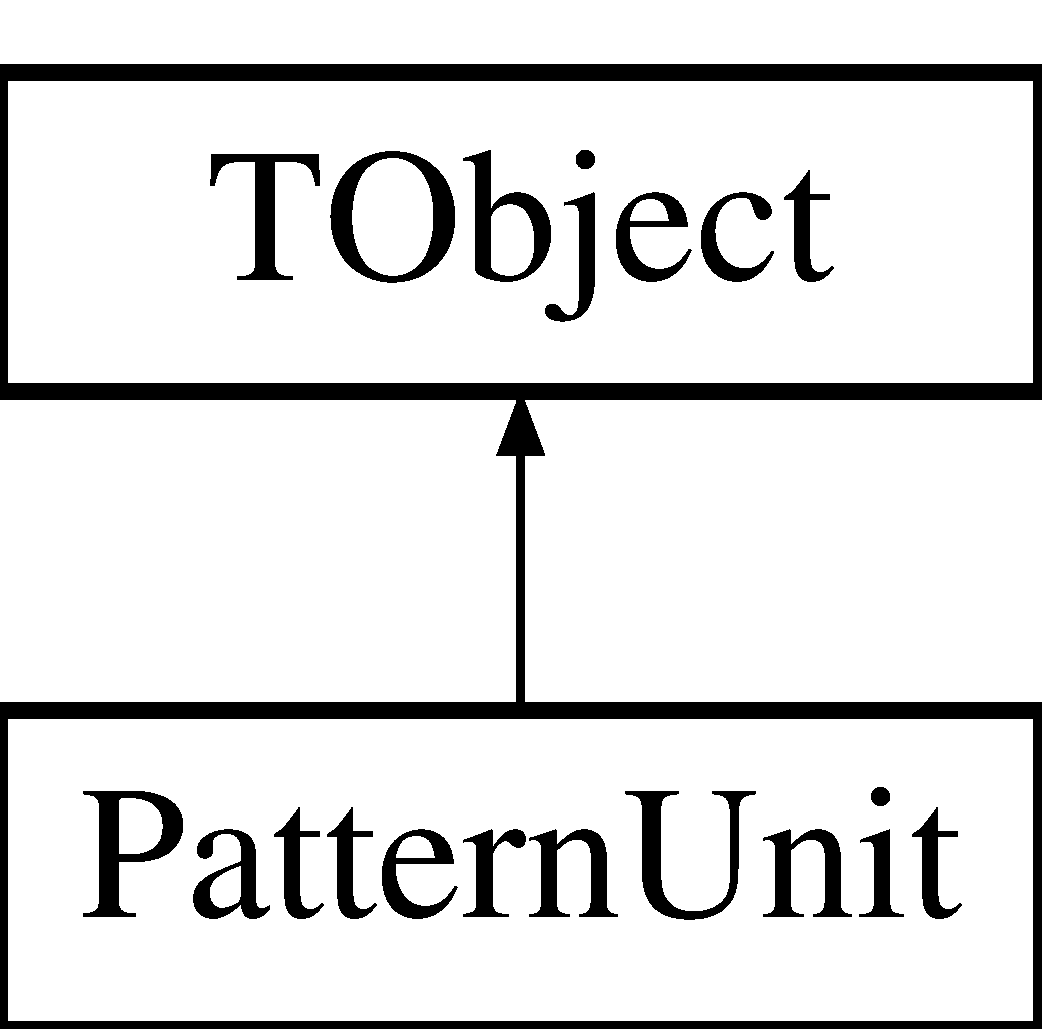
\includegraphics[height=2.000000cm]{class_pattern_unit}
\end{center}
\end{figure}
\subsection*{Public Member Functions}
\begin{DoxyCompactItemize}
\item 
\hypertarget{class_pattern_unit_ac9996fb9db38fad22cd57fce80f6dd77}{void {\bfseries Clear\-Evt} ()}\label{class_pattern_unit_ac9996fb9db38fad22cd57fce80f6dd77}

\item 
\hypertarget{class_pattern_unit_a14ae7bedf1a45782eec52f50d3ae4349}{void {\bfseries Set\-Module\-Number} (unsigned short module\-Number)}\label{class_pattern_unit_a14ae7bedf1a45782eec52f50d3ae4349}

\item 
\hypertarget{class_pattern_unit_a9d34e1e9f1a313afb387a008f10fc1e5}{void {\bfseries Add\-Sub\-Event} (\hyperlink{class_pattern_unit_sub_event}{Pattern\-Unit\-Sub\-Event} Sub\-Event)}\label{class_pattern_unit_a9d34e1e9f1a313afb387a008f10fc1e5}

\item 
\hypertarget{class_pattern_unit_afc5e06336605ed36e329017cf96e7ba9}{size\-\_\-t {\bfseries Get\-Number\-Of\-Sub\-Events} ()}\label{class_pattern_unit_afc5e06336605ed36e329017cf96e7ba9}

\item 
\hypertarget{class_pattern_unit_a76203a82503fc512426839b394bb39d3}{unsigned short {\bfseries Get\-Module\-Number} ()}\label{class_pattern_unit_a76203a82503fc512426839b394bb39d3}

\item 
\hypertarget{class_pattern_unit_ae664a0f15c9b3b6fe3809b68838b9522}{\hyperlink{class_pattern_unit_sub_event}{Pattern\-Unit\-Sub\-Event} $\ast$ {\bfseries Get\-Sub\-Event} (size\-\_\-t Index)}\label{class_pattern_unit_ae664a0f15c9b3b6fe3809b68838b9522}

\item 
\hypertarget{class_pattern_unit_a914db6bc2faec9ee115aa8006be3fbf8}{\hyperlink{class_pattern_unit_sub_event}{Pattern\-Unit\-Sub\-Event} {\bfseries Get\-Last\-Sub\-Event} ()}\label{class_pattern_unit_a914db6bc2faec9ee115aa8006be3fbf8}

\item 
\hypertarget{class_pattern_unit_ab2eba4fd8bb10266198efb2aea53a789}{unsigned short {\bfseries Get\-Number\-Of\-Triggers} ()}\label{class_pattern_unit_ab2eba4fd8bb10266198efb2aea53a789}

\item 
\hypertarget{class_pattern_unit_abac0e1b9460239ec7cbcdb050f995193}{bool {\bfseries Laser\-On} ()}\label{class_pattern_unit_abac0e1b9460239ec7cbcdb050f995193}

\item 
\hypertarget{class_pattern_unit_a2613100013a287640343ed0a791efaff}{bool {\bfseries Field\-Up} ()}\label{class_pattern_unit_a2613100013a287640343ed0a791efaff}

\item 
\hypertarget{class_pattern_unit_abaae7087af48725d48c8231e81ac9c7d}{bool {\bfseries Field\-Down} ()}\label{class_pattern_unit_abaae7087af48725d48c8231e81ac9c7d}

\end{DoxyCompactItemize}
\subsection*{Protected Attributes}
\begin{DoxyCompactItemize}
\item 
\hypertarget{class_pattern_unit_a23d9e67b29f7a16af89cea12293f0d4b}{unsigned short {\bfseries Module\-Number}}\label{class_pattern_unit_a23d9e67b29f7a16af89cea12293f0d4b}

\item 
\hypertarget{class_pattern_unit_ac405794a8bdd20dc9dd249ee0251677c}{vector$<$ \hyperlink{class_pattern_unit_sub_event}{Pattern\-Unit\-Sub\-Event} $>$ {\bfseries Sub\-Events}}\label{class_pattern_unit_ac405794a8bdd20dc9dd249ee0251677c}

\end{DoxyCompactItemize}


The documentation for this class was generated from the following files\-:\begin{DoxyCompactItemize}
\item 
Med\-To\-Root/Modules.\-hh\item 
Med\-To\-Root/Modules.\-cc\end{DoxyCompactItemize}

\hypertarget{class_pattern_unit_sub_event}{}\section{Pattern\+Unit\+Sub\+Event Class Reference}
\label{class_pattern_unit_sub_event}\index{Pattern\+Unit\+Sub\+Event@{Pattern\+Unit\+Sub\+Event}}
Inheritance diagram for Pattern\+Unit\+Sub\+Event\+:\begin{figure}[H]
\begin{center}
\leavevmode
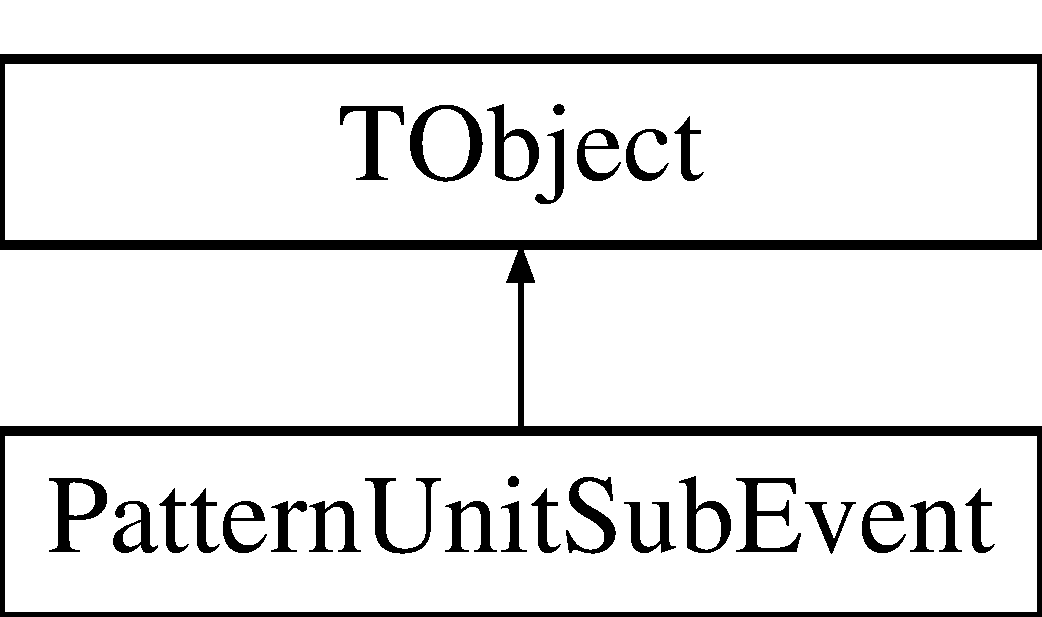
\includegraphics[height=2.000000cm]{class_pattern_unit_sub_event}
\end{center}
\end{figure}
\subsection*{Public Member Functions}
\begin{DoxyCompactItemize}
\item 
\mbox{\Hypertarget{class_pattern_unit_sub_event_aba30013326ba5858d57f134d89ea3669}\label{class_pattern_unit_sub_event_aba30013326ba5858d57f134d89ea3669}} 
size\+\_\+t {\bfseries Size} ()
\item 
\mbox{\Hypertarget{class_pattern_unit_sub_event_ae24f02b44fdad9608018c4df754121f1}\label{class_pattern_unit_sub_event_ae24f02b44fdad9608018c4df754121f1}} 
void {\bfseries Clear\+Evt} ()
\item 
\mbox{\Hypertarget{class_pattern_unit_sub_event_ab9650520294b06b3355072b18908199b}\label{class_pattern_unit_sub_event_ab9650520294b06b3355072b18908199b}} 
void {\bfseries Add} (unsigned int Value)
\item 
\mbox{\Hypertarget{class_pattern_unit_sub_event_a23ec29db91688feaa0de22ca730e8a77}\label{class_pattern_unit_sub_event_a23ec29db91688feaa0de22ca730e8a77}} 
unsigned int {\bfseries Get\+Value} (unsigned short Index)
\item 
\mbox{\Hypertarget{class_pattern_unit_sub_event_a7890f56b171c95b7d90c0f9932bfc879}\label{class_pattern_unit_sub_event_a7890f56b171c95b7d90c0f9932bfc879}} 
unsigned int {\bfseries Get\+Last\+Value} ()
\end{DoxyCompactItemize}
\subsection*{Protected Attributes}
\begin{DoxyCompactItemize}
\item 
\mbox{\Hypertarget{class_pattern_unit_sub_event_ad8b61039fa93af3c377b739a47c917ab}\label{class_pattern_unit_sub_event_ad8b61039fa93af3c377b739a47c917ab}} 
vector$<$ unsigned int $>$ {\bfseries Values}
\end{DoxyCompactItemize}


The documentation for this class was generated from the following files\+:\begin{DoxyCompactItemize}
\item 
Med\+To\+Root/Sub\+Events.\+hh\item 
Med\+To\+Root/Sub\+Events.\+cc\end{DoxyCompactItemize}

\hypertarget{class_scaler_sub_event}{}\section{Scaler\+Sub\+Event Class Reference}
\label{class_scaler_sub_event}\index{Scaler\+Sub\+Event@{Scaler\+Sub\+Event}}
Inheritance diagram for Scaler\+Sub\+Event\+:\begin{figure}[H]
\begin{center}
\leavevmode
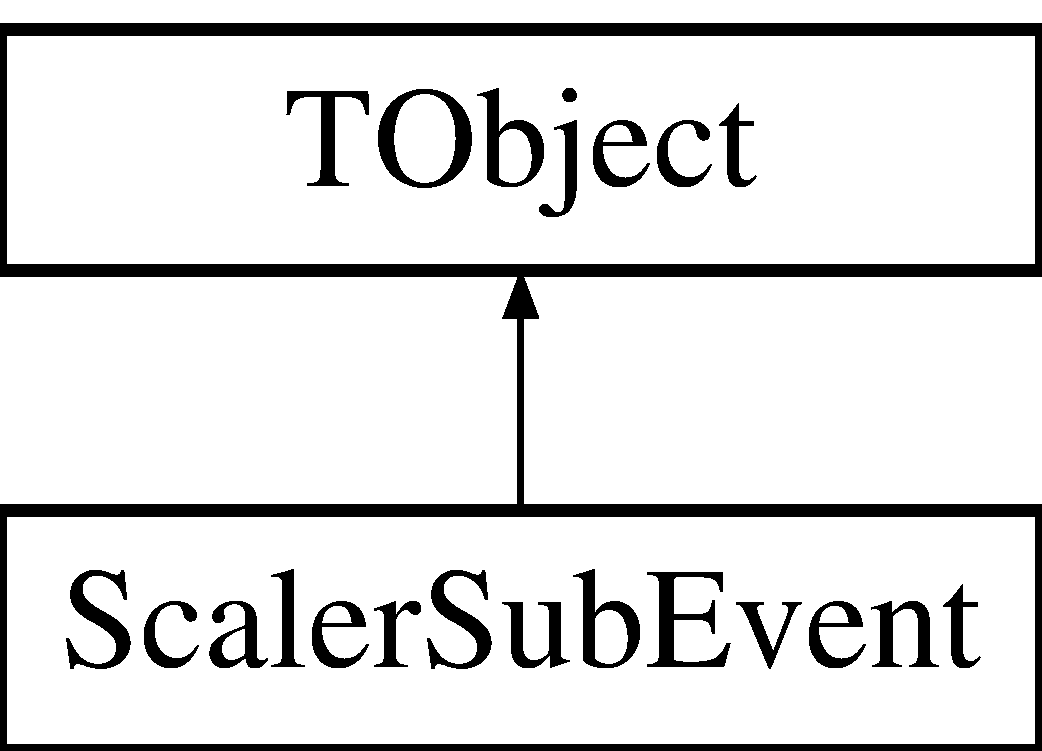
\includegraphics[height=2.000000cm]{class_scaler_sub_event}
\end{center}
\end{figure}
\subsection*{Public Member Functions}
\begin{DoxyCompactItemize}
\item 
\mbox{\Hypertarget{class_scaler_sub_event_a5db34a3f53c89bad6d9a961132cad259}\label{class_scaler_sub_event_a5db34a3f53c89bad6d9a961132cad259}} 
size\+\_\+t {\bfseries Size} ()
\item 
\mbox{\Hypertarget{class_scaler_sub_event_abd5effab974e0d49409556603e614c5a}\label{class_scaler_sub_event_abd5effab974e0d49409556603e614c5a}} 
void {\bfseries Clear\+Evt} ()
\item 
\mbox{\Hypertarget{class_scaler_sub_event_a4958f75ee49941fece531ac3924fe2e3}\label{class_scaler_sub_event_a4958f75ee49941fece531ac3924fe2e3}} 
void {\bfseries Add} (unsigned short Channel, unsigned int Value)
\item 
\mbox{\Hypertarget{class_scaler_sub_event_ab728020f4bffbf31be733bd14be29884}\label{class_scaler_sub_event_ab728020f4bffbf31be733bd14be29884}} 
unsigned short {\bfseries Get\+Channel} (unsigned short Index)
\item 
\mbox{\Hypertarget{class_scaler_sub_event_ac47b65fbb194003c8183db5a1a277f5d}\label{class_scaler_sub_event_ac47b65fbb194003c8183db5a1a277f5d}} 
unsigned int {\bfseries Get\+Value} (unsigned short Index)
\item 
\mbox{\Hypertarget{class_scaler_sub_event_a3731af3cd6dbb0063051fb9a309d9c44}\label{class_scaler_sub_event_a3731af3cd6dbb0063051fb9a309d9c44}} 
unsigned short {\bfseries Get\+Last\+Channel} ()
\item 
\mbox{\Hypertarget{class_scaler_sub_event_a9cebf7678667cbd4a8976b4544df7a1d}\label{class_scaler_sub_event_a9cebf7678667cbd4a8976b4544df7a1d}} 
unsigned int {\bfseries Get\+Last\+Value} ()
\end{DoxyCompactItemize}
\subsection*{Protected Attributes}
\begin{DoxyCompactItemize}
\item 
\mbox{\Hypertarget{class_scaler_sub_event_aaedde4ea0a9fb4c43afaada4863d3173}\label{class_scaler_sub_event_aaedde4ea0a9fb4c43afaada4863d3173}} 
vector$<$ unsigned short $>$ {\bfseries Channels}
\item 
\mbox{\Hypertarget{class_scaler_sub_event_ac07cb50429e195455d77552394c2c486}\label{class_scaler_sub_event_ac07cb50429e195455d77552394c2c486}} 
vector$<$ unsigned int $>$ {\bfseries Values}
\end{DoxyCompactItemize}


The documentation for this class was generated from the following files\+:\begin{DoxyCompactItemize}
\item 
Med\+To\+Root/Sub\+Events.\+hh\item 
Med\+To\+Root/Sub\+Events.\+cc\end{DoxyCompactItemize}

\hypertarget{class_s_i_s_scaler}{}\section{S\+I\+S\+Scaler Class Reference}
\label{class_s_i_s_scaler}\index{S\+I\+S\+Scaler@{S\+I\+S\+Scaler}}
Inheritance diagram for S\+I\+S\+Scaler\+:\begin{figure}[H]
\begin{center}
\leavevmode
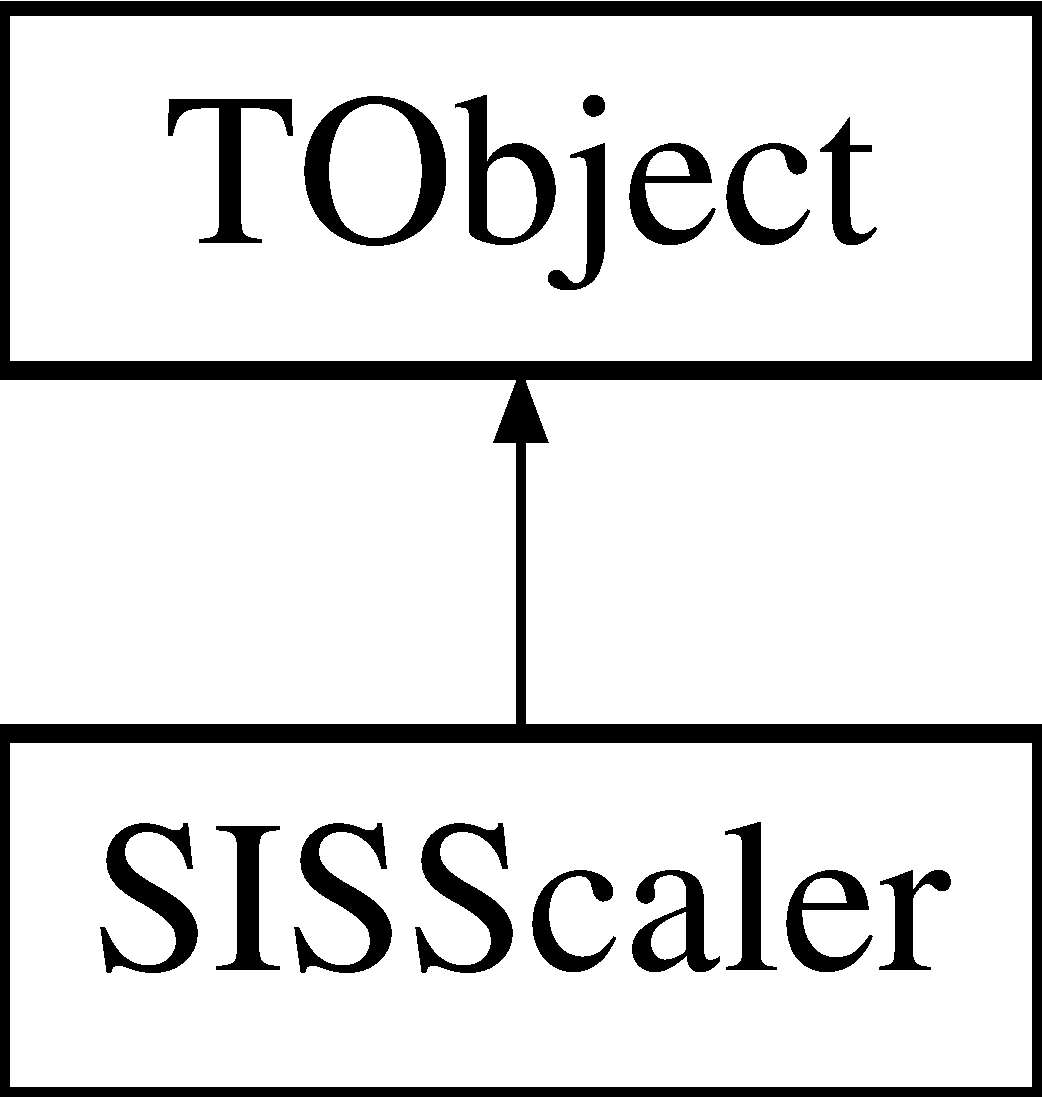
\includegraphics[height=2.000000cm]{class_s_i_s_scaler}
\end{center}
\end{figure}
\subsection*{Public Member Functions}
\begin{DoxyCompactItemize}
\item 
\mbox{\Hypertarget{class_s_i_s_scaler_a1038e9479e85008d7283bb10d3a0ea52}\label{class_s_i_s_scaler_a1038e9479e85008d7283bb10d3a0ea52}} 
void {\bfseries Clear\+Evt} ()
\item 
\mbox{\Hypertarget{class_s_i_s_scaler_a19a3c1b9b24d6dd3f359c25749cca97b}\label{class_s_i_s_scaler_a19a3c1b9b24d6dd3f359c25749cca97b}} 
void {\bfseries Set\+Module\+Number} (unsigned short module\+Number)
\item 
\mbox{\Hypertarget{class_s_i_s_scaler_acd7452d99f825be03e150ca7095e81f2}\label{class_s_i_s_scaler_acd7452d99f825be03e150ca7095e81f2}} 
void {\bfseries Add\+Sub\+Event} (\hyperlink{class_scaler_sub_event}{Scaler\+Sub\+Event} Sub\+Event)
\item 
\mbox{\Hypertarget{class_s_i_s_scaler_aa0fc0b485191e72ef46ed4fccb9525e1}\label{class_s_i_s_scaler_aa0fc0b485191e72ef46ed4fccb9525e1}} 
size\+\_\+t {\bfseries Get\+Number\+Of\+Sub\+Events} ()
\item 
\mbox{\Hypertarget{class_s_i_s_scaler_aa3c573faebe1e226c94834515f94cfe4}\label{class_s_i_s_scaler_aa3c573faebe1e226c94834515f94cfe4}} 
unsigned short {\bfseries Get\+Module\+Number} ()
\item 
\mbox{\Hypertarget{class_s_i_s_scaler_a8596170dd427752af3c9e2343971e07c}\label{class_s_i_s_scaler_a8596170dd427752af3c9e2343971e07c}} 
\hyperlink{class_scaler_sub_event}{Scaler\+Sub\+Event} $\ast$ {\bfseries Get\+Sub\+Event} (size\+\_\+t Index)
\item 
\mbox{\Hypertarget{class_s_i_s_scaler_a2fc33da7a9676cc15912ead53f72ff06}\label{class_s_i_s_scaler_a2fc33da7a9676cc15912ead53f72ff06}} 
\hyperlink{class_scaler_sub_event}{Scaler\+Sub\+Event} {\bfseries Get\+Last\+Sub\+Event} ()
\end{DoxyCompactItemize}
\subsection*{Protected Attributes}
\begin{DoxyCompactItemize}
\item 
\mbox{\Hypertarget{class_s_i_s_scaler_a4265cde97345c344d921d5eb1be0df50}\label{class_s_i_s_scaler_a4265cde97345c344d921d5eb1be0df50}} 
unsigned short {\bfseries Module\+Number}
\item 
\mbox{\Hypertarget{class_s_i_s_scaler_a671eb8d858f9d2d4550fe76a89cf3095}\label{class_s_i_s_scaler_a671eb8d858f9d2d4550fe76a89cf3095}} 
vector$<$ \hyperlink{class_scaler_sub_event}{Scaler\+Sub\+Event} $>$ {\bfseries Sub\+Events}
\end{DoxyCompactItemize}


The documentation for this class was generated from the following files\+:\begin{DoxyCompactItemize}
\item 
Med\+To\+Root/Modules.\+hh\item 
Med\+To\+Root/Modules.\+cc\end{DoxyCompactItemize}

\hypertarget{class_spede_geometry}{}\section{Spede\+Geometry Class Reference}
\label{class_spede_geometry}\index{Spede\+Geometry@{Spede\+Geometry}}
\subsection*{Public Member Functions}
\begin{DoxyCompactItemize}
\item 
\mbox{\Hypertarget{class_spede_geometry_aff2cf68512c9a78eb117ff1ea44e95f0}\label{class_spede_geometry_aff2cf68512c9a78eb117ff1ea44e95f0}} 
void {\bfseries Setup\+Spede} ()
\item 
\mbox{\Hypertarget{class_spede_geometry_ae79185d5c0e1d21a1a26ef824038ce9c}\label{class_spede_geometry_ae79185d5c0e1d21a1a26ef824038ce9c}} 
void {\bfseries Setup\+Spede} (double user\+\_\+r, double user\+\_\+alpha)
\item 
\mbox{\Hypertarget{class_spede_geometry_ad17f4485ee83860a40082d8c8af5237c}\label{class_spede_geometry_ad17f4485ee83860a40082d8c8af5237c}} 
void {\bfseries Set\+SpedeR} (double user\+\_\+r)
\item 
\mbox{\Hypertarget{class_spede_geometry_a94c3f5b2dbf4490db7d72514c8abe340}\label{class_spede_geometry_a94c3f5b2dbf4490db7d72514c8abe340}} 
void {\bfseries Set\+Spede\+Alpha} (double user\+\_\+alpha)
\item 
\mbox{\Hypertarget{class_spede_geometry_a05865b0752fb518337a9a16f8fba9085}\label{class_spede_geometry_a05865b0752fb518337a9a16f8fba9085}} 
double {\bfseries Get\+Spede\+Theta} (int seg)
\item 
\mbox{\Hypertarget{class_spede_geometry_a93bd92636bce1259b189bb17275d238d}\label{class_spede_geometry_a93bd92636bce1259b189bb17275d238d}} 
double {\bfseries Get\+Spede\+Phi} (int seg)
\item 
\mbox{\Hypertarget{class_spede_geometry_aff2cf68512c9a78eb117ff1ea44e95f0}\label{class_spede_geometry_aff2cf68512c9a78eb117ff1ea44e95f0}} 
void {\bfseries Setup\+Spede} ()
\item 
\mbox{\Hypertarget{class_spede_geometry_ae79185d5c0e1d21a1a26ef824038ce9c}\label{class_spede_geometry_ae79185d5c0e1d21a1a26ef824038ce9c}} 
void {\bfseries Setup\+Spede} (double user\+\_\+r, double user\+\_\+alpha)
\item 
\mbox{\Hypertarget{class_spede_geometry_ad17f4485ee83860a40082d8c8af5237c}\label{class_spede_geometry_ad17f4485ee83860a40082d8c8af5237c}} 
void {\bfseries Set\+SpedeR} (double user\+\_\+r)
\item 
\mbox{\Hypertarget{class_spede_geometry_a94c3f5b2dbf4490db7d72514c8abe340}\label{class_spede_geometry_a94c3f5b2dbf4490db7d72514c8abe340}} 
void {\bfseries Set\+Spede\+Alpha} (double user\+\_\+alpha)
\item 
\mbox{\Hypertarget{class_spede_geometry_a05865b0752fb518337a9a16f8fba9085}\label{class_spede_geometry_a05865b0752fb518337a9a16f8fba9085}} 
double {\bfseries Get\+Spede\+Theta} (int seg)
\item 
\mbox{\Hypertarget{class_spede_geometry_a93bd92636bce1259b189bb17275d238d}\label{class_spede_geometry_a93bd92636bce1259b189bb17275d238d}} 
double {\bfseries Get\+Spede\+Phi} (int seg)
\item 
\mbox{\Hypertarget{class_spede_geometry_aff2cf68512c9a78eb117ff1ea44e95f0}\label{class_spede_geometry_aff2cf68512c9a78eb117ff1ea44e95f0}} 
void {\bfseries Setup\+Spede} ()
\item 
\mbox{\Hypertarget{class_spede_geometry_ae79185d5c0e1d21a1a26ef824038ce9c}\label{class_spede_geometry_ae79185d5c0e1d21a1a26ef824038ce9c}} 
void {\bfseries Setup\+Spede} (double user\+\_\+r, double user\+\_\+alpha)
\item 
\mbox{\Hypertarget{class_spede_geometry_ad17f4485ee83860a40082d8c8af5237c}\label{class_spede_geometry_ad17f4485ee83860a40082d8c8af5237c}} 
void {\bfseries Set\+SpedeR} (double user\+\_\+r)
\item 
\mbox{\Hypertarget{class_spede_geometry_a94c3f5b2dbf4490db7d72514c8abe340}\label{class_spede_geometry_a94c3f5b2dbf4490db7d72514c8abe340}} 
void {\bfseries Set\+Spede\+Alpha} (double user\+\_\+alpha)
\item 
\mbox{\Hypertarget{class_spede_geometry_a05865b0752fb518337a9a16f8fba9085}\label{class_spede_geometry_a05865b0752fb518337a9a16f8fba9085}} 
double {\bfseries Get\+Spede\+Theta} (int seg)
\item 
\mbox{\Hypertarget{class_spede_geometry_a93bd92636bce1259b189bb17275d238d}\label{class_spede_geometry_a93bd92636bce1259b189bb17275d238d}} 
double {\bfseries Get\+Spede\+Phi} (int seg)
\end{DoxyCompactItemize}


The documentation for this class was generated from the following files\+:\begin{DoxyCompactItemize}
\item 
C\+L\+X\+Ana/Spede\+Geometry.\+hh\item 
C\+L\+X\+Ana/Spede\+Geometry.\+cc\end{DoxyCompactItemize}

\hypertarget{class_unpacked_event}{\section{Unpacked\-Event Class Reference}
\label{class_unpacked_event}\index{Unpacked\-Event@{Unpacked\-Event}}
}
Inheritance diagram for Unpacked\-Event\-:\begin{figure}[H]
\begin{center}
\leavevmode
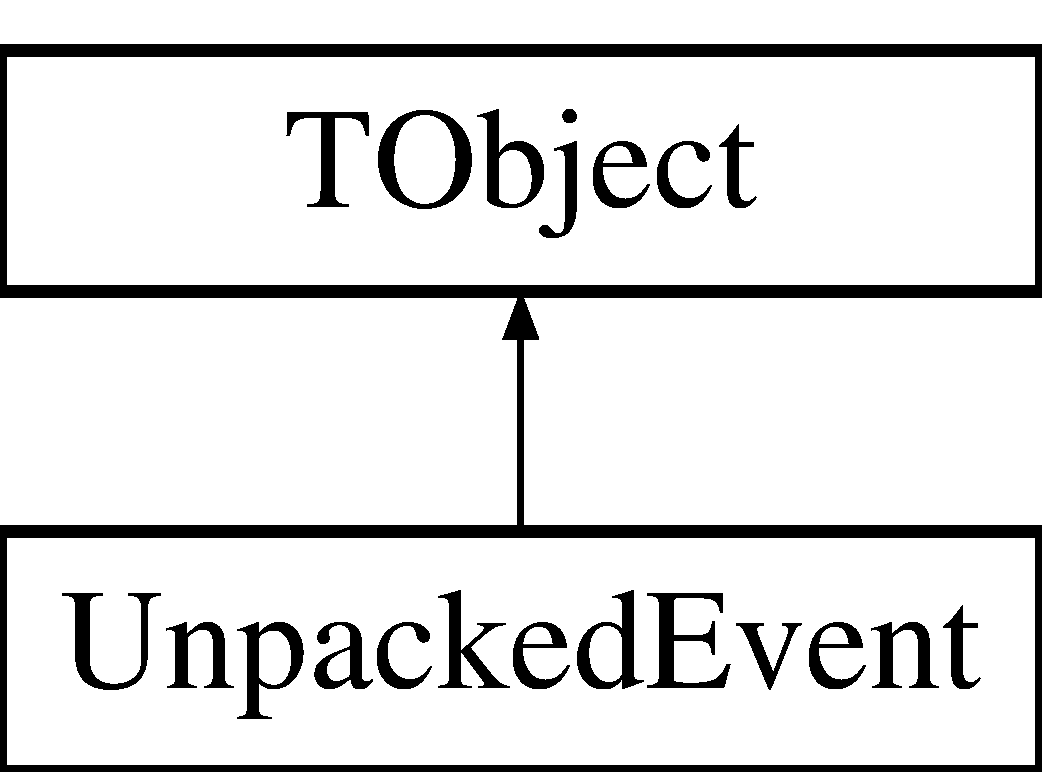
\includegraphics[height=2.000000cm]{class_unpacked_event}
\end{center}
\end{figure}
\subsection*{Public Member Functions}
\begin{DoxyCompactItemize}
\item 
\hypertarget{class_unpacked_event_a399f80fef86fdaf260c67d0868e39006}{{\bfseries Unpacked\-Event} (\hyperlink{class_global_settings}{Global\-Settings} $\ast$)}\label{class_unpacked_event_a399f80fef86fdaf260c67d0868e39006}

\item 
\hypertarget{class_unpacked_event_a719e676645566cd033f53ad047fea2e8}{int {\bfseries Process\-Event} (const M\-B\-S\-Data\-I\-O $\ast$)}\label{class_unpacked_event_a719e676645566cd033f53ad047fea2e8}

\item 
\hypertarget{class_unpacked_event_a654a1c6f241b56cf4e3cb18606e98101}{bool {\bfseries Extract\-Subevents} (const M\-B\-S\-Data\-I\-O $\ast$)}\label{class_unpacked_event_a654a1c6f241b56cf4e3cb18606e98101}

\item 
\hypertarget{class_unpacked_event_a1473955edd8aced26b25f4aa4ea1cc99}{bool {\bfseries Decode\-Dgf} (int, int, char $\ast$)}\label{class_unpacked_event_a1473955edd8aced26b25f4aa4ea1cc99}

\item 
\hypertarget{class_unpacked_event_a5d1e95803242426e747e325bf5f41882}{bool {\bfseries Decode\-Adc} (int, int, char $\ast$)}\label{class_unpacked_event_a5d1e95803242426e747e325bf5f41882}

\item 
\hypertarget{class_unpacked_event_a8622b91904185be6dbca1b27d629d3b3}{bool {\bfseries Decode\-Mesytec\-Adc} (int, int, char $\ast$)}\label{class_unpacked_event_a8622b91904185be6dbca1b27d629d3b3}

\item 
\hypertarget{class_unpacked_event_aace1ccd22e30b9b188b06db28e406ef2}{bool {\bfseries Decode\-S\-I\-S3600\-Pattern\-Unit} (int, int, char $\ast$)}\label{class_unpacked_event_aace1ccd22e30b9b188b06db28e406ef2}

\item 
\hypertarget{class_unpacked_event_adbce67a2bb15ce234e133ce686324762}{bool {\bfseries Decode\-Bragg\-Chamber} (int, int, char $\ast$)}\label{class_unpacked_event_adbce67a2bb15ce234e133ce686324762}

\item 
\hypertarget{class_unpacked_event_a9b1491e6809f949d582348f4855671a9}{bool {\bfseries Decode\-Scaler} (int, int, char $\ast$)}\label{class_unpacked_event_a9b1491e6809f949d582348f4855671a9}

\item 
\hypertarget{class_unpacked_event_a7a965ea80344bfb2957dc68495085bd4}{bool {\bfseries Decode\-Dgf\-Scaler} (int, int, char $\ast$)}\label{class_unpacked_event_a7a965ea80344bfb2957dc68495085bd4}

\item 
\hypertarget{class_unpacked_event_a8a2410a51de9fdfa467866b4d041cd51}{void {\bfseries Set\-Dgf\-Module} (size\-\_\-t Index, \hyperlink{class_dgf_module}{Dgf\-Module} New\-Dgf\-Module)}\label{class_unpacked_event_a8a2410a51de9fdfa467866b4d041cd51}

\item 
\hypertarget{class_unpacked_event_ad0cf4ae46cfc609594ca67b55a98c2fc}{void {\bfseries Set\-Adc\-Module} (size\-\_\-t Index, \hyperlink{class_adc_module}{Adc\-Module} New\-Adc\-Module)}\label{class_unpacked_event_ad0cf4ae46cfc609594ca67b55a98c2fc}

\item 
\hypertarget{class_unpacked_event_a44f6c5ae5cc6e6103be86a776730b603}{void {\bfseries Set\-Pattern\-Unit} (size\-\_\-t Index, \hyperlink{class_pattern_unit}{Pattern\-Unit} New\-Pattern\-Unit)}\label{class_unpacked_event_a44f6c5ae5cc6e6103be86a776730b603}

\item 
\hypertarget{class_unpacked_event_a664861c77ddac5439a82b376982a82d4}{void {\bfseries Clear\-Evt} ()}\label{class_unpacked_event_a664861c77ddac5439a82b376982a82d4}

\item 
\hypertarget{class_unpacked_event_a99fe4883b6afaeeb7323942dc4c2df35}{bool {\bfseries Verify} ()}\label{class_unpacked_event_a99fe4883b6afaeeb7323942dc4c2df35}

\item 
\hypertarget{class_unpacked_event_ad041cb52b49e07a5abd74956f25d8d6e}{long long {\bfseries Get\-Event\-Number} ()}\label{class_unpacked_event_ad041cb52b49e07a5abd74956f25d8d6e}

\item 
\hypertarget{class_unpacked_event_a8411c29339ab3d12ead8dc040f5eb124}{int {\bfseries Get\-Number\-Of\-Dgf\-Modules} ()}\label{class_unpacked_event_a8411c29339ab3d12ead8dc040f5eb124}

\item 
\hypertarget{class_unpacked_event_a17961a5669eeee7f7d8e864d7d59e031}{int {\bfseries Get\-Number\-Of\-Adc\-Modules} ()}\label{class_unpacked_event_a17961a5669eeee7f7d8e864d7d59e031}

\item 
\hypertarget{class_unpacked_event_a6513a1facbdd44bc401e3ddb1d4c7e0e}{int {\bfseries Get\-Number\-Of\-Pattern\-Units} ()}\label{class_unpacked_event_a6513a1facbdd44bc401e3ddb1d4c7e0e}

\item 
\hypertarget{class_unpacked_event_a3dc0fa2fb893c935047e3fe28e7a0ab3}{\hyperlink{class_dgf_module}{Dgf\-Module} $\ast$ {\bfseries Get\-Dgf\-Module} (size\-\_\-t Index)}\label{class_unpacked_event_a3dc0fa2fb893c935047e3fe28e7a0ab3}

\item 
\hypertarget{class_unpacked_event_a481fd2e7637bb38890e2e12ae51b4bcc}{\hyperlink{class_adc_module}{Adc\-Module} $\ast$ {\bfseries Get\-Adc\-Module} (size\-\_\-t Index)}\label{class_unpacked_event_a481fd2e7637bb38890e2e12ae51b4bcc}

\item 
\hypertarget{class_unpacked_event_a745192df038ac608501642b12e362460}{\hyperlink{class_pattern_unit}{Pattern\-Unit} $\ast$ {\bfseries Get\-Pattern\-Unit} (size\-\_\-t Index)}\label{class_unpacked_event_a745192df038ac608501642b12e362460}

\item 
\hypertarget{class_unpacked_event_afea632b950f2cf8ea9fa04b1f5524c38}{\hyperlink{class_dgf_module}{Dgf\-Module} $\ast$ {\bfseries Get\-Timestamp\-Module} (size\-\_\-t Index)}\label{class_unpacked_event_afea632b950f2cf8ea9fa04b1f5524c38}

\item 
\hypertarget{class_unpacked_event_a7ac2922807426765fc158f7171e6ae06}{unsigned short {\bfseries Get\-Timestamps} (vector$<$ unsigned short $>$ \&)}\label{class_unpacked_event_a7ac2922807426765fc158f7171e6ae06}

\item 
\hypertarget{class_unpacked_event_a1823ddca4adcbc26861072ff45bcc737}{unsigned short {\bfseries Get\-Timestamps} (unsigned short)}\label{class_unpacked_event_a1823ddca4adcbc26861072ff45bcc737}

\item 
\hypertarget{class_unpacked_event_aecb283a228b877c6644ab0da5ba1aa96}{\hyperlink{class_dgf_module}{Dgf\-Module} $\ast$ {\bfseries Get\-Ebis\-T1\-And\-Super\-Cycle\-Module} ()}\label{class_unpacked_event_aecb283a228b877c6644ab0da5ba1aa96}

\item 
\hypertarget{class_unpacked_event_a9a7536c85e4cdbf09e8cd9e8960c67a6}{bool {\bfseries Scaler\-Data} ()}\label{class_unpacked_event_a9a7536c85e4cdbf09e8cd9e8960c67a6}

\item 
\hypertarget{class_unpacked_event_a779dc661d6fe806b5cac503984943439}{\hyperlink{class_s_i_s_scaler}{S\-I\-S\-Scaler} $\ast$ {\bfseries Get\-Scaler} ()}\label{class_unpacked_event_a779dc661d6fe806b5cac503984943439}

\item 
\hypertarget{class_unpacked_event_af4a9a5fcfd0b2658e167f64c67c73068}{\hyperlink{class_dgf_scaler}{Dgf\-Scaler} $\ast$ {\bfseries Get\-Dgf\-Scaler} ()}\label{class_unpacked_event_af4a9a5fcfd0b2658e167f64c67c73068}

\item 
\hypertarget{class_unpacked_event_aaeac1edfe26995fb9c8f4b7349f0cc79}{\hyperlink{class_bragg_chamber}{Bragg\-Chamber} $\ast$ {\bfseries Get\-Bragg\-Chamber} ()}\label{class_unpacked_event_aaeac1edfe26995fb9c8f4b7349f0cc79}

\item 
\hypertarget{class_unpacked_event_a9860faeecdcbc7758d0889c9bd8f51de}{void {\bfseries Statistics} ()}\label{class_unpacked_event_a9860faeecdcbc7758d0889c9bd8f51de}

\end{DoxyCompactItemize}
\subsection*{Protected Attributes}
\begin{DoxyCompactItemize}
\item 
\hypertarget{class_unpacked_event_af05cdc5cd976188aa4d876d48265dd4e}{\hyperlink{class_global_settings}{Global\-Settings} $\ast$ {\bfseries Settings}}\label{class_unpacked_event_af05cdc5cd976188aa4d876d48265dd4e}

\item 
\hypertarget{class_unpacked_event_ad798c6e08da59b6964c5ad2b3bee4cde}{unsigned long long {\bfseries Event\-Number}}\label{class_unpacked_event_ad798c6e08da59b6964c5ad2b3bee4cde}

\item 
\hypertarget{class_unpacked_event_a3930bce3510be78df4058f5107a15313}{unsigned long long {\bfseries Wrong\-Hit\-Pattern}}\label{class_unpacked_event_a3930bce3510be78df4058f5107a15313}

\item 
\hypertarget{class_unpacked_event_a1011d28310c7f0f5dbbb8414ddb616a8}{unsigned long long {\bfseries Wrong\-Adc\-Header}}\label{class_unpacked_event_a1011d28310c7f0f5dbbb8414ddb616a8}

\item 
\hypertarget{class_unpacked_event_aeef1201a91a0280b7c88e4b8ddf7a2d3}{unsigned long long {\bfseries Adc\-Overflow}}\label{class_unpacked_event_aeef1201a91a0280b7c88e4b8ddf7a2d3}

\item 
\hypertarget{class_unpacked_event_a19ba633f09a9d52648d095118536b3b2}{unsigned long long {\bfseries Adc\-Underflow}}\label{class_unpacked_event_a19ba633f09a9d52648d095118536b3b2}

\item 
\hypertarget{class_unpacked_event_af4bb3effdfadd4a684a4296931be1379}{vector$<$ \hyperlink{class_dgf_module}{Dgf\-Module} $>$ {\bfseries Dgf\-Modules}}\label{class_unpacked_event_af4bb3effdfadd4a684a4296931be1379}

\item 
\hypertarget{class_unpacked_event_a023f5c7816352ca7b49cc8908ce37546}{vector$<$ \hyperlink{class_adc_module}{Adc\-Module} $>$ {\bfseries Adc\-Modules}}\label{class_unpacked_event_a023f5c7816352ca7b49cc8908ce37546}

\item 
\hypertarget{class_unpacked_event_a147d614bb78b22864dc99425bdc955cc}{vector$<$ \hyperlink{class_pattern_unit}{Pattern\-Unit} $>$ {\bfseries Pattern\-Units}}\label{class_unpacked_event_a147d614bb78b22864dc99425bdc955cc}

\item 
\hypertarget{class_unpacked_event_a88d4f6879caf81bed72049adb9f88802}{\hyperlink{class_s_i_s_scaler}{S\-I\-S\-Scaler} {\bfseries Scaler}}\label{class_unpacked_event_a88d4f6879caf81bed72049adb9f88802}

\item 
\hypertarget{class_unpacked_event_ad0a12f7dec89cf5cad8f7df4c2fe5013}{\hyperlink{class_dgf_scaler}{Dgf\-Scaler} {\bfseries f\-Dgf\-Scaler}}\label{class_unpacked_event_ad0a12f7dec89cf5cad8f7df4c2fe5013}

\item 
\hypertarget{class_unpacked_event_ac705f3a8de8500aeb6f7cb3951b76d0e}{\hyperlink{class_bragg_chamber}{Bragg\-Chamber} {\bfseries f\-Bragg\-Chamber}}\label{class_unpacked_event_ac705f3a8de8500aeb6f7cb3951b76d0e}

\item 
\hypertarget{class_unpacked_event_a13011a375b40157797fbd84e4a4fd092}{bool {\bfseries f\-Scaler\-Data}}\label{class_unpacked_event_a13011a375b40157797fbd84e4a4fd092}

\item 
\hypertarget{class_unpacked_event_a46e5d49e6b7fb87cf00e4feb03c2b875}{unsigned int {\bfseries f\-Buffer\-Time}}\label{class_unpacked_event_a46e5d49e6b7fb87cf00e4feb03c2b875}

\end{DoxyCompactItemize}
\subsection*{Private Member Functions}
\begin{DoxyCompactItemize}
\item 
\hypertarget{class_unpacked_event_af6a5c2addbb7e825c9c850e2d7a06c06}{void {\bfseries Correct\-Mesytec\-Adc\-Timestamps} ()}\label{class_unpacked_event_af6a5c2addbb7e825c9c850e2d7a06c06}

\end{DoxyCompactItemize}


The documentation for this class was generated from the following files\-:\begin{DoxyCompactItemize}
\item 
Med\-To\-Root/Unpacked\-Event.\-hh\item 
Med\-To\-Root/Unpacked\-Event.\-cc\end{DoxyCompactItemize}

%--- End generated contents ---

% Index
\backmatter
\newpage
\phantomsection
\clearemptydoublepage
\addcontentsline{toc}{chapter}{Index}
\printindex

\end{document}
